\documentclass[%
paper=a4,       % Papiergröße
fontsize=11pt,  % Schriftgröße
ngerman         % Option für deutsche Sprache
]{scrreprt}
\usepackage{scrhack}
\usepackage{comment} %makes commenting out easier
%Basics für Codierung und Sprache
% ===========================================================
\usepackage{framed}
\usepackage{lipsum}
\usepackage[final]{graphicx}          % Einbindung von Grafiken
\usepackage{placeins}
\usepackage{float}                    % für [H]-Option bei Bildern
\graphicspath{{figs/} {images/}}
\usepackage{subcaption}
\usepackage{babel}                    % deutsche Silbentrennung, etc.
\usepackage[german=quotes]{csquotes}  % deutsche Anführungszeichen mit \enquote{...}
\usepackage{titling}
\usepackage{booktabs} % für tabellen
\RequirePackage[backend=biber, style=numeric, sorting=none, labelalpha=true]{biblatex}     % erlaubt das Einfügen eines Quellenverzeichnisses
% ===========================================================

% Fonts und Typographie
% ===========================================================
%\usepackage{sourcecodepro}
\usepackage[T1]{fontenc}
%\usepackage{lmodern}
%\usepackage{mathptmx}
%\usepackage{mathpazo} % Palatino
%\usepackage{helvet} % Helvetica
%\usepackage{courier} % Courier
%\usepackage{times}
%\usepackage{fix-cm}
%\usepackage{anyfontsize}
%\usepackage[default]{sourcesanspro}
%\usepackage{nimbusmononarrow}

%\usepackage[babel=true,final,tracking=smallcaps]{microtype}
%\DisableLigatures{encoding = T1, family = tt* }   % keine Ligaturen für Monospace-Fonts
% ===========================================================
% Farben
% ===========================================================
\usepackage[x11names]{xcolor}
% ===========================================================

% Mathe-Pakete und -Einstellungen
% ===========================================================
%\usepackage{yhmath}
\usepackage{amsmath}
\usepackage{amsthm}
\usepackage{mathtools}             % Tools zum Setzen von Formeln
\usepackage{amssymb,}               % übliche Mathe-Symbole
\usepackage[bigdelims]{newtxmath}  % moderne Mathe-Font
\allowdisplaybreaks{}               % seitenübergreifende Rechnungen
\usepackage{bm}                    % math bold font
%\usepackage{wasysym}               % noch mehr Symbole
\usepackage{siunitx}
\sisetup{output-decimal-marker = {,}, separate-uncertainty = true} % Kommas als Dezimalteiler
\DeclareSIUnit\barn{b}
\DeclareSIUnit\nm{\nano\metre}
\DeclareSIUnit\mm{\milli\metre}
\DeclareSIUnit\um{\micro\metre}
\DeclareSIUnit\cm{\centi\metre}
\DeclareSIUnit\m{\metre}
\DeclareSIUnit\km{\kilo\metre}
% ===========================================================

% TikZ
% ===========================================================
\usepackage{tikz}
\usetikzlibrary{arrows,arrows.meta}   % mehr Pfeile!
\usetikzlibrary{calc}                 % TikZ kann rechnen
\usetikzlibrary{positioning}
\tikzset{>=Latex}                     % Standard-Pfeilspitze
% ===========================================================

% Seitenlayout, Kopf-/Fußzeile
% ===========================================================
\usepackage[top=3cm, bottom=3cm, left=2.5cm, right=2cm]{geometry}
\RequirePackage[headsepline]{scrlayer-scrpage} % edit header and footer of a page, for more lines add [headtopline, headsepline, footsepline, footbotline]
\pagestyle{scrheadings} % set formatting to scrheadings
\clearpairofpagestyles{}
\setkomafont{pageheadfoot}{}

% ===========================================================

% Hyperref für Referenzen und Hyperlinks
% ===========================================================
\usepackage[%
hidelinks,
pdfpagelabels,
bookmarksopen=true,
bookmarksnumbered=true,
linkcolor=black,
urlcolor=SkyBlue2,
plainpages=false,
pagebackref,
citecolor=black,
hypertexnames=true,
pdfborderstyle={/S/U},
linkbordercolor=SkyBlue2,
colorlinks=false,
backref=false]{hyperref}
\hypersetup{final}
\usepackage{cleveref}
\crefname{figure}{Abb.}{Abb.}
\crefname{table}{Tab.}{Tab.}
\crefname{equation}{Gl.}{Gl.}
% ===========================================================

% Listen und Tabellen
% ===========================================================
\usepackage{multicol}
\usepackage[shortlabels]{enumitem}
\setlist{itemsep=0pt}
\setlist[enumerate]{font=\sffamily\bfseries}
\setlist[itemize]{label=$\triangleright$}
\usepackage{tabularx}
% ===========================================================

% listings
% ===========================================================
\usepackage{listingsutf8}
\lstset{
	belowcaptionskip=1\baselineskip,
	breaklines=true,
	showstringspaces=false,
	basicstyle=\ttfamily,
	keywordstyle=\bfseries\color{green!40!black},
	commentstyle=\itshape\color{purple!40!black},
	stringstyle=\color{orange},
	numbers=left,
	numberstyle=\footnotesize\ttfamily\color{gray},
	inputencoding=utf8/latin1,
	tabsize=4,
}

%%%%%%%%%%%%%%%%%%%%%%%%%%%%%%%%%%%%%%%%%%%%%%%%%%%%%%%%%%%
%%% Ab hier folgen nur noch vordefinierte Shortcuts %%%
%%%%%%%%%%%%%%%%%%%%%%%%%%%%%%%%%%%%%%%%%%%%%%%%%%%%%%%%%%%

\newcommand{\BB}{\mathbb{B}}
\newcommand{\CC}{\mathbb{C}}
\newcommand{\NN}{\mathbb{N}}
\newcommand{\QQ}{\mathbb{Q}}
\newcommand{\RR}{\mathbb{R}}
\newcommand{\ZZ}{\mathbb{Z}}
\newcommand{\oh}{\mathcal{O}}

\newcommand{\ol}[1]{\overline{#1}}
\newcommand{\wt}[1]{\widetilde{#1}}
\newcommand{\wh}[1]{\widehat{#1}}

\DeclareMathOperator{\id}{id}                        % Identität
\DeclareMathOperator{\pot}{\mathcal{P}}              % Potenzmenge

% Klammerungen und ähnliches
\DeclarePairedDelimiter{\absolut}{\lvert}{\rvert}    % Betrag
\DeclarePairedDelimiter{\ceiling}{\lceil}{\rceil}    % aufrunden
\DeclarePairedDelimiter{\Floor}{\lfloor}{\rfloor}    % aufrunden
\DeclarePairedDelimiter{\Norm}{\lVert}{\rVert}       % Norm
\DeclarePairedDelimiter{\sprod}{\langle}{\rangle}    % spitze Klammern
%\DeclarePairedDelimiter{\enbrace}{(}{)}              % runde Klammern
\DeclarePairedDelimiter{\benbrace}{\lbrack}{\rbrack} % eckige Klammern
\DeclarePairedDelimiter{\penbrace}{\{}{\}}           % geschweifte Klammern
\newcommand{\Underbrace}[2]{{\underbrace{#1}_{#2}}}  % bessere Unterklammerungen

% Kurzschreibweisen für Faule und Code-Vervollständigung
\newcommand{\abs}[1]{\absolut*{#1}}
\newcommand{\ceil}[1]{\ceiling*{#1}}
\newcommand{\flo}[1]{\Floor*{#1}}
\newcommand{\no}[1]{\Norm*{#1}}
\newcommand{\sk}[1]{\sprod*{#1}}
\newcommand{\enb}[1]{\enbrace*{#1}}
\newcommand{\penb}[1]{\penbrace*{#1}}
\newcommand{\benb}[1]{\benbrace*{#1}}
\newcommand{\stack}[2]{\makebox[1cm][c]{$\stackrel{#1}{#2}$}}

%\newcommand{\vector}[1]{%
%\begin{pmatrix} #1 \end{pmatrix}
%}
%==== Enumerationstyle 1.1.1
\renewcommand{\labelenumii}{\arabic{enumi}.\arabic{enumii}}
\renewcommand{\labelenumiii}{\arabic{enumi}.\arabic{enumii}.\arabic{enumiii}}
\renewcommand{\labelenumiv}{\arabic{enumi}.\arabic{enumii}.\arabic{enumiii}.\arabic{enumiv}}
%

\newcommand{\cby}[1]{\colorbox{yellow}{#1}} % yellow colorbox
\newcommand{\cbb}[1]{\colorbox{black}{#1}} % black colorbox


\addbibresource{refs.bib}

% Header & footer via fancyhdr
\pagestyle{myheadings}
%\markright{\bfseries V402: Quantelung von Energie \hfill}
\KOMAoptions{headsepline=.4pt:19\textwidth}  % 0.4pt thick line, full width
\renewcommand*\chapterheadstartvskip{\vspace*{-1cm}}

\begin{document}

\begin{titlepage}
  \centering
  \vspace*{2cm}
  
  {\Large PRAKTIKUM 4}\\[0.5cm]
  {\large ATOME, MOLEKÜLE, KONDENSIERTE MATERIE}\\[1cm]
  
  {\LARGE\bfseries Versuch 401: Elektronische Übergänge in Atomen}\\[1cm]
  
  Gruppe A202\\[1cm]
  
  \begin{tabular}{lll}
    PARTH GADHAVI   & NOEMI RUPPERT   & ARIEH THILL \\
  \end{tabular}\\[2cm]
  
  Versuchsdurchführung: 12.~/ 13.~Mai 2025
  
  \vfill
\end{titlepage}

\tableofcontents
\clearpage
\clearpage
\setcounter{page}{1}
 \chapter{Einleitung}


 \include{Ausbau und Durchführung}
 \chapter{Untersuchung mit dem Lichtmikroskop und Bestimmung des Maßstabs}
Bevor das eigentliche Experiment begonnen wird, ist es unbedingt erforderlich, einen Probelauf durchzuführen, um die Eigenschaften des STM sowie alle relevanten Parameter kennenzulernen. 
Zunächst wird das Einsetzen der Spitze mit alten Spitzen geübt. Dies erfolgt, da ohne vorherige Erfahrung die neue und funktionierende Spitze sonst beschädigt werden könnte.

Die eigentliche Zerstörung der Spitze kann hauptsächlich durch mechanischen Bruch auftreten, wenn sie mit der Probe in Kontakt kommt, oder durch übermäßige Tunnelströme, wenn der Abstand zur Probe zu gering ist. 
In beiden Fällen ist ersichtlich, dass die zu erwartende Auflösung nicht erreicht werden kann; bei übermäßig hohen Strömen kann zudem Rauschen entstehen, verursacht durch das Aufschmelzen der Spitzenoberfläche. Der Spitzen-Durchmesser beträgt $\SI{0.3}{\nm}$ \cite{praktikum}. 
Die resultierenden Bilder sind in  zu betrachten. 
[IMAGE!!!!!!!!!!!!!!!]

Da die für den Probelauf verwendete Spitze scharf abgeschnitten war, wurde sie weiterverwendet. Selbstverständlich kann nicht garantiert werden, dass die Spitze tatsächlich Einatomqualität besitzt. 
Darüber hinaus war kein signifikanter Unterschied im Zustand der Spitze vor und nach der Messung erkennbar.

Anschließend wird der Probenhalter mit Isopropanol gereinigt, um beispielsweise Hautfettrückstände zu entfernen, die aufgrund erhöhter Adhäsion durch den Piezo-Motor die Beweglichkeit beeinträchtigen könnten. 
Danach wird der wesentliche Prozess des Heranfahrens mit einem leeren, einzusetzenden Probenhalter geübt. 
Dieser Vorgang wird entweder mithilfe eines Stereomikroskops oder eines auf einem Stativ über dem STM montierten USB-Mikroskops beobachtet - in diesem Fall wurde letztere Methode gewählt. 
Wird während des Heranfahrens keine Bewegung festgestellt, sollte der Probenhalter beschwert werden, um den Kontakt zum Fahrmotor zu verbessern, und erneut gereinigt werden.\\
Es ist wichtig zu beachten, dass in diesem Stadium lediglich geprüft wird, ob der Heranfahrvorgang korrekt funktioniert - das STM selbst wird noch nicht als Abbildungsinstrument eingesetzt.
Im vorliegenden Versuchsaufbau erfolgt das Heranfahren zunächst grob über die STM-''Advance''-Funktion und wird anschließend mithilfe der ''Approach''-Funktion verfeinert. 
Im Fall der Goldprobe wird eine raue Oberflächenstruktur erwartet, weshalb der ''Constant Current Mode (CCM)'' zum Einsatz kommt. Darüber hinaus werden wolkenartige Strukturen erwartet, die die kleinen, auf das Saphirsubstrat verdampften Goldcluster repräsentieren. 
Diese Dampfabscheidung ist erforderlich, da die Probe sonst nicht leitfähig wäre.

Um im CCM-Modus zu arbeiten, werden am Controller kurze Integrationszeiten (d.h. große Werte für die I-Regelverstärkung) eingestellt, damit dieser schnell auf Änderungen des Abstands zwischen Probe und Spitze reagieren kann. Für das Heranfahren werden eine Spannung von \SI{500}{\mV} zwischen Spitze und Probe sowie ein Tunnelstrom von \SI{1}{\nA} verwendet.

Anschließend erfolgt die Kalibrierung der Probe mithilfe des TEM-Gitters, das in diesem Fall mit ''$400 \times 100$'' beschriftet ist. Als Kalibrierreferenz wurde die 400-Achse verwendet. Die Bezeichnung ''$400 \times 100$'' besagt, dass diese Anzahl an Gitterquadraten in den jeweiligen Dimensionen in ein Quadratzoll passt.

Um eine Länge im Mikroskopbild zu messen, nutzt man, dass die Breite/Länge eines sichtbaren Gitterquadrats jeweils $\frac{1}{400}$ Zoll bzw. $\frac{1}{100}$ Zoll entspricht [REF!!!]. Man zählt die Anzahl der Gitterquadrate und multipliziert diese mit einem der genannten Faktoren, um die Länge des sichtbaren Abschnitts zu erhalten. Wie zuvor beschrieben dient dies nun als Maßstab, mit dem die relative Größe beobachteter Objekte im USB-Mikroskop in absolute Einheiten umgerechnet werden kann.

Das Kalibrierungsbild für das USB-Mikroskop ist in Abbildung 6!!!!!!!!!!! zu sehen, und das Bild der Probe ist in Abbildung 7!!!!!!!!! dargestellt.

IMAGES PLEASE!!!



 \chapter{Goldprobe}
%Alle mit dem RTM aufgenommenen Bilder wurden mithilfe der frei verfügbaren Software „Gwyddion“ nachbearbeitet.
%Die Software ermöglicht eine Vielzahl von Bildbearbeitungsfunktionen, darunter Rauschunterdrückung, Filterung und Kontrastanpassung. Diese Schritte sind entscheidend, um die Qualität der Bilder zu verbessern und die atomaren Strukturen klarer darzustellen.\\
%Im ersten Versuchsteil wird eine Goldkugelprobe untersucht. Um die Leitfähigkeit von der Probe sicherzustellen, wurde Gold auf Silizium aufgedampft. Die Oberfläche wurde unter dem Mikroskop vergrößert (siehe Abbildung !!!!!!!ADD REFERENCE!!!!!!). 
%Das rechte Bild zeigt einen vergrößerten Ausschnitt des linken Bildes. Zu beachten ist, dass die verwendete Probe nicht völlig eben und kratzfrei ist. Für das Experiment stellt dies jedoch kein Problem dar, da genügend möglichst ebene und kratzfreie Bereiche vorhanden sind. Für diesen Teil des Experiments wurde die Spitze aus Abbildung !!!!!!!ADD REFERENCE!!!!!! verwendet.
%\begin{figure}[H]
 %   \centering
  %  \includegraphics[width=0.8\textwidth]{}
   % \caption{Goldkugelprobe unter dem Mikroskop. Links: Gesamtansicht, rechts: vergrößerter Ausschnitt.}
   % \label{fig:goldprobe}
%\end{figure}
%Die Messung wurde im Constant Current Mode durchgeführt, wobei eine Tunnelspannung von $U = 1\,\text{V}$ und ein Strom von $I = 1\,\text{nA}$ eingestellt wurden. Die PID-Regelparameter waren $P = 1000$, $I = 2000$ und $D = 0$. Der Scanbereich betrug $???,\text{nm} \times ???\text{nm}$. Das resultierende Bild zeigt die topografischen Eigenschaften der Goldprobe mit hoher lateraler und vertikaler Auflösung. Die atomaren Strukturen sind deutlich erkennbar, was auf die hohe Präzision des RTM hinweist.\\

%Die verarbeiteten Bilder sind in den Abbildungen !!!!!!!ADD REFERENCE!!!!!! dargestellt. Sie zeigen das Höhenprofil sowohl im 2D- als auch im 3D-Format, ergänzt durch die entsprechenden Strombilder.
%add the pictures taken with the microscope on different scales 

%Die theoretische Erwartung wurde durch die Untersuchung der Goldprobe bestätigt. Die Goldprobe weist keine regelmäßige Oberflächenstruktur auf. Dies entspricht den Erwartungen, da sich die Elektronen in Gold wie ein frei bewegliches Elektronengas (Fermigas) mit wolkenartiger Verteilung verhalten. Diese Eigenschaft ist typisch für Metalloberflächen, bei denen Elektronentransfer zu einer nahezu kontinuierlichen und homogenen Tunnelstromverteilung führt – im Gegensatz zur lokalen, geordneten Strukturen. Auffällig ist, dass die Elektronenverteilung in hellen Bereichen deutlich größer ist als in dunklen. Darüber hinaus ist klar, dass der PID-Regelkreis mit geeigneten Parametern arbeitet, da die Strombilder insgesamt einen geringen Kontrast aufweisen, was auf eine geringe Stromschwankung hindeutet. %verify this observation

%Die Bilder weisen möglichst wenige Fehler und Verzerrungen auf, die durch eine optimale PID-Regelung oder eine zu hohe Scangeschwindigkeit verursacht werden können. Im Experiment zeigte sich, dass langsameres Scannen zu einer höheren Auflösung der erfassten Struktur führte. Der Nachteil dieser Methode ist die längere Aufnahmezeit, die mögliche Bildfehler, beispielsweise durch Geräusche oder Bewegungen, verstärken kann. Daher ist die Wahl einer angemessenen Scangeschwindigkeit für die Messung entscheidend. Trotz der geringen Bildfehler kann festgestellt werden, dass die Bilder ihren Zweck erfüllen und eine repräsentative Darstellung der Goldprobe liefern.


Beide Goldproben werden aus dem verfügbaren Satz ausgewählt und anschließend untersucht wird. 
Da Beispiele für die Oberflächen von Gold auf Saphir und auf Silizium bekannt sind \cite{praktikum}, empfiehlt sich der ''Constant Current Mode'' (CCM), da die Spitze sonst bei Kontakt mit einer rauen Oberfläche brechen könnte.

\begin{figure}[H]
    \centering
    \begin{minipage}[t]{0.495\textwidth}
        \centering
        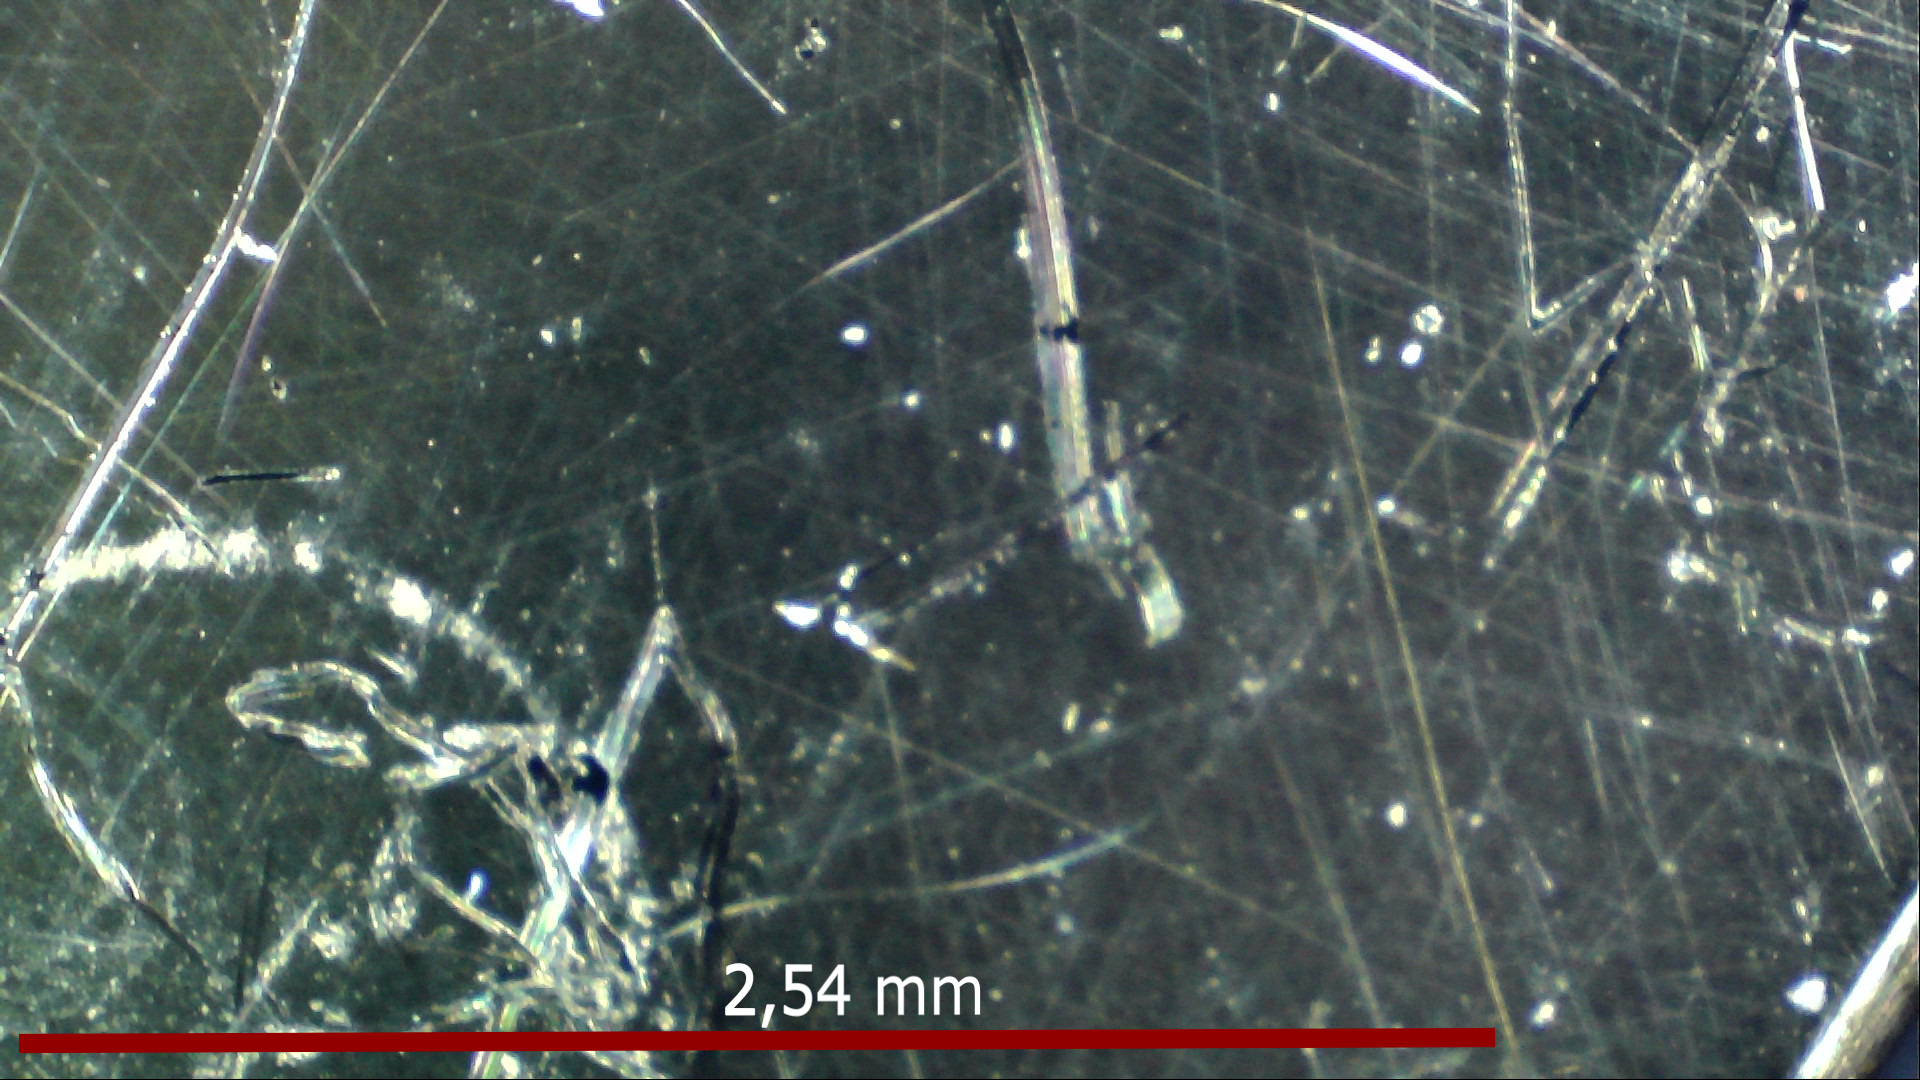
\includegraphics[width=\textwidth]{editgold_on_safir.png}
        \subcaption{Gold auf Saphir}
        \label{fig:golda}
    \end{minipage}
    \hfill
    \begin{minipage}[t]{0.495\textwidth}
        \centering
        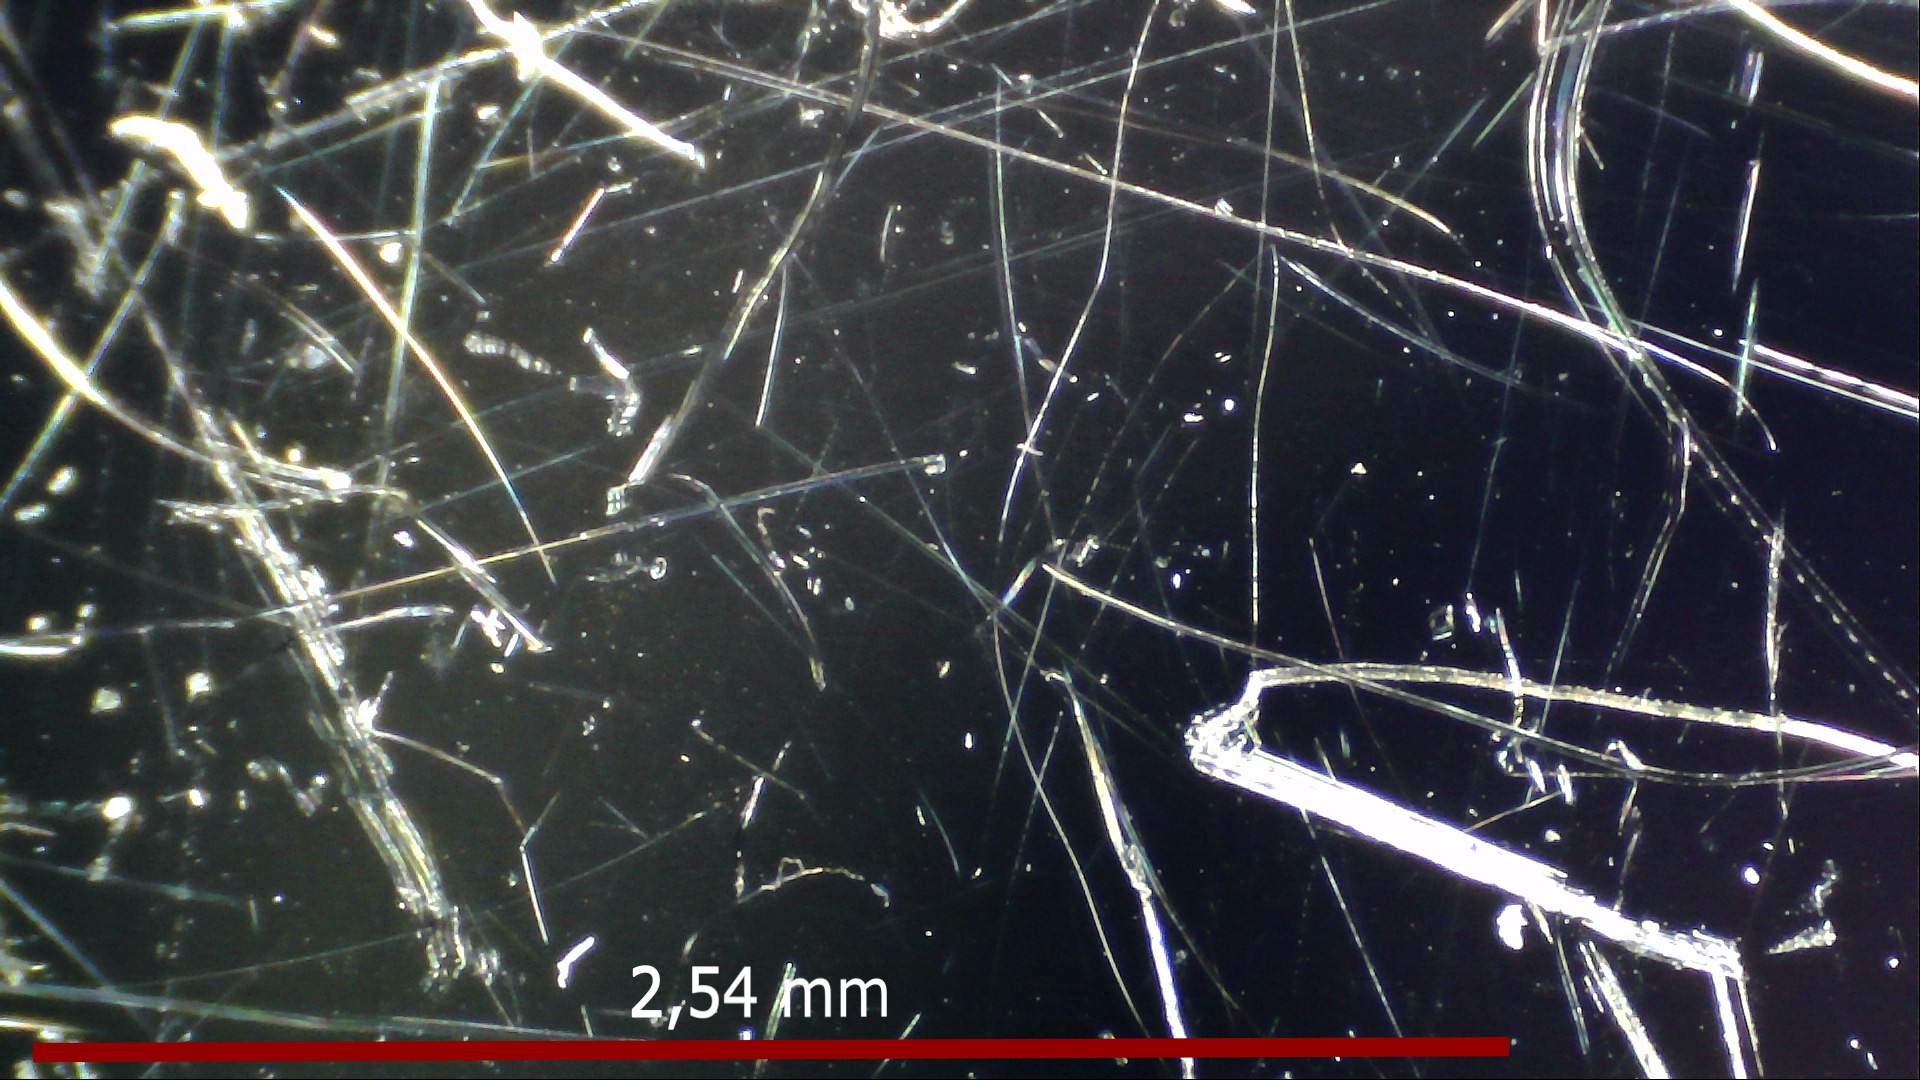
\includegraphics[width=\textwidth]{editgold_on_silizium.png}
        \subcaption{Gold auf Silizium}
        \label{fig:goldb}
    \end{minipage}
    \caption{Beide Goldproben unter dem USB-Mikroskop mit einer Linie der Länge $\SI{2.54}{\mm}$ als Maßstab.}
    \label{fig:gold_combined}
\end{figure}

Kratzer auf der Oberfläche lassen sich bereits in \cref{fig:gold_combined} mit dem USB-Mikroskop erkennen, deren Breite im Mikrometerbereich liegt. 
Sie stellen eine potenzielle Fehlerquelle dar: Kleinere Kratzer könnten so groß sein wie der künftige Bildausschnitt, weil das USB-Mikroskop nur die größten Kratzer erfasst. 
Wären die Kratzer größer, wäre dies kein Problem, da sie die lokal aufgezeichnete Struktur nicht beeinflussen würden. Ansonsten sind keine signifikanten Verunreinigungen oder zusätzlichen Oberflächenschäden feststellbar.

Nun beginnt die eigentliche Messung mit dem STM.
Die Spitze und die Probe werden in das STM eingesetzt, und zunächst wird ein Bild mit den Abmessungen $\SI{200}{\nm} \times \SI{200}{\nm}$ aufgenommen. 
Um die Scan-Geschwindigkeit zu berechnen, die einen Einfluss auf die Schärfe des aufgenommenen Bildes hat, muss die Bildlänge durch die vom Programm angegebene Geschwindigkeit dividiert werden. 
Dies ist darauf zurückzuführen, dass die vom Programm bereitgestellte Geschwindigkeit in ''Time per Line'' angegeben ist, also der Zeit, die die Spitze benötigt, um eine Scanzeile zu durchfahren (d.h. einen horizontalen Durchgang über den Bildausschnitt).

\begin{figure}[H]
    \centering
    \begin{minipage}[t]{0.495\textwidth}
        \centering
        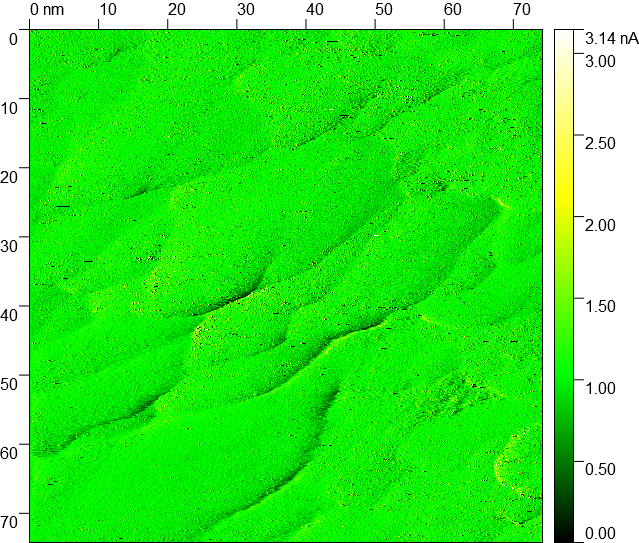
\includegraphics[width=\textwidth]{Au_Rund_useI.png}
        \label{fig:goldrund_I}
    \end{minipage}
    \hfill
    \begin{minipage}[t]{0.495\textwidth}
        \centering
        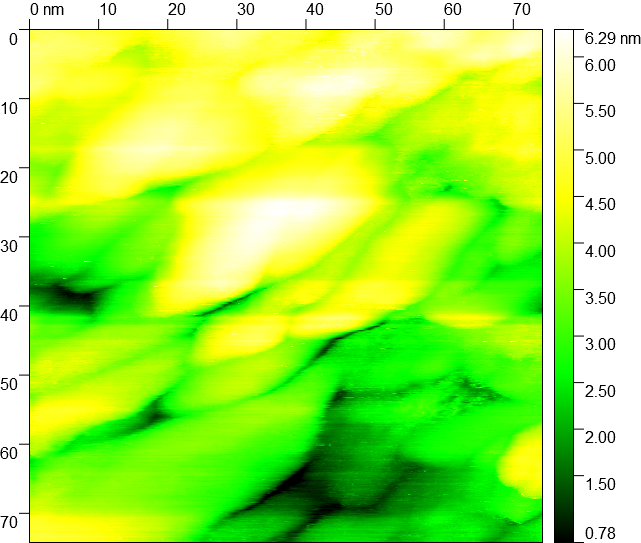
\includegraphics[width=\textwidth]{Au_Rund_useZ.png}
        \label{fig:goldrund_Z}
    \end{minipage}
    \caption{
      RTM-Aufnahme Gold auf Safir $\SI{74.2}{\nm}$; links: Tunnelstrom, rechts: Z-Achse; Setpoint $I = \SI{1}{\nano\ampere}$, Tip voltage $U = \SI{450}{\milli\volt}$,Rastergeschwindigkeit $v = \SI{185.5}{\nano\meter\per\second}$; $P = 1000$, $I = 2000$, $D = 0$
}
    \label{fig:goldrund_combined}
\end{figure}

\begin{figure}[H]
    \centering
    \begin{minipage}[t]{0.495\textwidth}
        \centering
        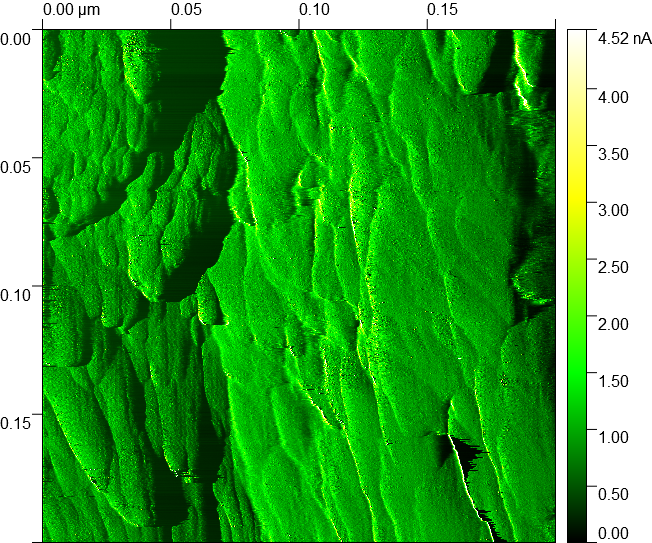
\includegraphics[width=\textwidth]{Au_Ecke_useI.png}
        \label{fig:goldecke_I}
    \end{minipage}
    \hfill
    \begin{minipage}[t]{0.495\textwidth}
        \centering
        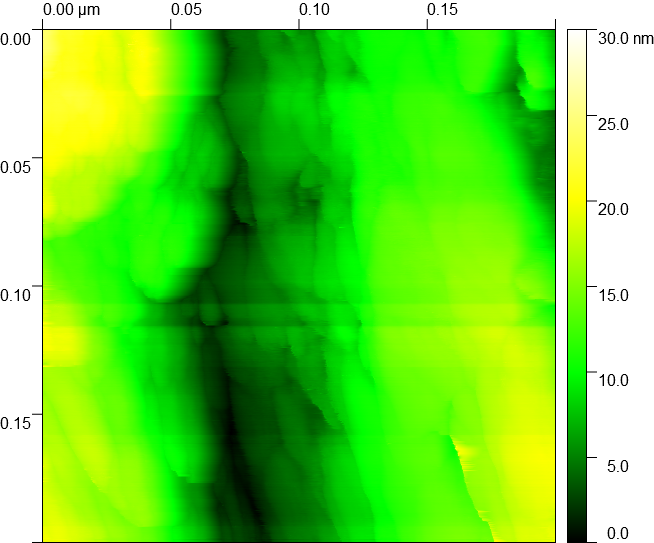
\includegraphics[width=\textwidth]{Au_Ecke_useZ.png}
        \label{fig:goldecke_Z}
    \end{minipage}
    \caption{
      RTM-Aufnahme Gold auf Silizium $\SI{200}{\nm}$; links: Tunnelstrom, rechts: Z-Achse; Setpoint $I = \SI{1}{\nano\ampere}$, Tip voltage $U = \SI{450}{\milli\volt}$,Rastergeschwindigkeit $v = \SI{500}{\nano\meter\per\second}$; $P = 1000$, $I = 2000$, $D = 0$
}
    \label{fig:goldecke_combined}
\end{figure}

Wie zu sehen ist, zeigen die Bilder tatsächlich eine raue Oberflächenstruktur in \cref{fig:goldecke_combined} und eine vergleichsweise glattere Oberflächenstruktur in \cref{fig:goldrund_combined}. 
In \cref{fig:goldecke_combined} deuten die starken Farbvariationen, die hier Höhenunterschiede repräsentieren, auf eine relativ rauere Oberfläche hin im Vergleich zu den schwachen Farbvariationen in \cref{fig:goldrund_combined}.


Dies spiegelt jedoch nicht notwendigerweise tatsächliche Höhenunterschiede in der Oberflächenstruktur wider, da das STM lediglich die Oberflächenladungsdichte detektiert und diese mit einer Höhe verknüpft. 
Da Gold ein Leiter ist, in dem sich Elektronen frei bewegen können, ist diese Verknüpfung nicht zwangsläufig physikalisch sinnvoll (bei metallischen Oberflächen Elektronendichte und wirkliche Topografie schwer zu trennen sind, da die Elektronen delokalisiert sind).

Wie zu erwarten stimmt die Gesamtstruktur des Materials (Sowohl \cref{fig:goldrund_combined} als auch \cref{fig:goldecke_combined}) sehr mit den in der Praktikumsanleitung \cite{praktikum} bereitgestellten Bildern überein.
Zudem sind wolkenartige Strukturen erkennbar, die, wie erwartet, das verdampfte Gold repräsentieren. 
Das Bild erscheint gelungen, da auf der rechten Seite nur eine scharfe Kante sichtbar ist, die höchstwahrscheinlich natürlichen Ursprungs und nicht auf eine unpräzise Oberflächenabtastung zurückzuführen ist. 
Ein Hinweis darauf ist, dass unter dem USB-Mikroskop bereits Kratzer im Mikrometerbereich beobachtet wurden, die in derselben Größenordnung wie der $\SI{2}{\micro\metre} \times \SI{2}{\micro\metre}$ Bildausschnitt liegen. 
Es ist daher wahrscheinlich, dass kleinere Kratzer ähnlicher Größe existieren, die mit dem USB-Mikroskop nicht sichtbar waren.


Bei \cref{fig:goldecke_combined} sind die Farbvariationen vergleichsweise minimal, und die wenigen Anomalien lassen sich auf Kratzer und zerbrochene Segmente zurückführen, die aufgrund der begrenzten Auflösung des USB-Mikroskops zu klein sind, um eindeutig dargestellt zu werden.


Da das STM bei Gold ohne Absturz arbeitete und repräsentative Topografien lieferte, folgt nun die Untersuchung der anspruchsvolleren HOPG-Probe.

 \chapter{HOPG-Probe}
%Bevor die HOPG-Probe mit atomarer Auflösung analysiert werden kann, wird ihre grobe Oberflächenstruktur zunächst mit einem USB-Lichtmikroskop untersucht. Abbildung !!!ADDREF!!!! zeigt den Zustand der Probe (HOPG) nach dem Entfernen einer Schicht. Es ist zu erkennen, dass die oberste Graphitschicht keine gleichmäßig ebene Oberfläche aufweist, sondern aus mehreren plattenartigen Segmenten besteht, die in unterschiedlichen Winkeln zueinander ausgerichtet sind. Dies wird durch die unterschiedlichen Reflexionswinkel der einzelnen Bereiche deutlich.

%Um eine möglichst glatte Oberfläche für die Analyse mit einem Rastertunnelmikroskop zu erzeugen, wird die oberste Graphitschicht erneut mit Klebeband entfernt. Nach dieser Behandlung erscheint die Probe optisch glatt, das mit dem USB-Mikroskop aufgenommene Bild !!!!ADDREF!!! zeigt jedoch noch eine gewisse Segmentierung (!!!!!CONFIRM OR NOT THIS OBSERVATION!!!!). Für RTM-Untersuchungen ist jedoch nur eine ebene Oberfläche über wenige Quadratnanometer erforderlich, sodass der hergestellte Zustand als ausreichend geeignet gilt.

%Im nächsten Schritt wird die HOPG-Probe in den Probenhalter des Rastertunnelmikroskops eingesetzt. Zusätzlich wird eine neue Spitze für die Untersuchung vorbereitet und in die dafür vorgesehene Klemme des STM eingesetzt. Eine vergrößerte Abbildung der Spitze ist in Abbildung !!!!ADDREF!!! dargestellt.


%Nach erfolgreicher Positionierung von Probe und Spitze erfolgt die Annäherung zunächst mit "advance" und anschließend mit "approach". Sobald die Steuerelektronik den Tunnelkontakt registriert, kann die Messung gestartet werden. Es wurden mehrere Bilder mit unterschiedlichen Vergrößerungen aufgenommen.

%Das RTM wurde zunächst im "constant current mode" betrieben, um Kollisionen der Spitze mit möglichen Oberflächenunebenheiten zu vermeiden. Der "constant height mode" wurde später für hochauflösende Detailbilder auf atomarer Ebene verwendet.

%Abbildung !!!ADDREF!!! zeigt ein Bild einer Graphitoberfläche mit einem Raster von !!!ADDSCALING!!! Kantenlänge. Da es im "constant current mode" aufgenommen wurde, enthält das Höhenbild !!!WHERE!!! topografische Informationen. Der dargestellte Ausschnitt zeigt drei weitgehend planare Segmente der Graphitoberfläche, die bereits im Lichtmikroskopbild makroskopisch sichtbar waren !!!ADDREF!!!. Ihre Kanten sind scharf, was im Strombild !!!WHERE!!! besonders deutlich wird, da der PID-Regler eine schnelle Änderung des Tunnelstroms erfasste. Insgesamt zeigt das Strombild, dass der Regelkreis einen weitgehend konstanten Tunnelstrom aufrechterhält, was auf eine präzise Einstellung der Regelparameter hindeutet. !!!CONFIRM/DENYOBSERVATION!!!

%Das Höhenbild in !!!ADDREF!!! zeigt deutlich, dass der zu beobachtende Probenbereich für die atomare Auflösung geeignet ist, da das zentrale Segment eine nahezu flache Struktur im Nanometerbereich aufweist.!!!CONFIRM/DENYOBSERVATION!!! 

%Zur Bestätigung !!!DIDWEDOTHAT???!!!!!! wurde zusätzlich ein kleineres Ausschnittsbild von !!!!ADDSCALING!!! aufgenommen. Das Ergebnis dieser Messung ist in !!!!ADDREF!!!! dargestellt.

%Es gibt keine größeren Unregelmäßigkeiten im gescannten Gebiet. Lediglich vereinzelte Abweichungen vom Mittelwert sind sowohl im Höhenbild als auch im Strömungsbild erkennbar. Zur quantitativen Analyse ist die Verteilungsfunktion der Höhenwerte in !!!ADDREF-HÖHENPROFIL!!! dargestellt. Die Daten können durch eine Gauß-Funktion mit Mittelwert !!!!!!!!!!ADD-PARAMETERS-GAUSSFIT mu =  und Standardabweichung sigma= !!!!!!!!!!!! modelliert werden.

%Da der Bereich \( \sigma \) sehr klein ist, kann angenommen werden, dass die Aufnahme im "constant height mode" durchgeführt werden kann, ohne die Spitze oder die Probe zu beschädigen. Um in diesen Modus zu wechseln, wird der PID-Regler mit den Parametern P = 0, I = 4, D = 0 eingestellt.

%Die nächste Aufnahme wird mit einer Scanbreite von !!!!ADDSCALE!!!!!! durchgeführt. Abbildung !!!!ADDREF!!!!! zeigt die entsprechenden Messergebnisse des RTM. Da in dieser Aufnahme der "constant height mode" verwendet wurde, enthält das aktuelle Bild nun topografische Informationen. Das Höhenbild zeigt nur Stellen, an denen die feste Komponente des PID-Reglers kleine Höhenanpassungen vorgenommen hat, um große Bodenunebenheiten oder Gefälle.

%!!!!ADD PICS AND COMMENTS EXPLAINING THAT YOU CAN'T SEE SHIT AND MAYBE SOME PICS OF WHAT IT SHOULD LOOK LIKE THEORETICALLY AND HOW WE WOULD DETERMINE THE ANGLE AND THE DISTANCE WITH GOOD PICS!!!!!!


 \chapter{Fazit}
In diesem Experiment wurde der Umgang mit einem Rastertunnelmikroskop erfolgreich erlernt. Eine Goldprobe und eine HOPG-Probe wurden analysiert. Ziel der Untersuchung der Goldprobe war die Erstellung hochwertiger Bilder, die die Oberflächenstruktur der Probe detailliert beschreiben – ein Ziel, das erfolgreich erreicht/nicht erfolgreich erreicht wurde. Anschließend wurde die HOPG-Probe analysiert, bei welchen eine atomare Auflösung erreicht werden sollte. Diese Analyse verlief erfolgreich/nicht erfolgreich, sodass die durchschnittlichen Bindungswinkel und Atomabstände der Kohlenstoffatome aus den erhaltenen Bildern bestimmt werden konnten/nur annähernd bestimmt werden konnten.
Die Messungen ergaben einen durchschnittlichen Bindungswinkel von ( ± )° und einen durchschnittlichen Atomabstand von ( ± ) [Einheit]. Obwohl der ermittelte Bindungswinkel weitgehend mit den Literaturwerten übereinstimmt/nicht übereinstimmt, weist der durchschnittliche Atomabstand eine signifikante/kleine Abweichung auf. Eine mögliche Fehlerquelle ist eine ungenaue Kalibrierung der Piezoelemente im STM. Eine perspektivische Verzerrung, die durch die Neigung der Gitterebene der Probe verursacht wird, könnte ebenfalls zu Abweichungen geführt haben. Daher sind zusätzliche Kalibrierungsmessungen mit dem Gerät erforderlich, um die Genauigkeit der Ergebnisse zu verbessern.
 \chapter{Formeln: To be deleted at the end}

\section*{Spannungsteiler}

\begin{equation}
  U = \frac{R_2}{R_1 + R_2}\,U_{\mathrm{ges}}
\end{equation}

mit $U$ als Spannung am Widerstand $R_2$, $R_1$ und $R_2$ als Widerstände und $U_{\mathrm{ges}}$ als Gesamtspannung.

\section*{Energieerhaltung}

\begin{equation}
  h\,f = E_{\mathrm{kin}} + W_A,
  \quad
  E_{\mathrm{kin}} = e\,U_G
\end{equation}

mit $h$ dem Planckschen Wirkungsquantum, $f$ der Photonfrequenz, $e$ der Elementarladung, $U_G$ der Gegenspannung und $W_A$ der Austrittsarbeit.

\section*{Fehlerfortpflanzung I}

\begin{equation}
  \Delta\bigl(\sqrt{I - I_0}\bigr)
  = \sqrt{
    \Bigl(\tfrac{\Delta I}{2\,\sqrt{I - I_0}}\Bigr)^{2}
   +\Bigl(\tfrac{\Delta I_0}{2\,\sqrt{I - I_0}}\Bigr)^{2}
  }.
\end{equation}

\section*{Beugungsgitter}

\begin{equation}
  g\bigl(\sin\theta_m + \sin\beta\bigr) = m\,\lambda
  \quad\Longrightarrow\quad
  g = \frac{m\,\lambda}{\sin\theta_m + \sin\beta}
\end{equation}

\begin{equation}
  \Delta g
  = \sqrt{
    \Bigl(\tfrac{\partial g}{\partial\theta_m}\,\Delta\theta_m\Bigr)^{2}
   +\Bigl(\tfrac{\partial g}{\partial\beta}\,\Delta\beta\Bigr)^{2}
  }.
\end{equation}

\begin{equation}
  \frac{\partial g}{\partial\theta_m}
  = \frac{m\,\lambda\,\cos\theta_m}{(\sin\theta_m + \sin\beta)^{2}},
  \quad
  \frac{\partial g}{\partial\beta}
  = \frac{m\,\lambda\,\cos\beta}{(\sin\theta_m + \sin\beta)^{2}}.
\end{equation}

\section*{Mittelwert der Gitterkonstante}

\begin{equation}
  \overline{g}
  = \frac{\sum_{i=1}^{N} \bigl(g_i/\Delta g_i\bigr)}
         {\sum_{i=1}^{N} \bigl(1/\Delta g_i\bigr)},
  \quad
  \Delta\overline{g}
  = \sqrt{\frac{N}{\sum_{i=1}^{N} 1/(\Delta g_i)^{2}}}\,.
\end{equation}

\section*{Isotopenverhältnis}

\begin{equation}
  \lambda = g\,(\sin\theta_m + \sin\beta),
  \quad
  \frac{\partial\lambda}{\partial\beta} = g\,\cos\beta,
  \quad
  \Delta\beta \approx \frac{d}{f}.
\end{equation}

\section*{Fehlerfortpflanzung II}

\begin{equation}
  \Delta\lambda
  = \sqrt{
      \Bigl(\tfrac{\lambda}{g}\,\Delta g\Bigr)^{2}
    + \Bigl(g\,\cos\alpha\,\Delta\alpha\Bigr)^{2}
    + \Bigl(g\,\cos\beta\,\Delta\beta\Bigr)^{2}
  }.
\end{equation}

\begin{equation}
  \Delta(\Delta\lambda)
  = \sqrt{
      \Bigl(\tfrac{d\,\cos\beta}{f}\,\Delta g\Bigr)^{2}
    + \Bigl(\tfrac{-d\,\sin\beta}{f\,g}\,\Delta\beta\Bigr)^{2}
    + \Bigl(\tfrac{g\,\cos\beta}{f}\,\Delta d\Bigr)^{2}
  }.
\end{equation}

\section*{Balmer‐Formel}

\begin{equation}
  \frac{1}{\lambda}
  = R_H\Bigl(\tfrac{1}{2^{2}} - \tfrac{1}{n^{2}}\Bigr),
  \quad n=3,4,5,\dots
\end{equation}

\begin{equation}
  R_H
  = \frac{1/\lambda}{\bigl(\tfrac{1}{4} - \tfrac{1}{n^{2}}\bigr)},
  \quad
  \Delta R_H
  = \frac{\Delta\lambda}{\lambda^{2}\,\bigl(\tfrac{1}{4} - \tfrac{1}{n^{2}}\bigr)}.
\end{equation}

\section*{Plancksches Wirkungsquantum}

\begin{equation}
  h
  = \Bigl(\tfrac{m_e\,e^{4}}{8\,\varepsilon_{0}^{2}\,c\,R_H}\Bigr)^{1/3},
  \quad
  \Delta h
  = \frac{1}{3}
    \Bigl(\tfrac{m_e\,e^{4}}{8\,\varepsilon_{0}^{2}\,c}\Bigr)^{1/3}
    R_H^{-4/3}\,\Delta R_H.
\end{equation}


\appendix
\printbibliography{}
\listoffigures\addcontentsline{toc}{chapter}{Abbildungsverzeichnis}
\listoftables\addcontentsline{toc}{chapter}{Tabellenverzeichnis}
 \chapter{Anhang}
\section{Abbildungen}
\subsection*{Photoeffekt}
\subsection*{Balmer Serie}

\begin{figure}[H]
\centering
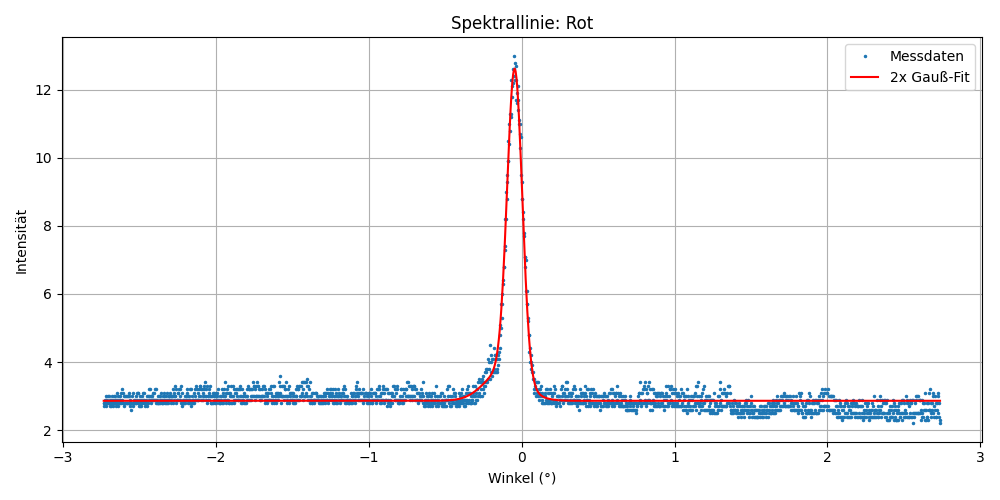
\includegraphics[width=0.7\linewidth]{figs/dt_rot_155_62.png}
\caption{Gaußfit für $H_\alpha$ mit $\chi_{red} = 0.06$}
\label{fig:H_a}
\end{figure}

\begin{figure}[H]
\centering
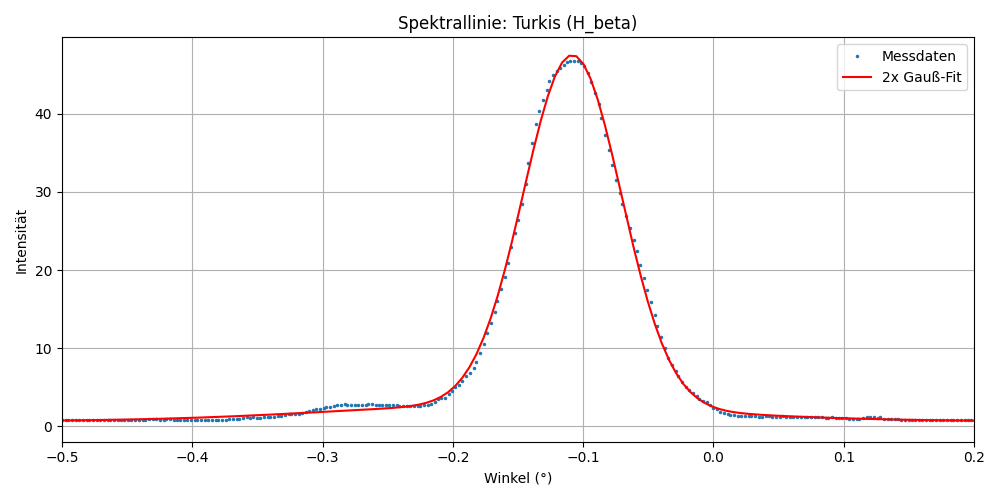
\includegraphics[width=0.7\linewidth]{figs/dt_turkis_145_55_5.png}
\caption{Gaußfit für $H_\beta$ mit $\chi_{red} = 0.06$}
\label{fig:H_b}
\end{figure}

\begin{figure}[H]
\centering
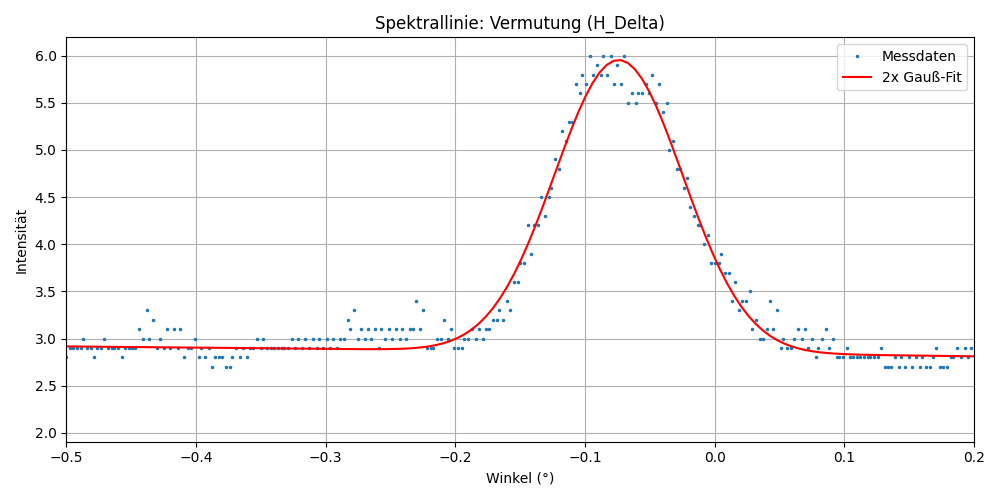
\includegraphics[width=0.7\linewidth]{figs/dt_vermutung_145_49.png}
\caption{Gaußfit für die Vermutete Linie $H_\delta$ mit $\chi_{red} = 0.03$}
\label{fig:H_d}
\end{figure}


\begin{figure}[H]
  \centering
  \begin{minipage}[t]{\textwidth}
    \centering
    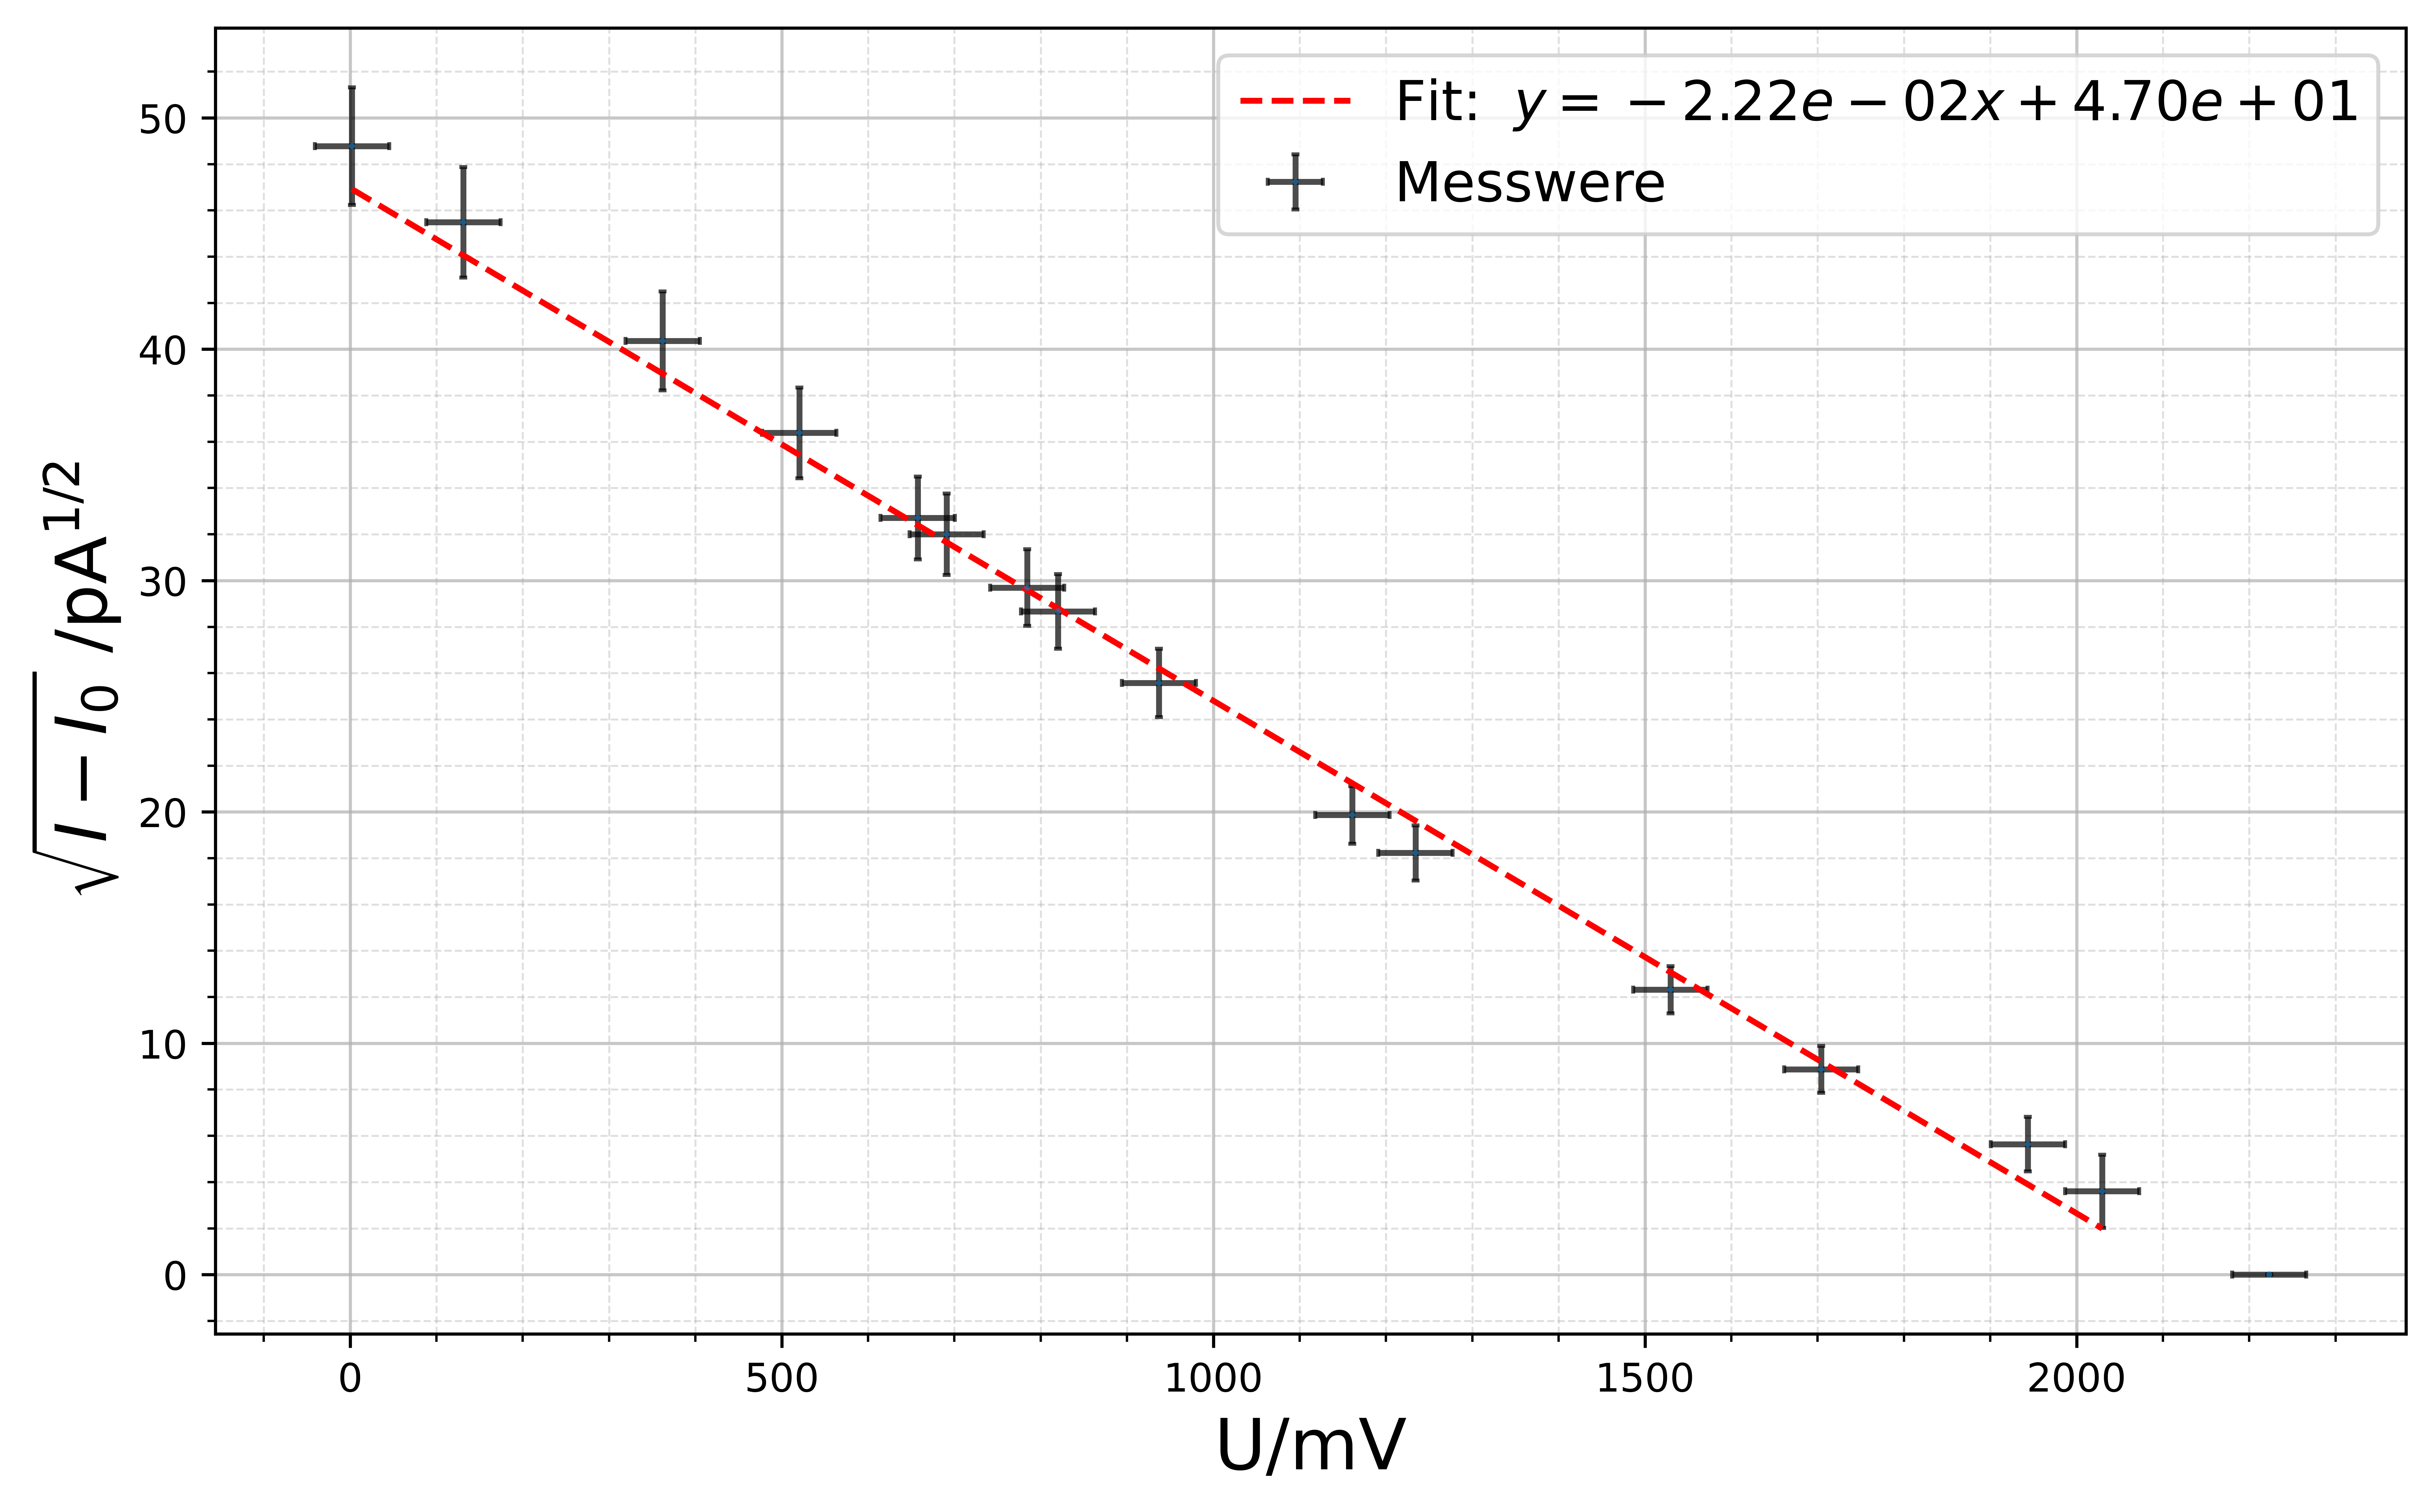
\includegraphics[width=0.95\linewidth]{figs/365_1.png}
    \captionof{figure}{Messung 1 bei $\lambda=\SI{365}{\nm}$. Die Werte und Unsicherheiten sind in ~\cref{tab:365_first}.}
    \label{fig:365_first}
  \end{minipage}\hfill
  \begin{minipage}[t]{\textwidth}
    \centering
    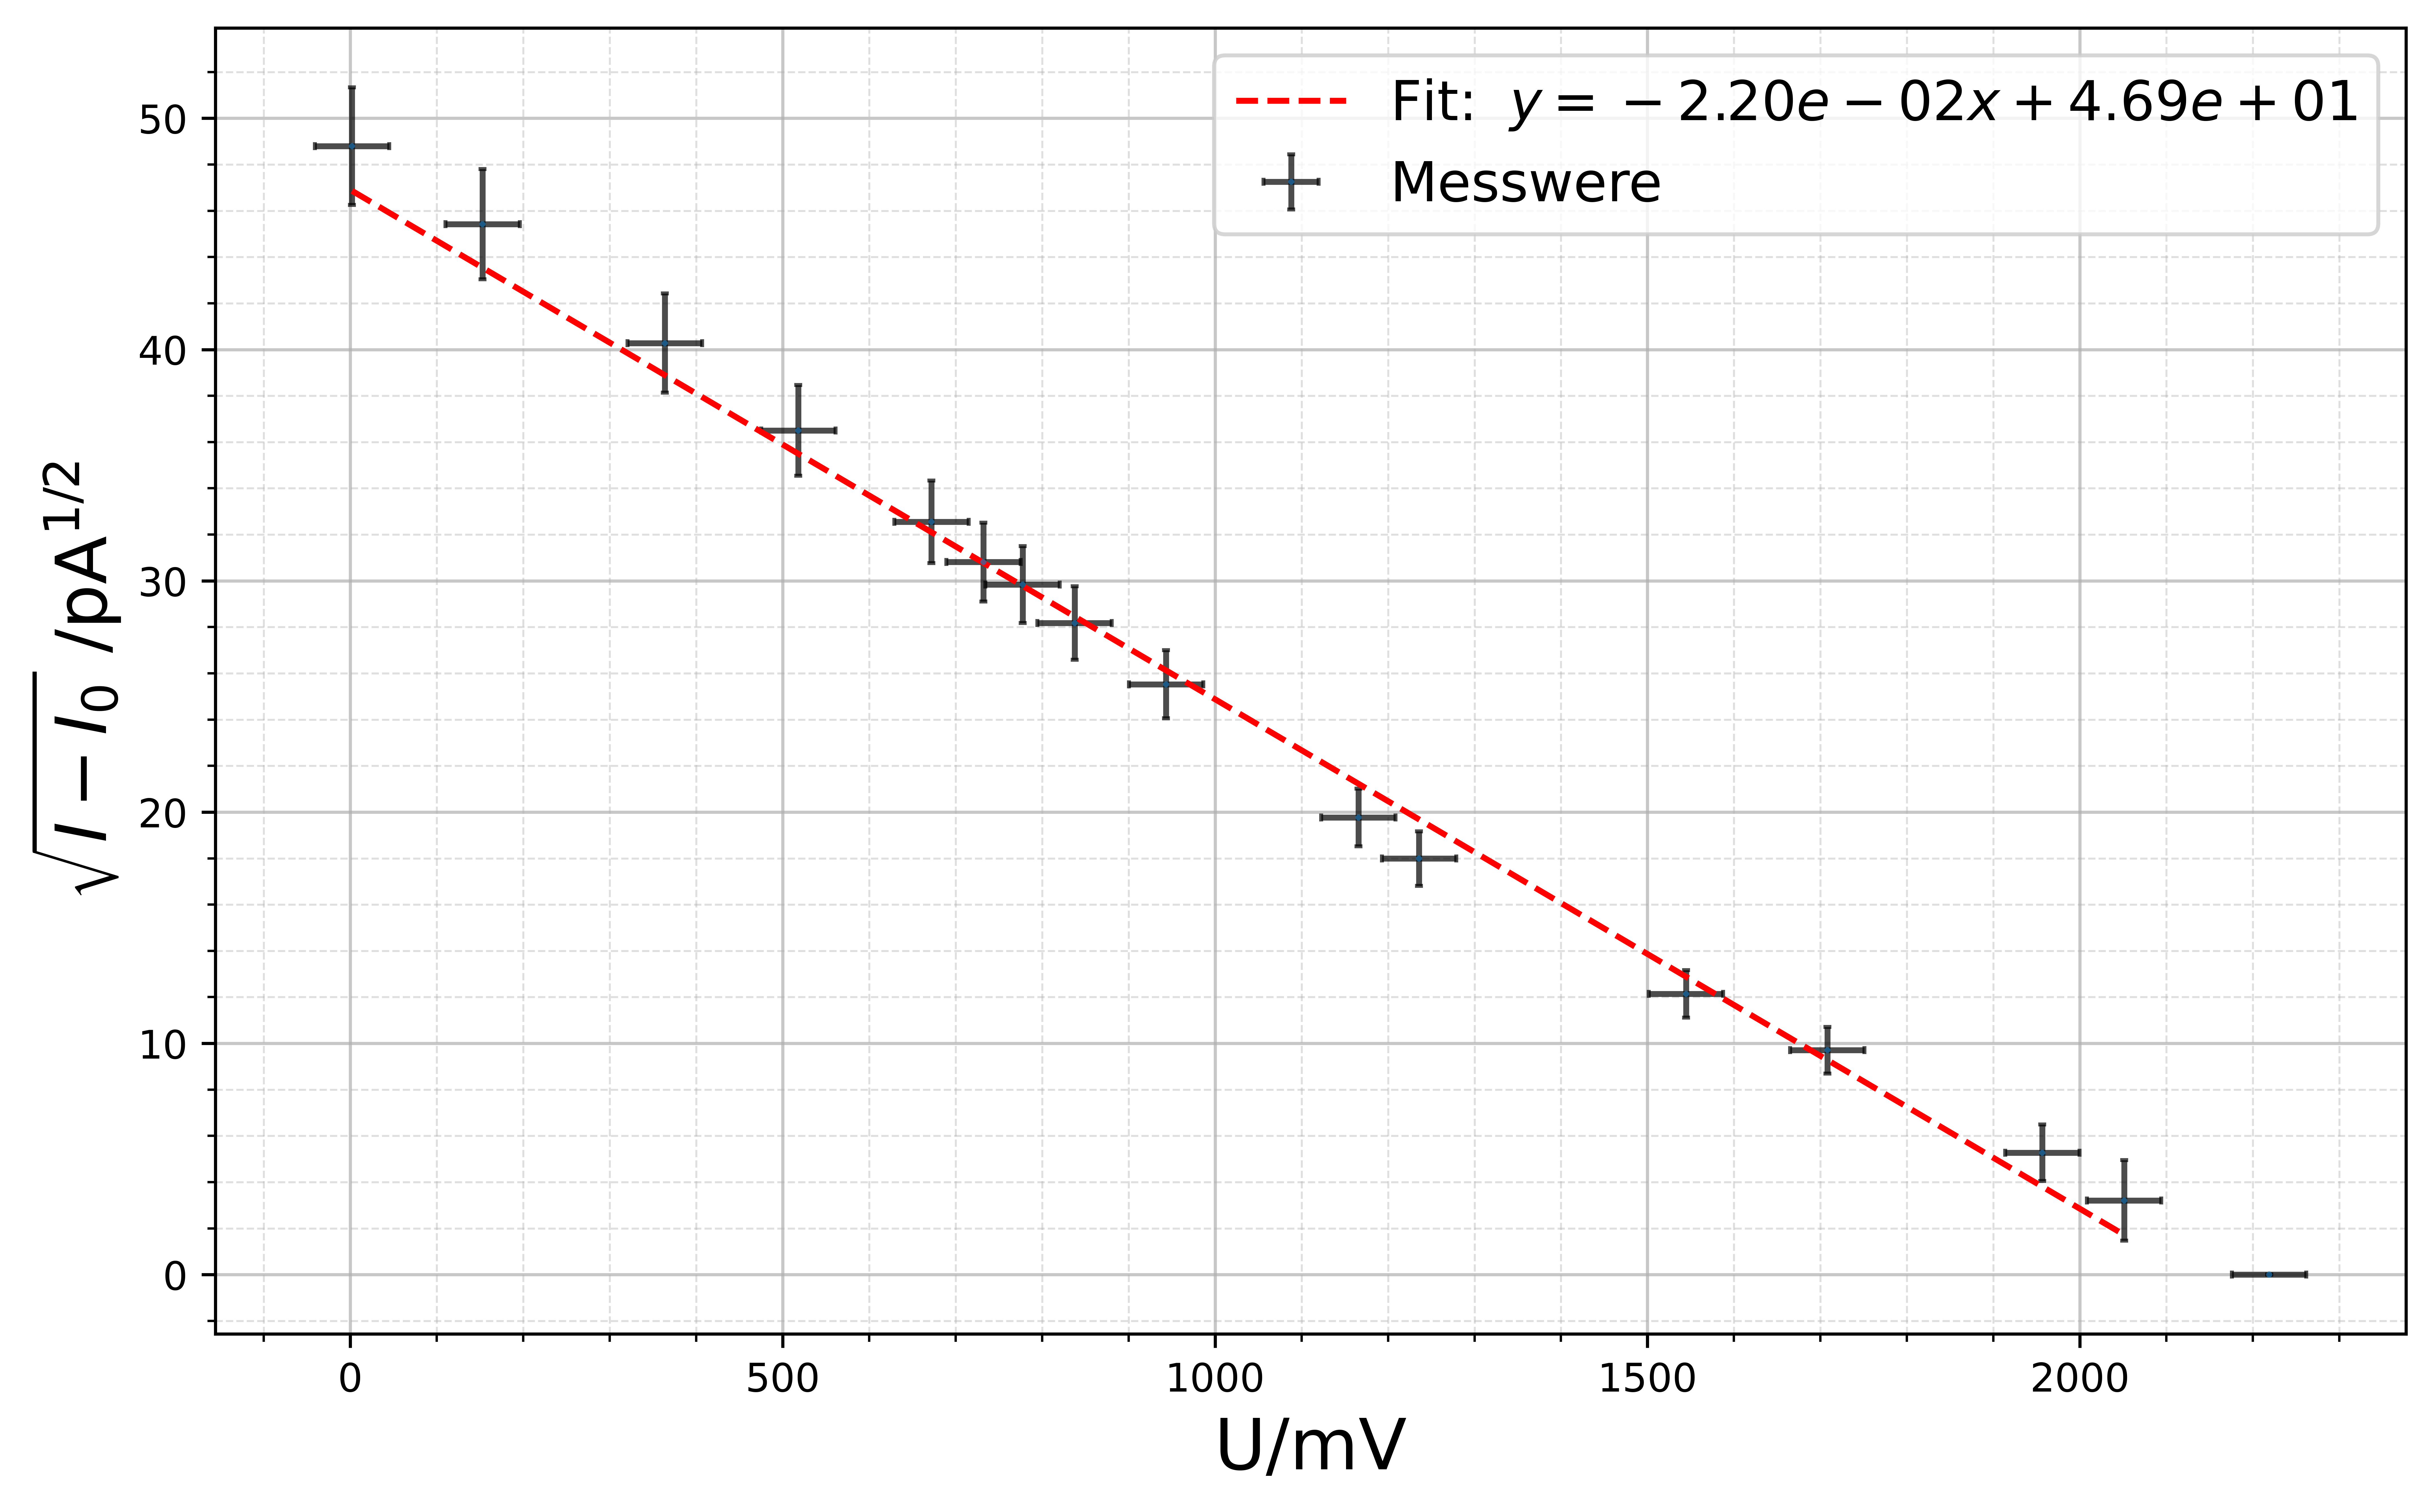
\includegraphics[width=0.95\linewidth]{figs/365_2.png}
    \captionof{figure}{Messung 2 bei $\lambda=\SI{365}{\nm}$. Die Werte und Unsicherheiten sind in ~\cref{tab:365_second}.}
    \label{fig:365_second}
  \end{minipage}\hfill
\end{figure}
\vfil
\begin{figure}[H]
  \centering
  \begin{minipage}[t]{\linewidth}
    \centering
    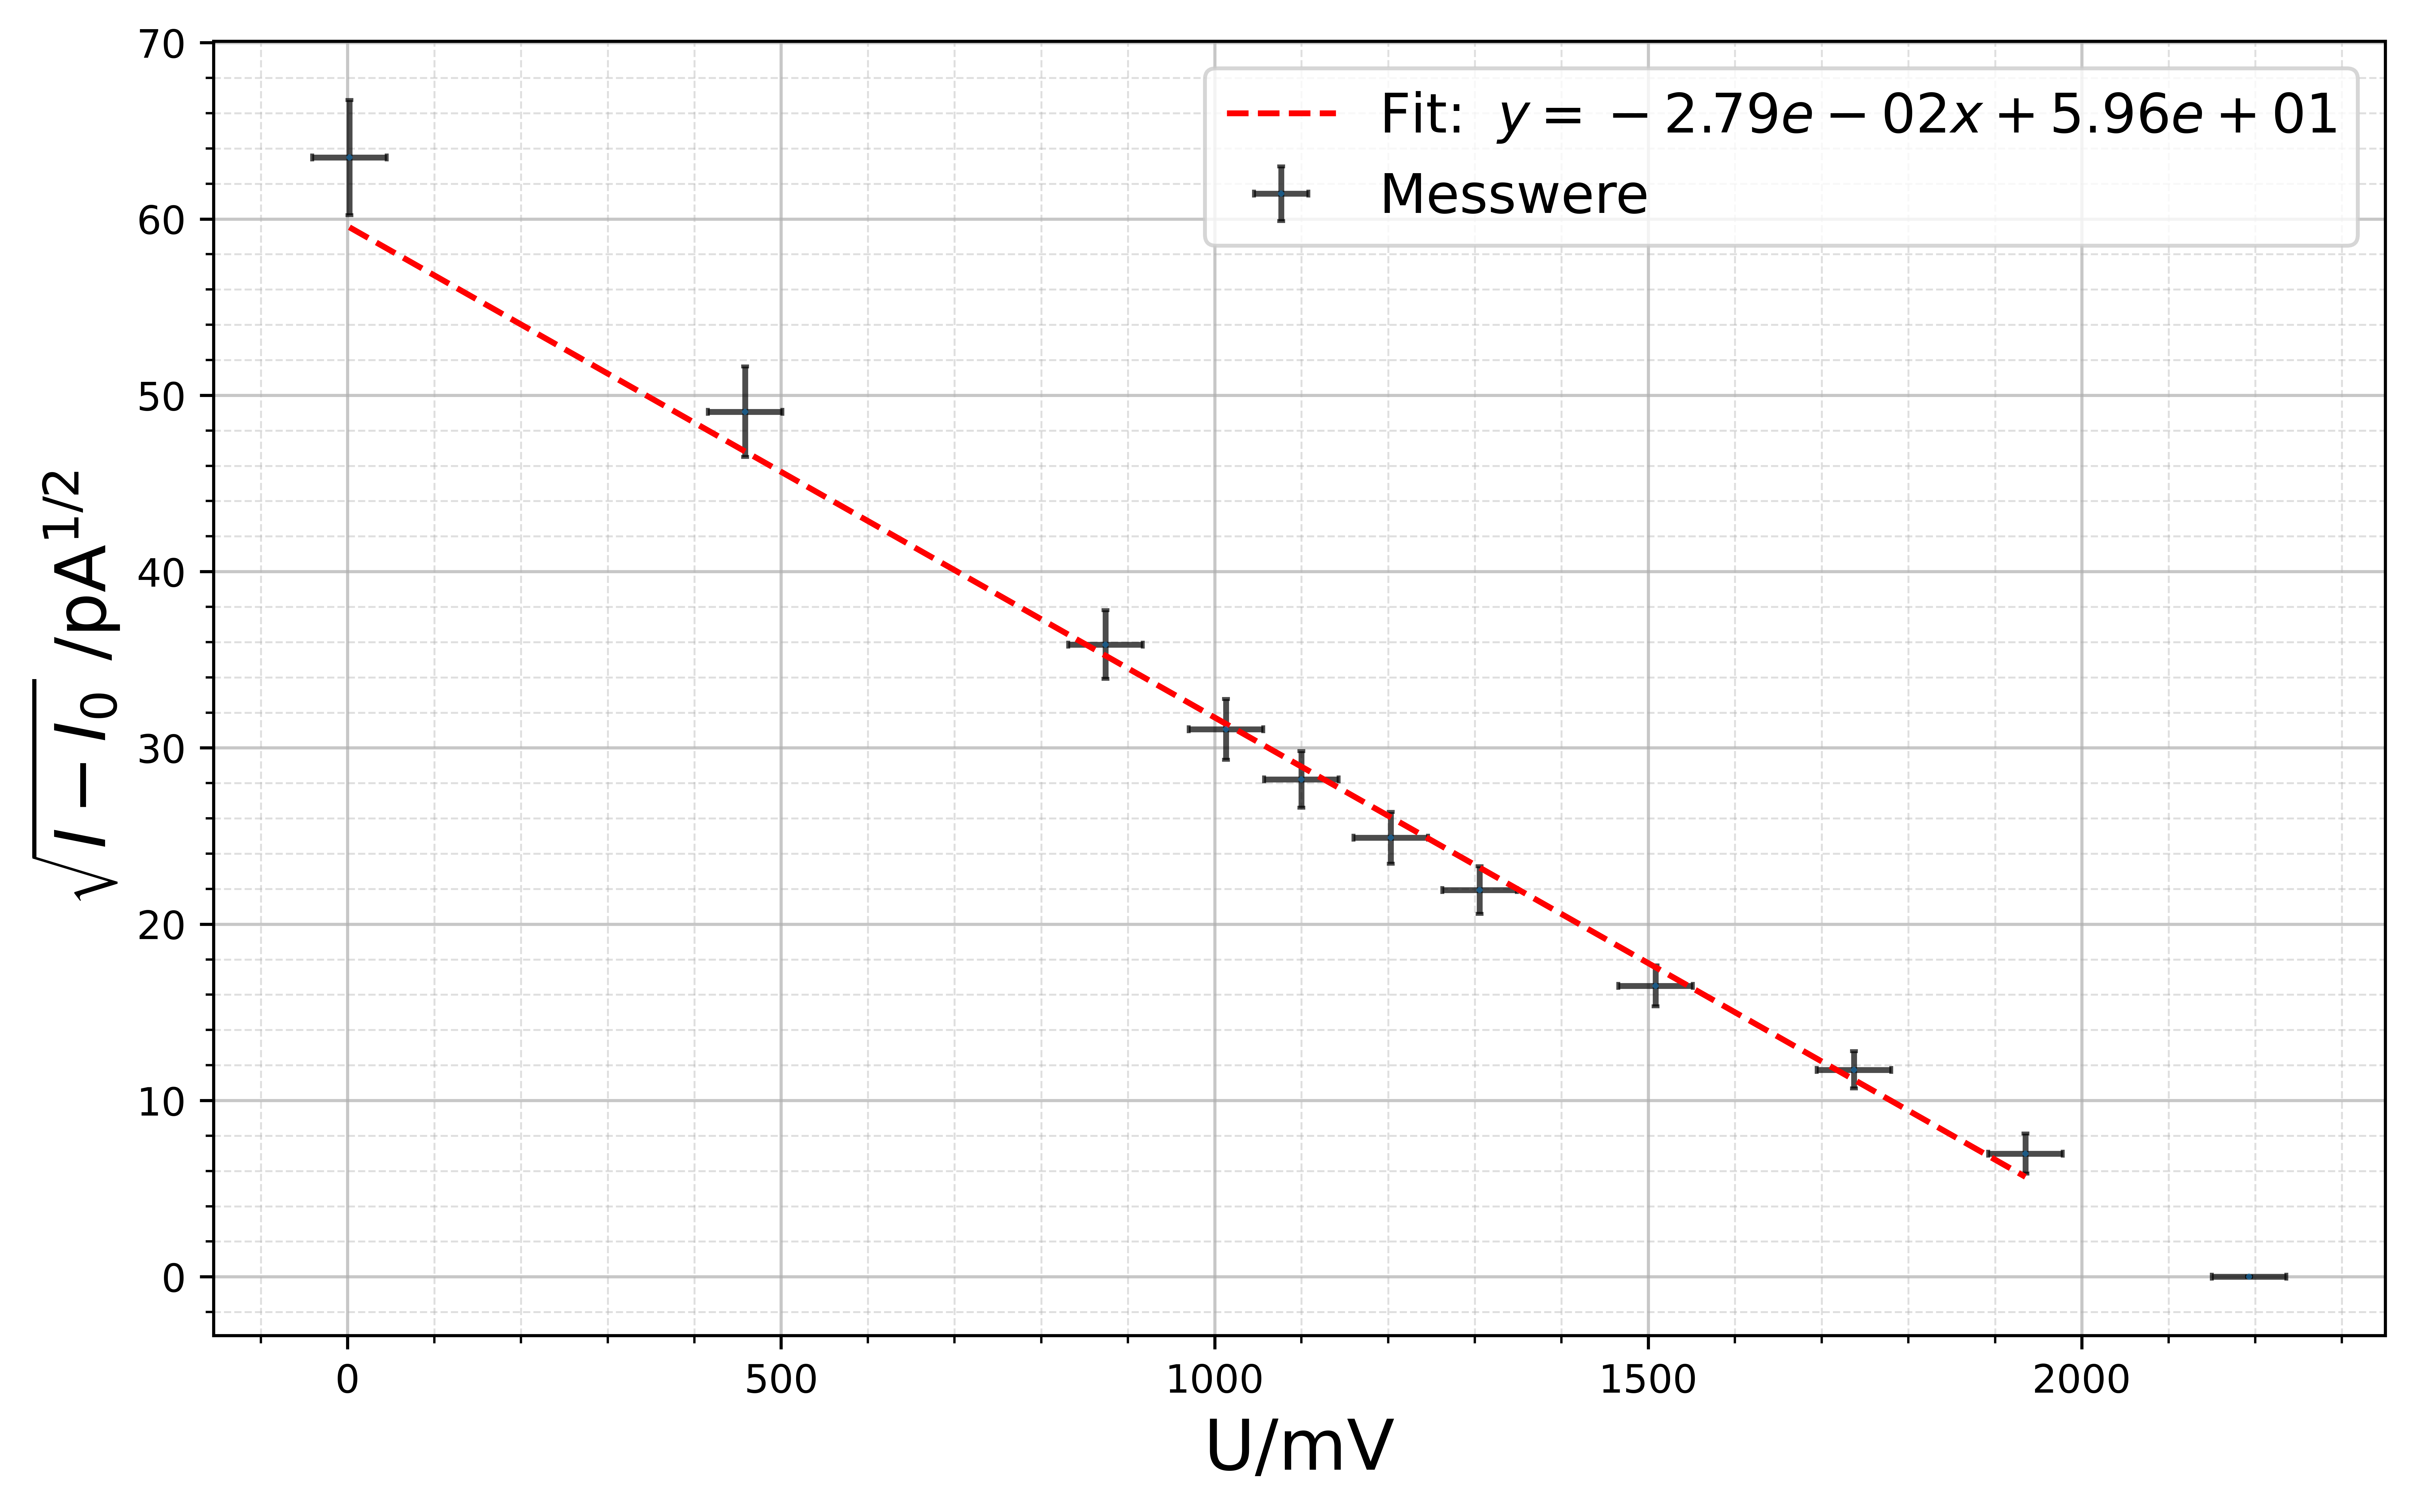
\includegraphics[width=0.95\linewidth]{figs/365_50.png}
    \captionof{figure}{Messung bei $50\%$ Intensität und $\lambda=\SI{365}{\nm}$. 
    Die Werte und Unsicherheiten sind in \cref{tab:365_50pct}.%
    }
    \label{fig:365_50}
  \end{minipage}\hfill
  \begin{minipage}[t]{\linewidth}
    \centering
    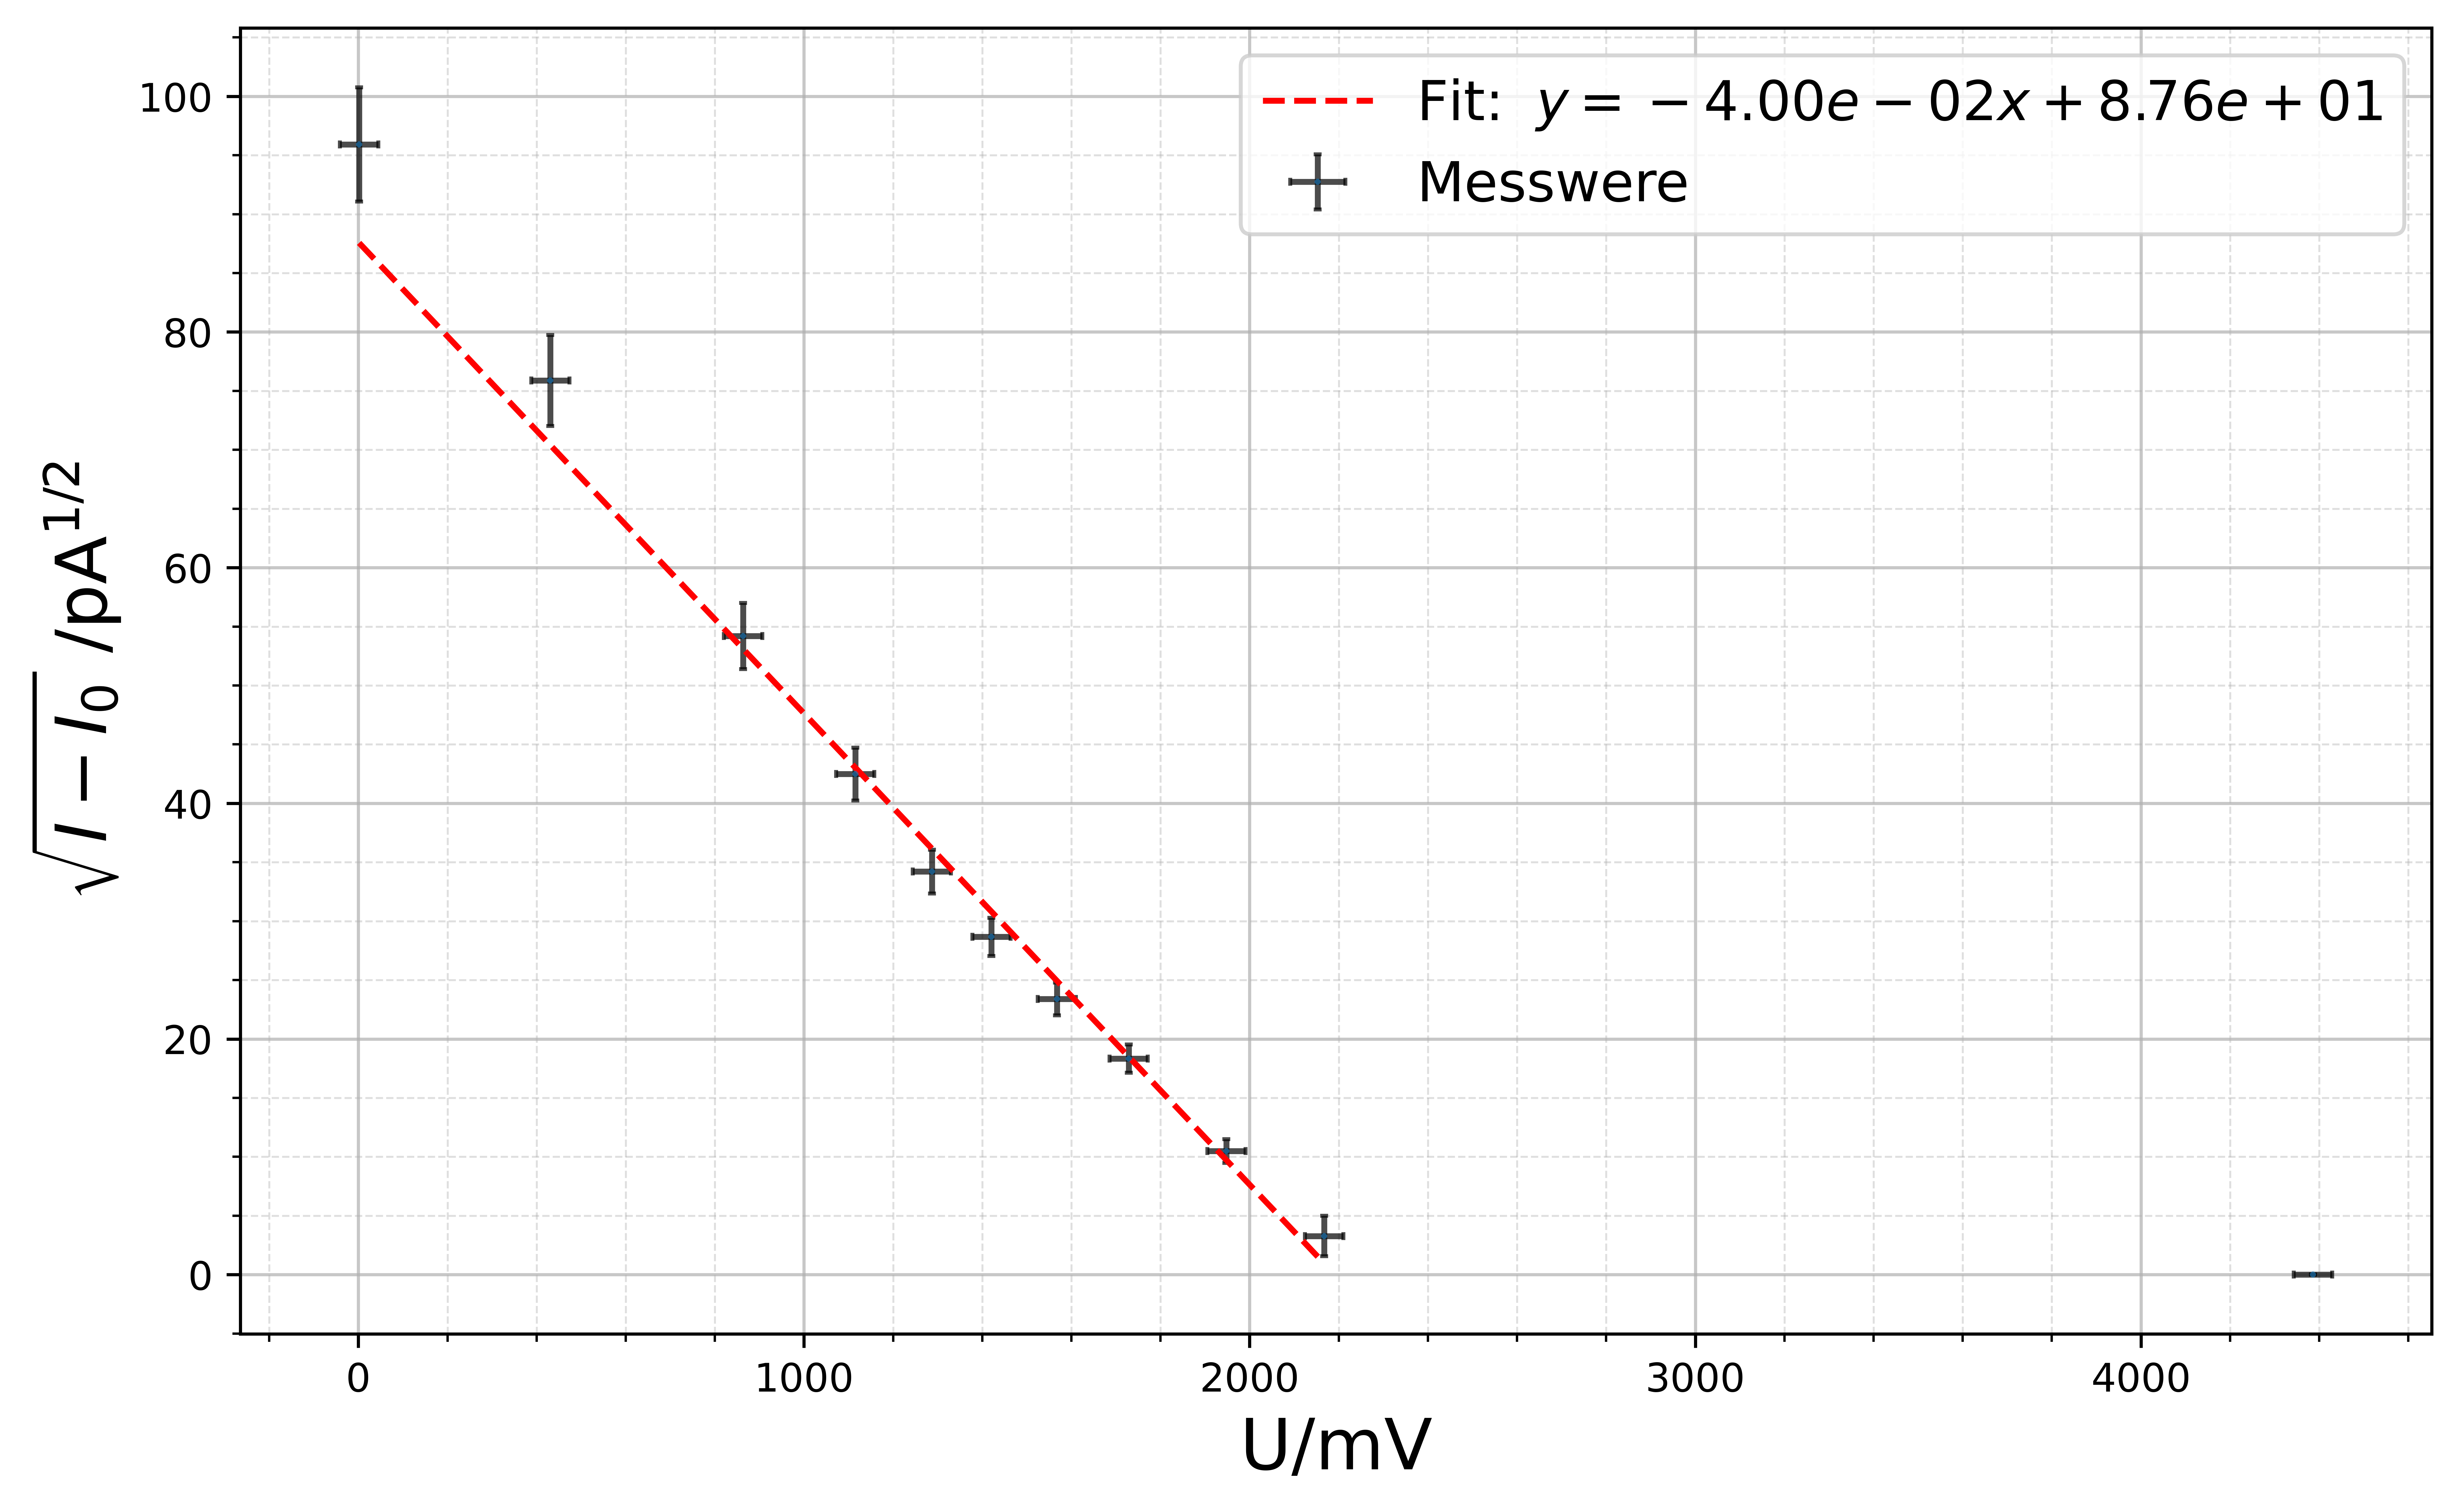
\includegraphics[width=0.95\linewidth]{figs/365_max.png}
    \captionof{figure}{%
      Messung bei maximaler Intensität und $\lambda=\SI{365}{\nm}$. 
      Die Werte und Unsicherheiten sind in \cref{tab:365_max}.%
    }
    \label{fig:365_max}
  \end{minipage}
\end{figure}

\begin{figure}[H]
  \centering
  \begin{minipage}[t]{\linewidth}
    \centering
    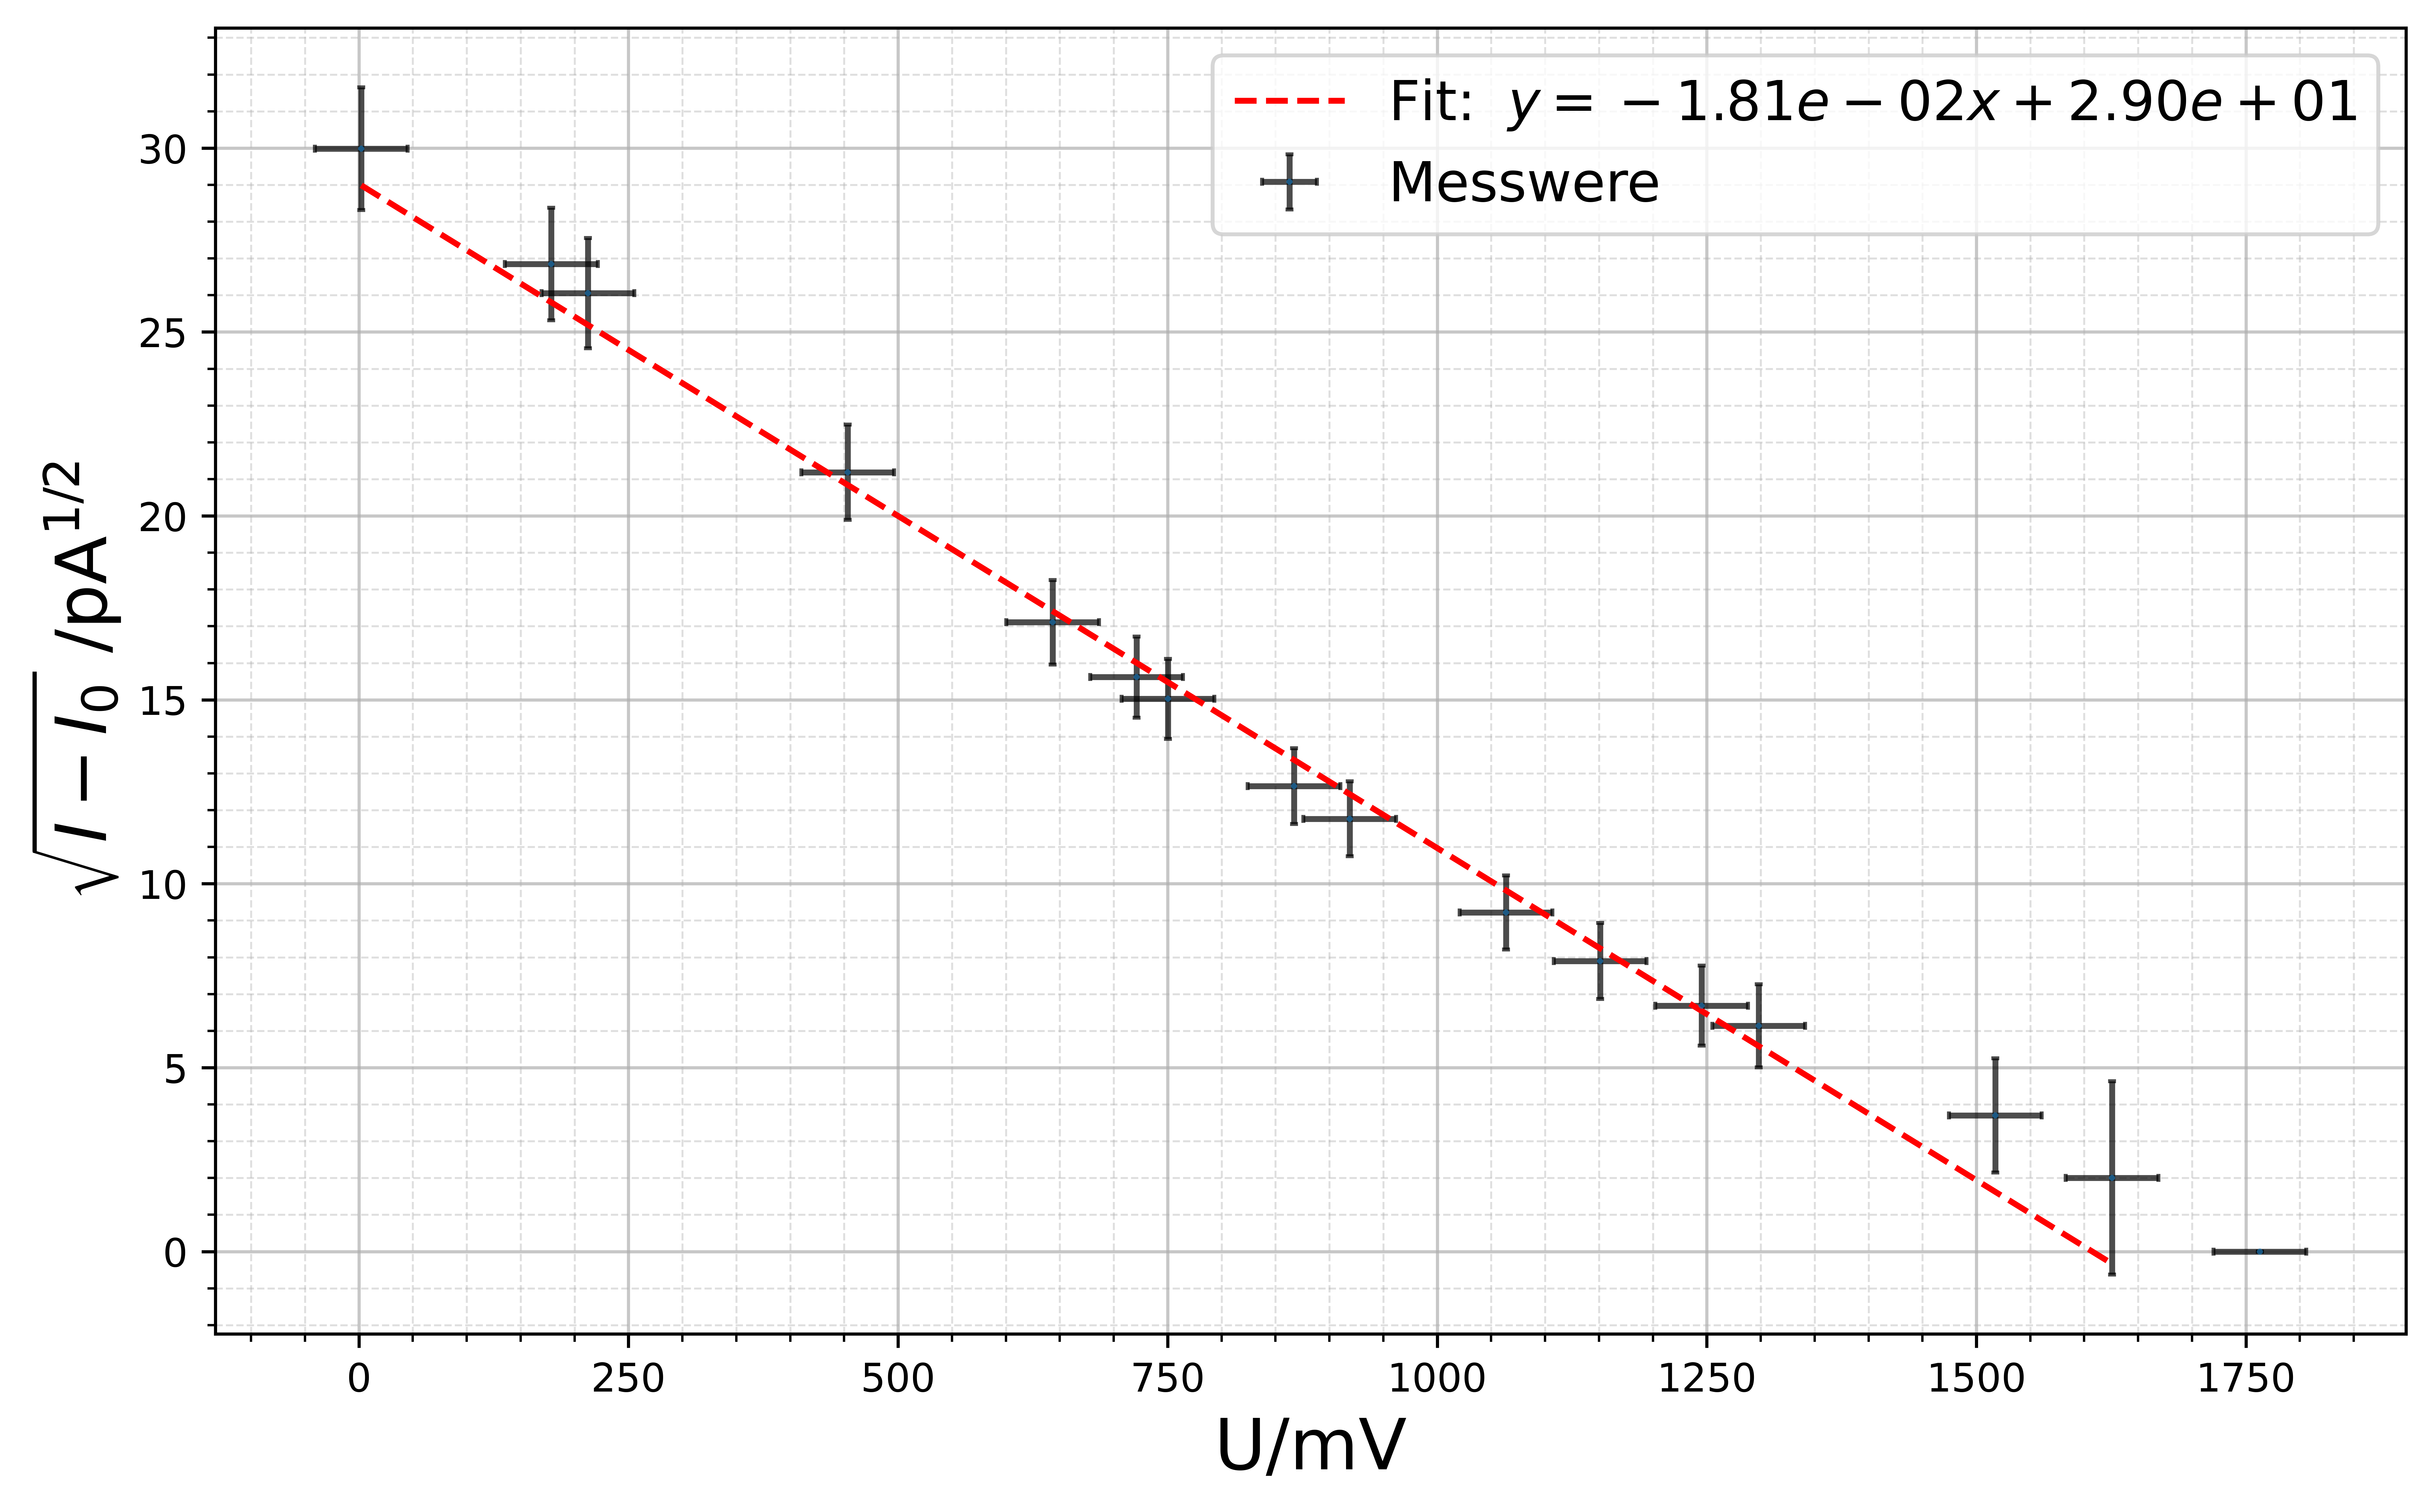
\includegraphics[width=0.95\linewidth]{figs/405_1.png}
    \captionof{figure}{%
      Messung 1 bei $\lambda=\SI{405}{\nm}$. 
      Die Werte und Unsicherheiten sind in \cref{tab:405_first}.%
    }
    \label{fig:405_first}
  \end{minipage}\hfill
  \begin{minipage}[t]{\linewidth}
    \centering
    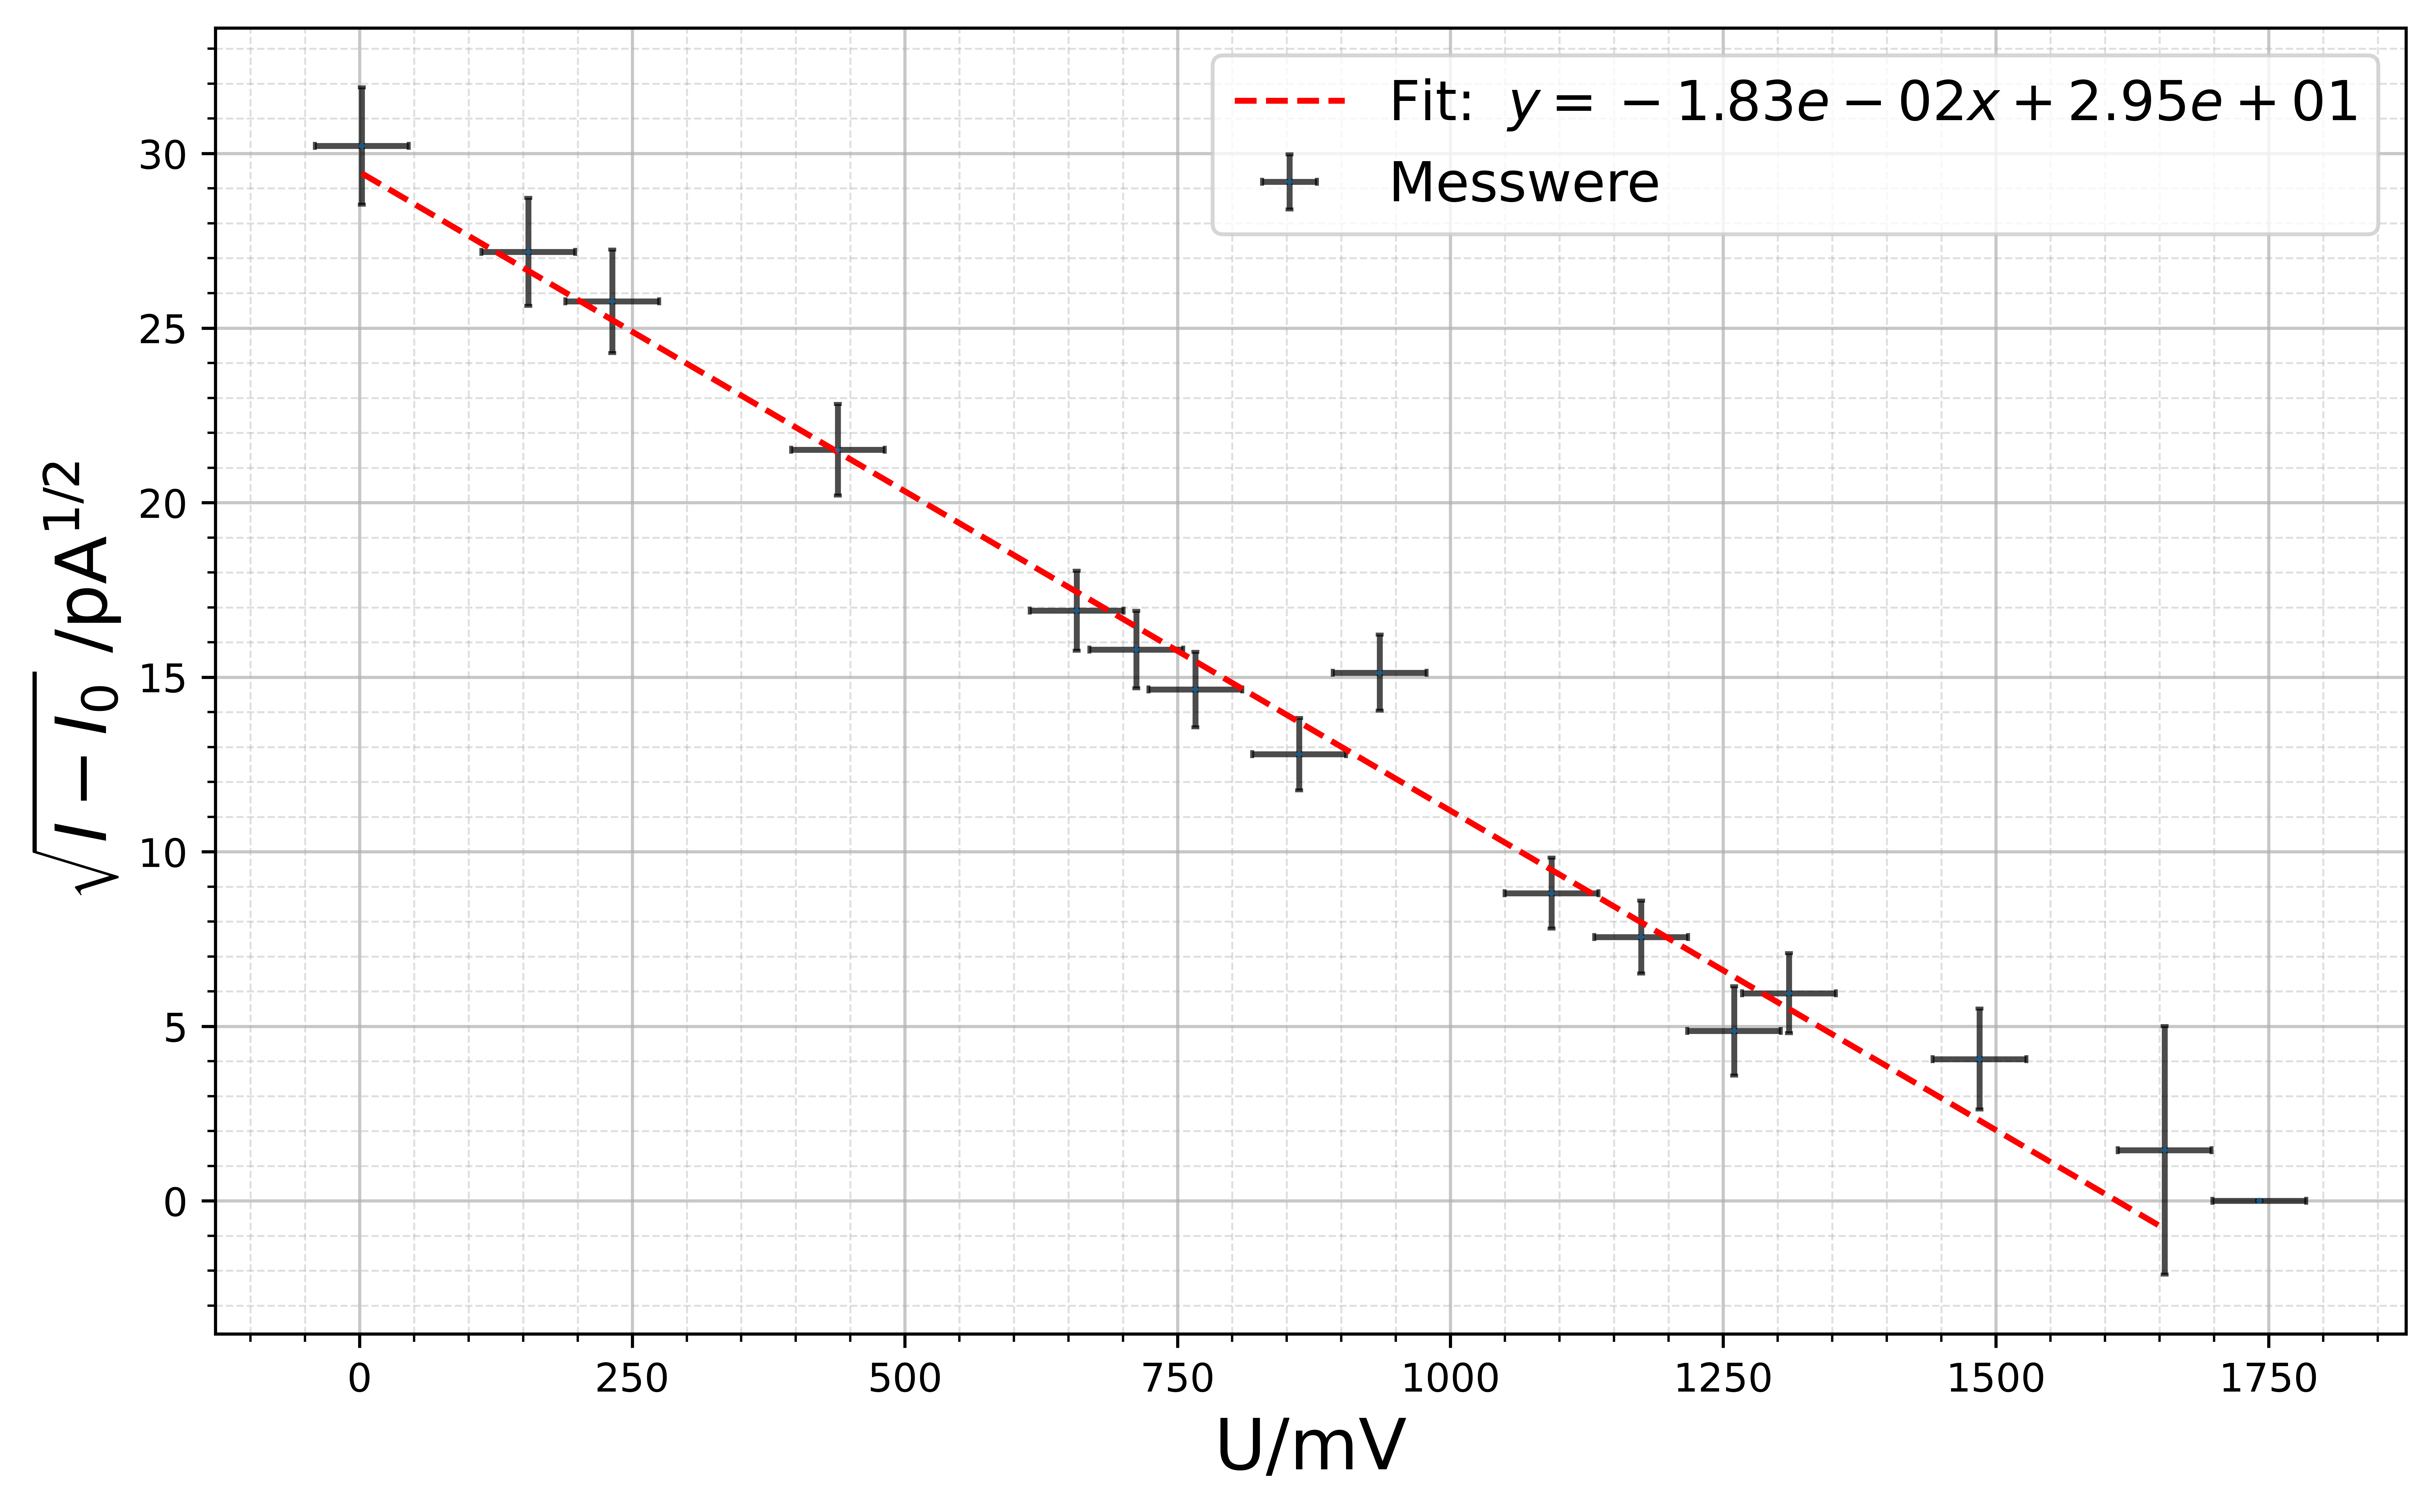
\includegraphics[width=0.95\linewidth]{figs/405_2.png}
    \captionof{figure}{%
      Messung 2 bei $\lambda=\SI{405}{\nm}$. 
      Die Werte und Unsicherheiten sind in \cref{tab:405_second}.%
    }
    \label{fig:405_second}
  \end{minipage}
\end{figure}

\begin{figure}[H]
  \centering
  \begin{minipage}[t]{\linewidth}
    \centering
    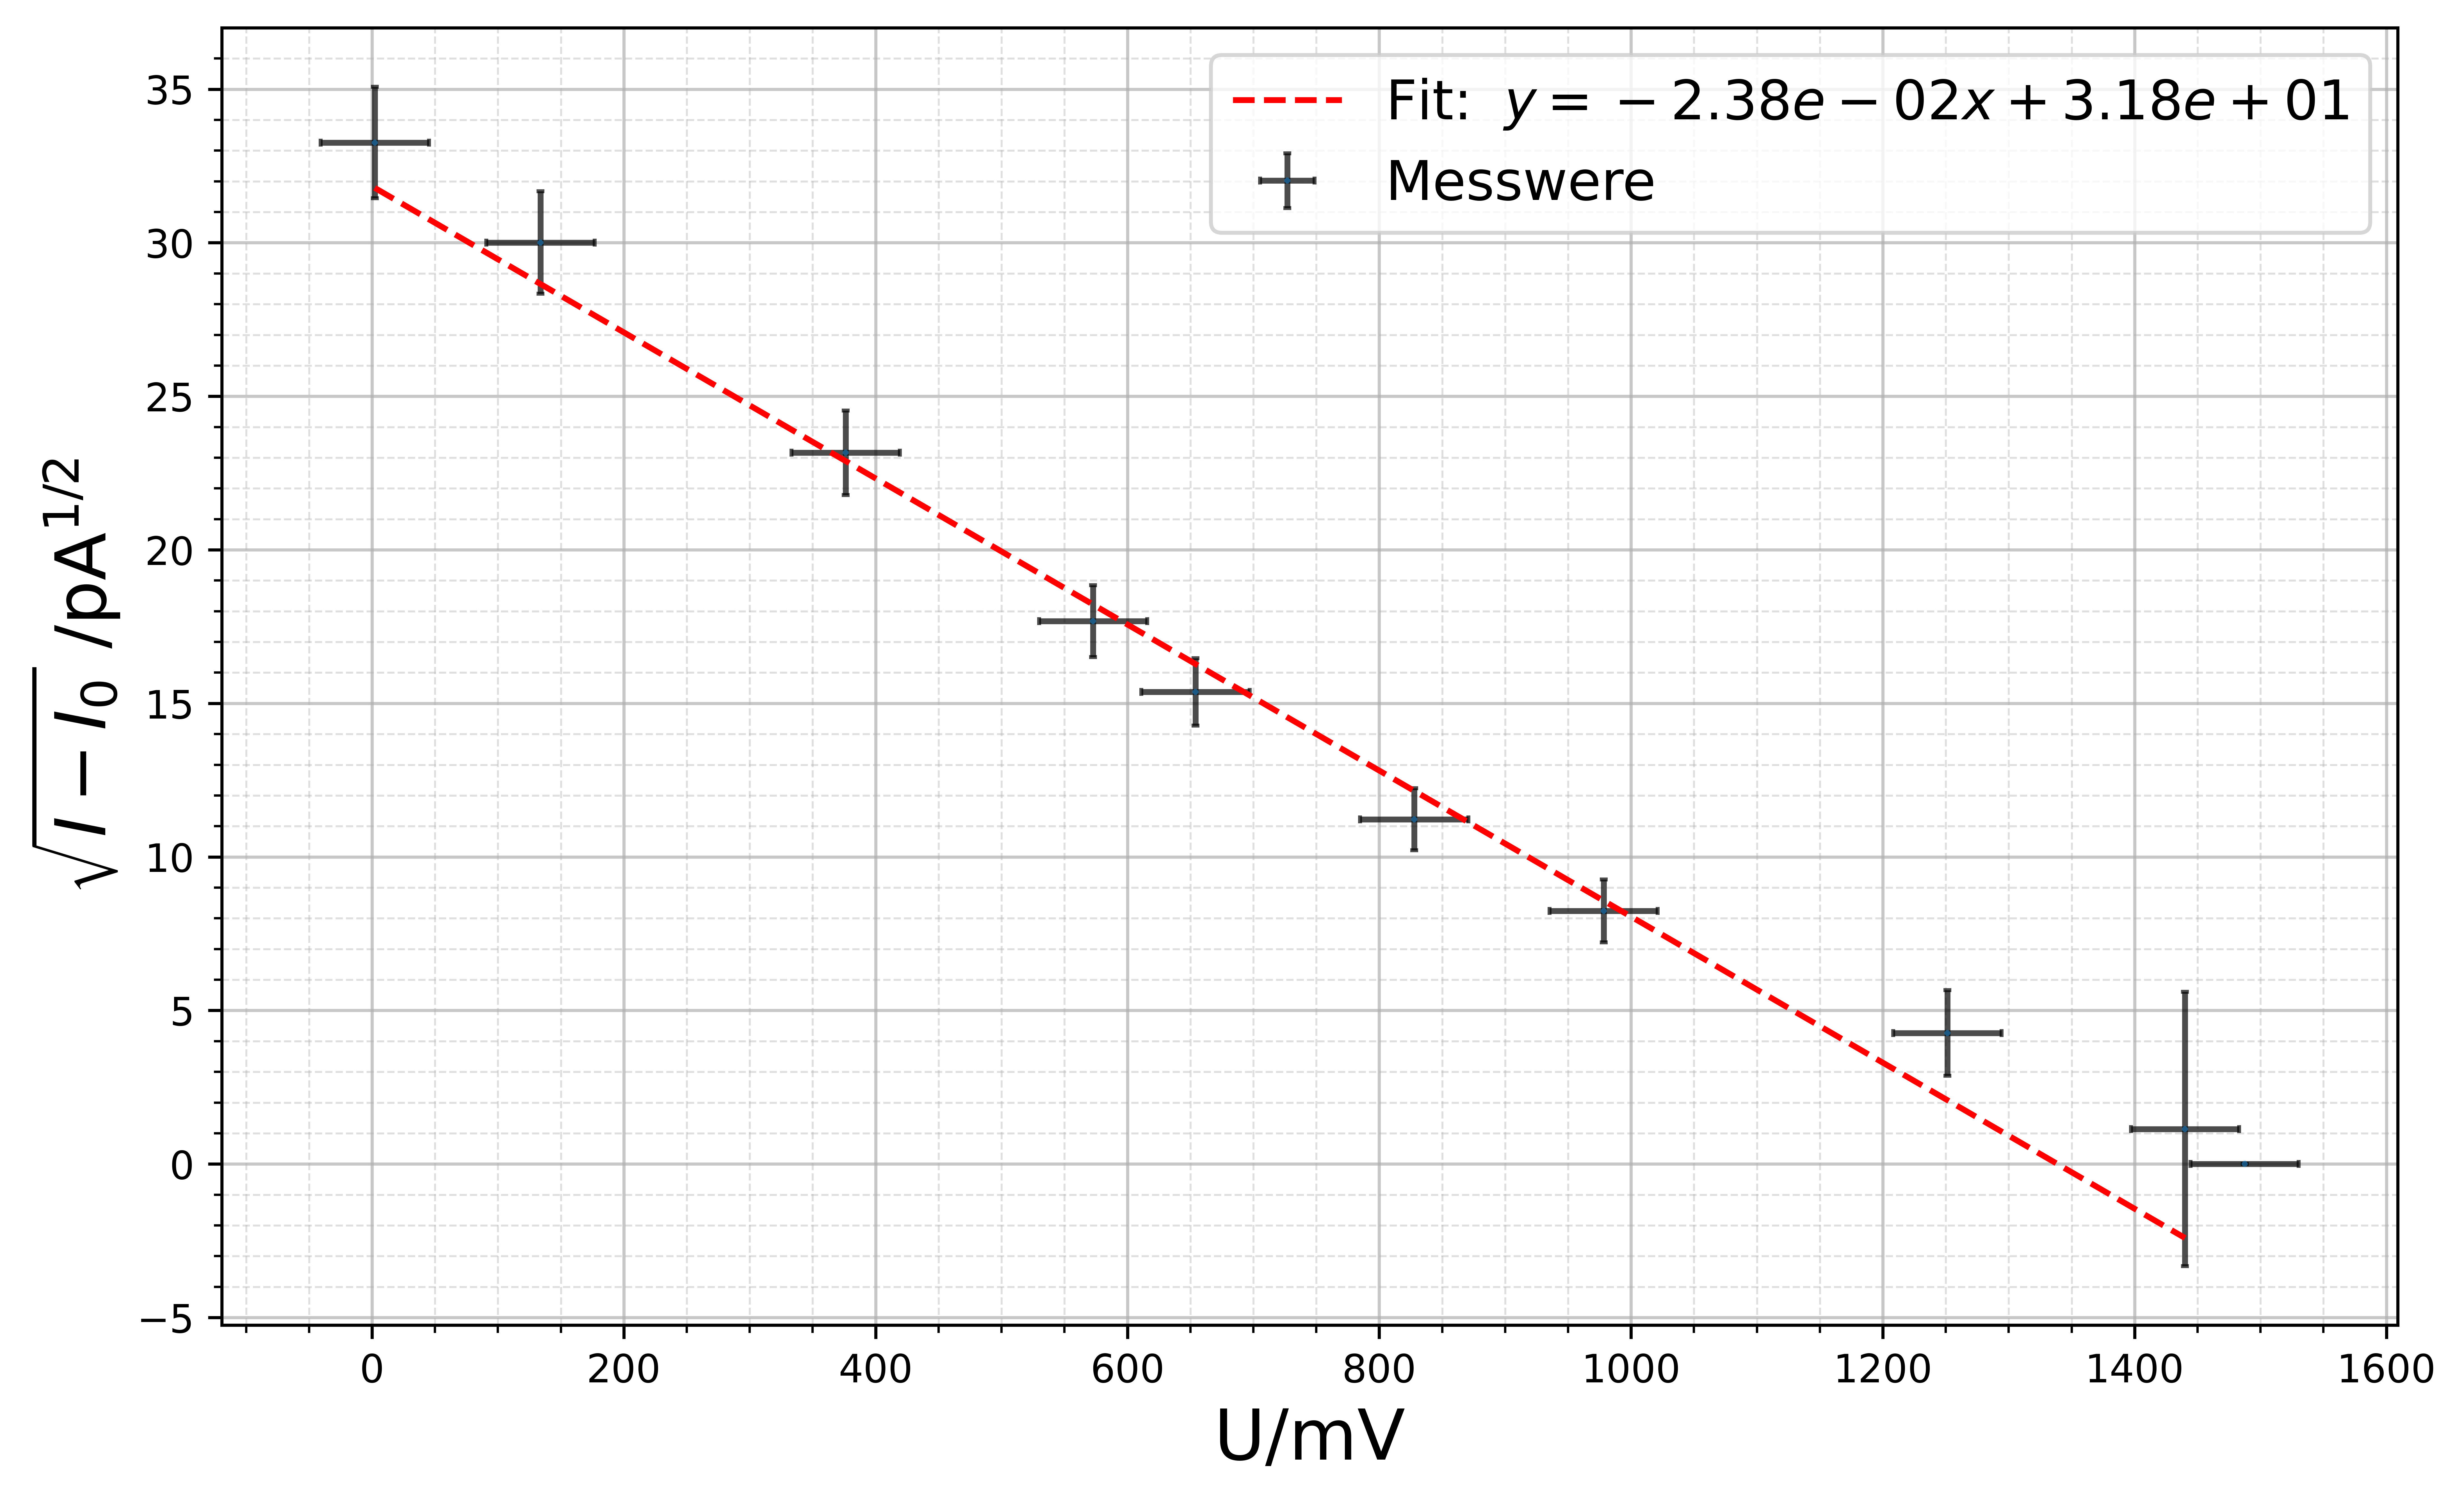
\includegraphics[width=0.95\linewidth]{figs/463_1.png}
    \captionof{figure}{%
      Messung 1 bei $\lambda=\SI{463}{\nm}$. 
      Die Werte und Unsicherheiten sind in \cref{tab:463_first}.%
    }
    \label{fig:463_first}
  \end{minipage}\hfill
  \begin{minipage}[t]{\linewidth}
    \centering
    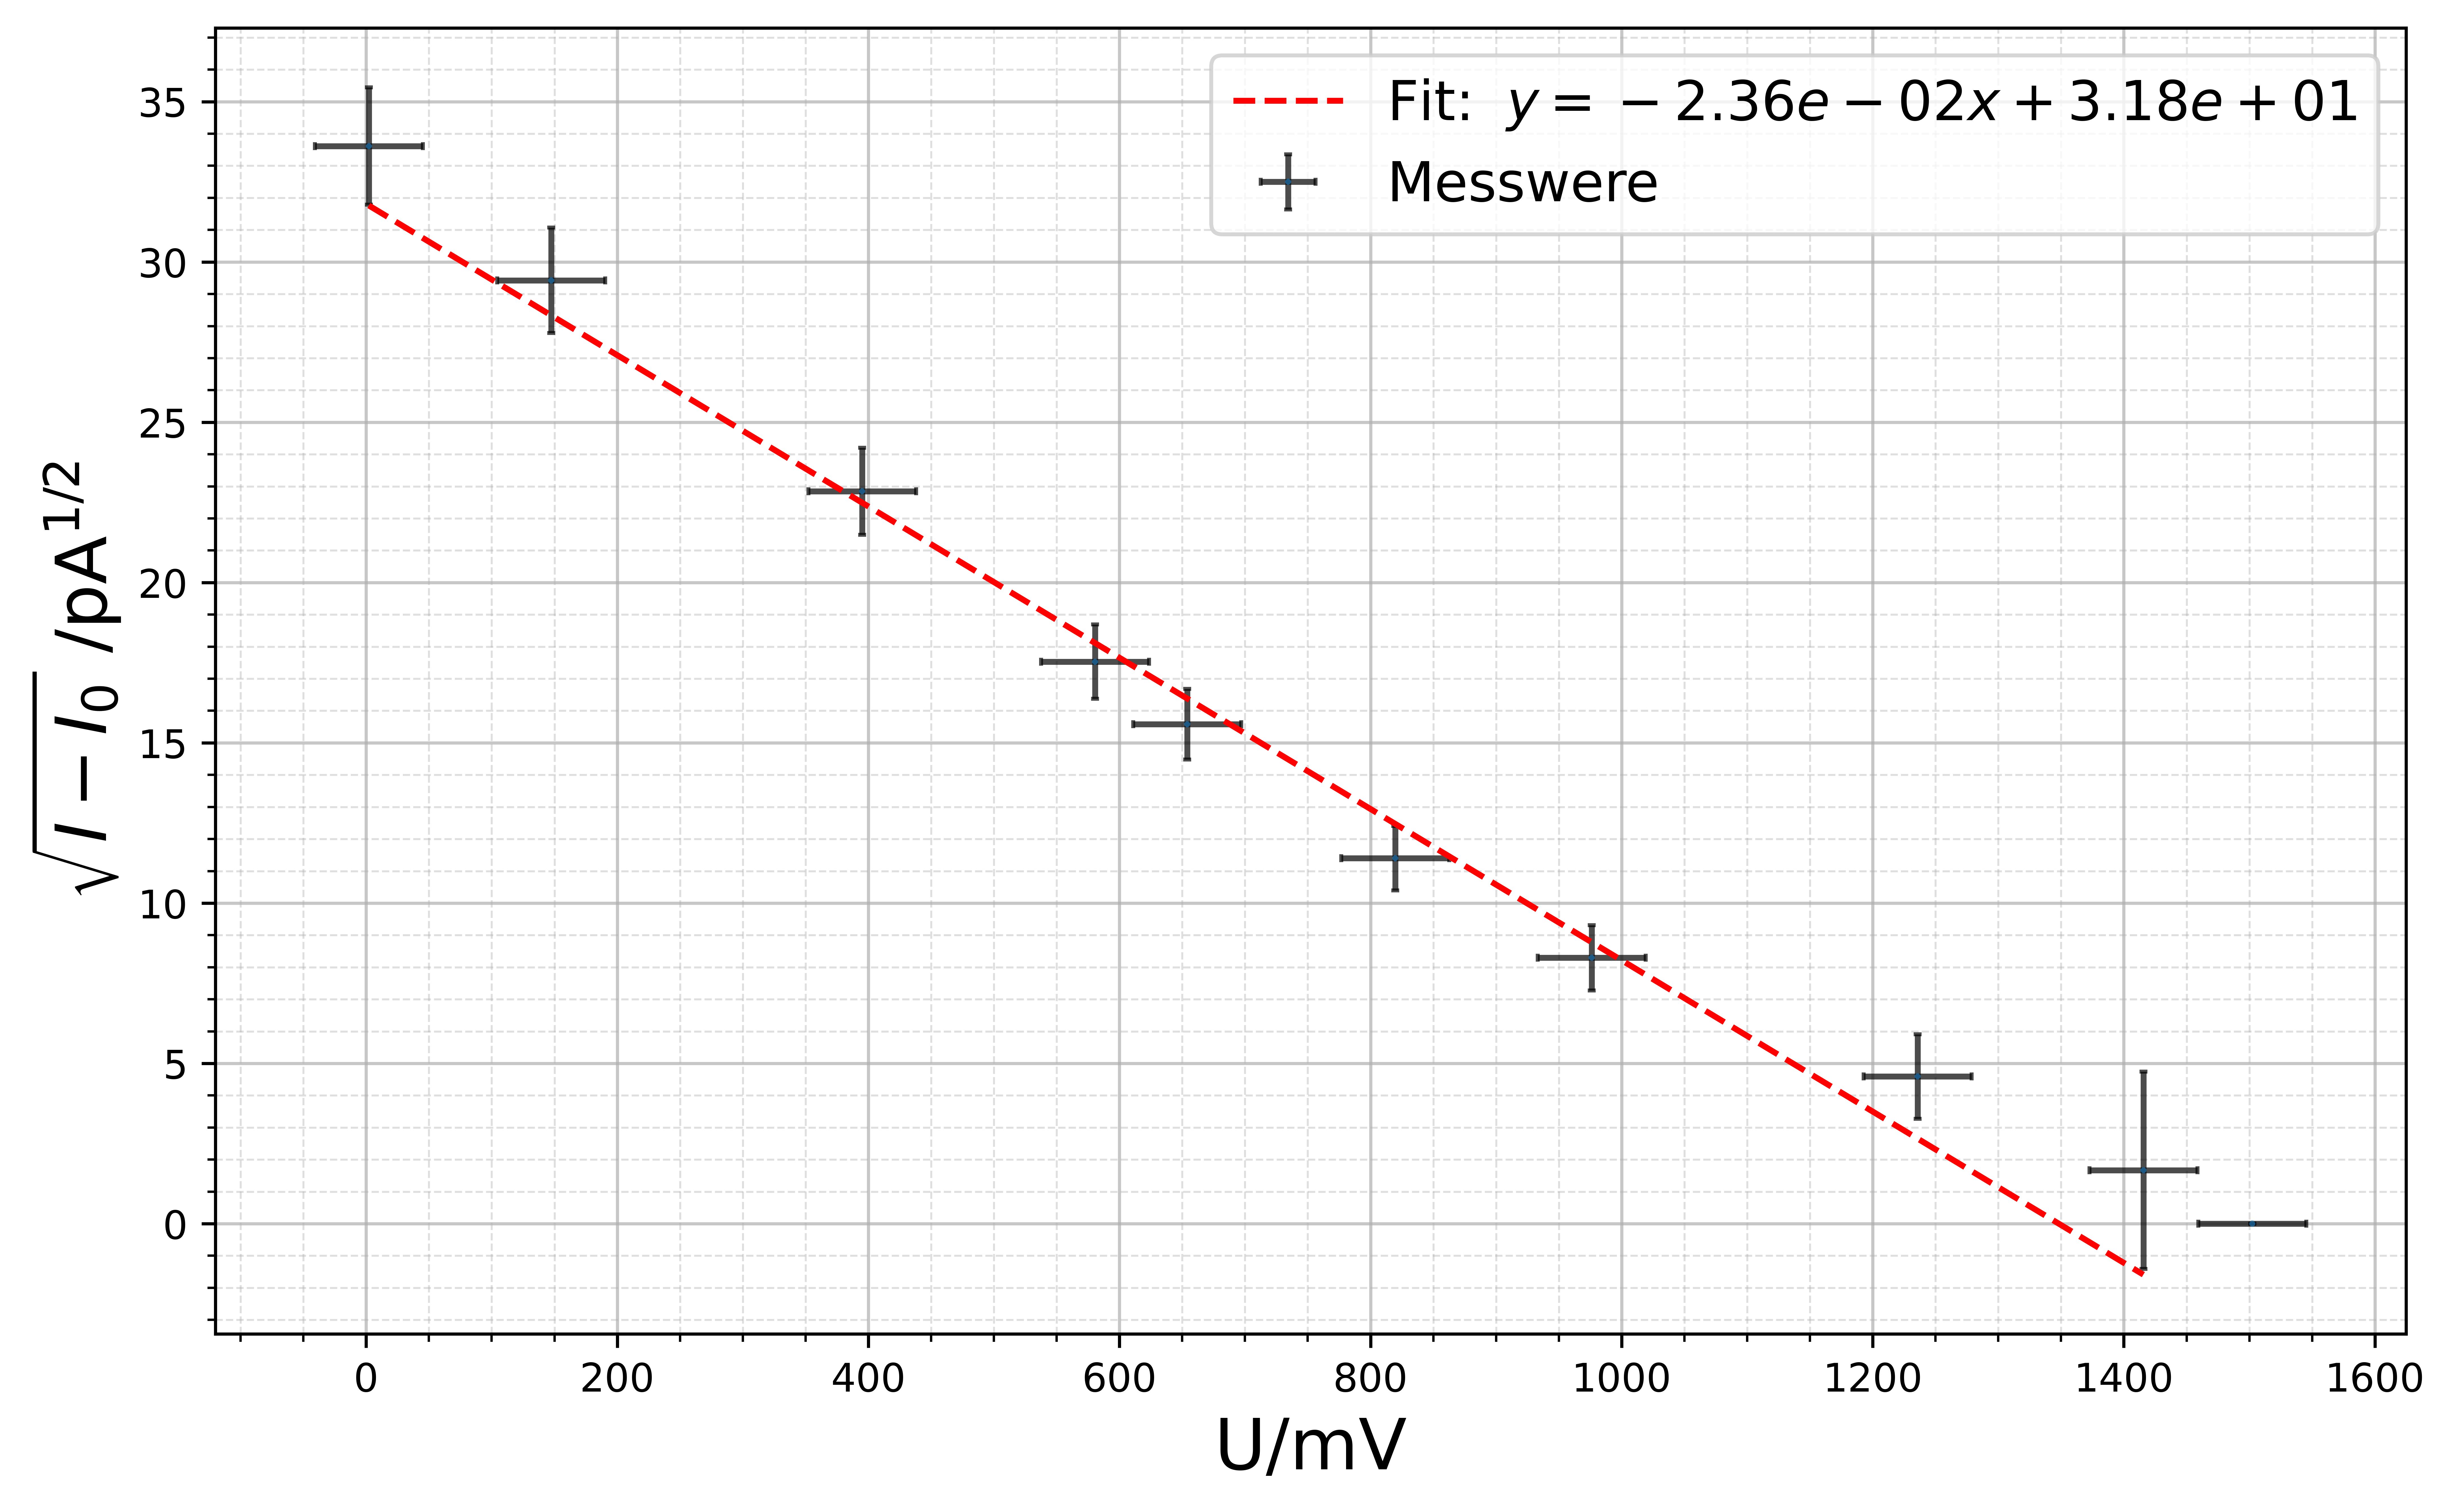
\includegraphics[width=0.95\linewidth]{figs/463_2.png}
    \captionof{figure}{%
      Messung 2 bei $\lambda=\SI{463}{\nm}$. 
      Die Werte und Unsicherheiten sind in \cref{tab:463_second}.%
    }
    \label{fig:463_second}
  \end{minipage}
\end{figure}


\begin{figure}[H]
  \centering
  \begin{minipage}[t]{\linewidth}
    \centering
    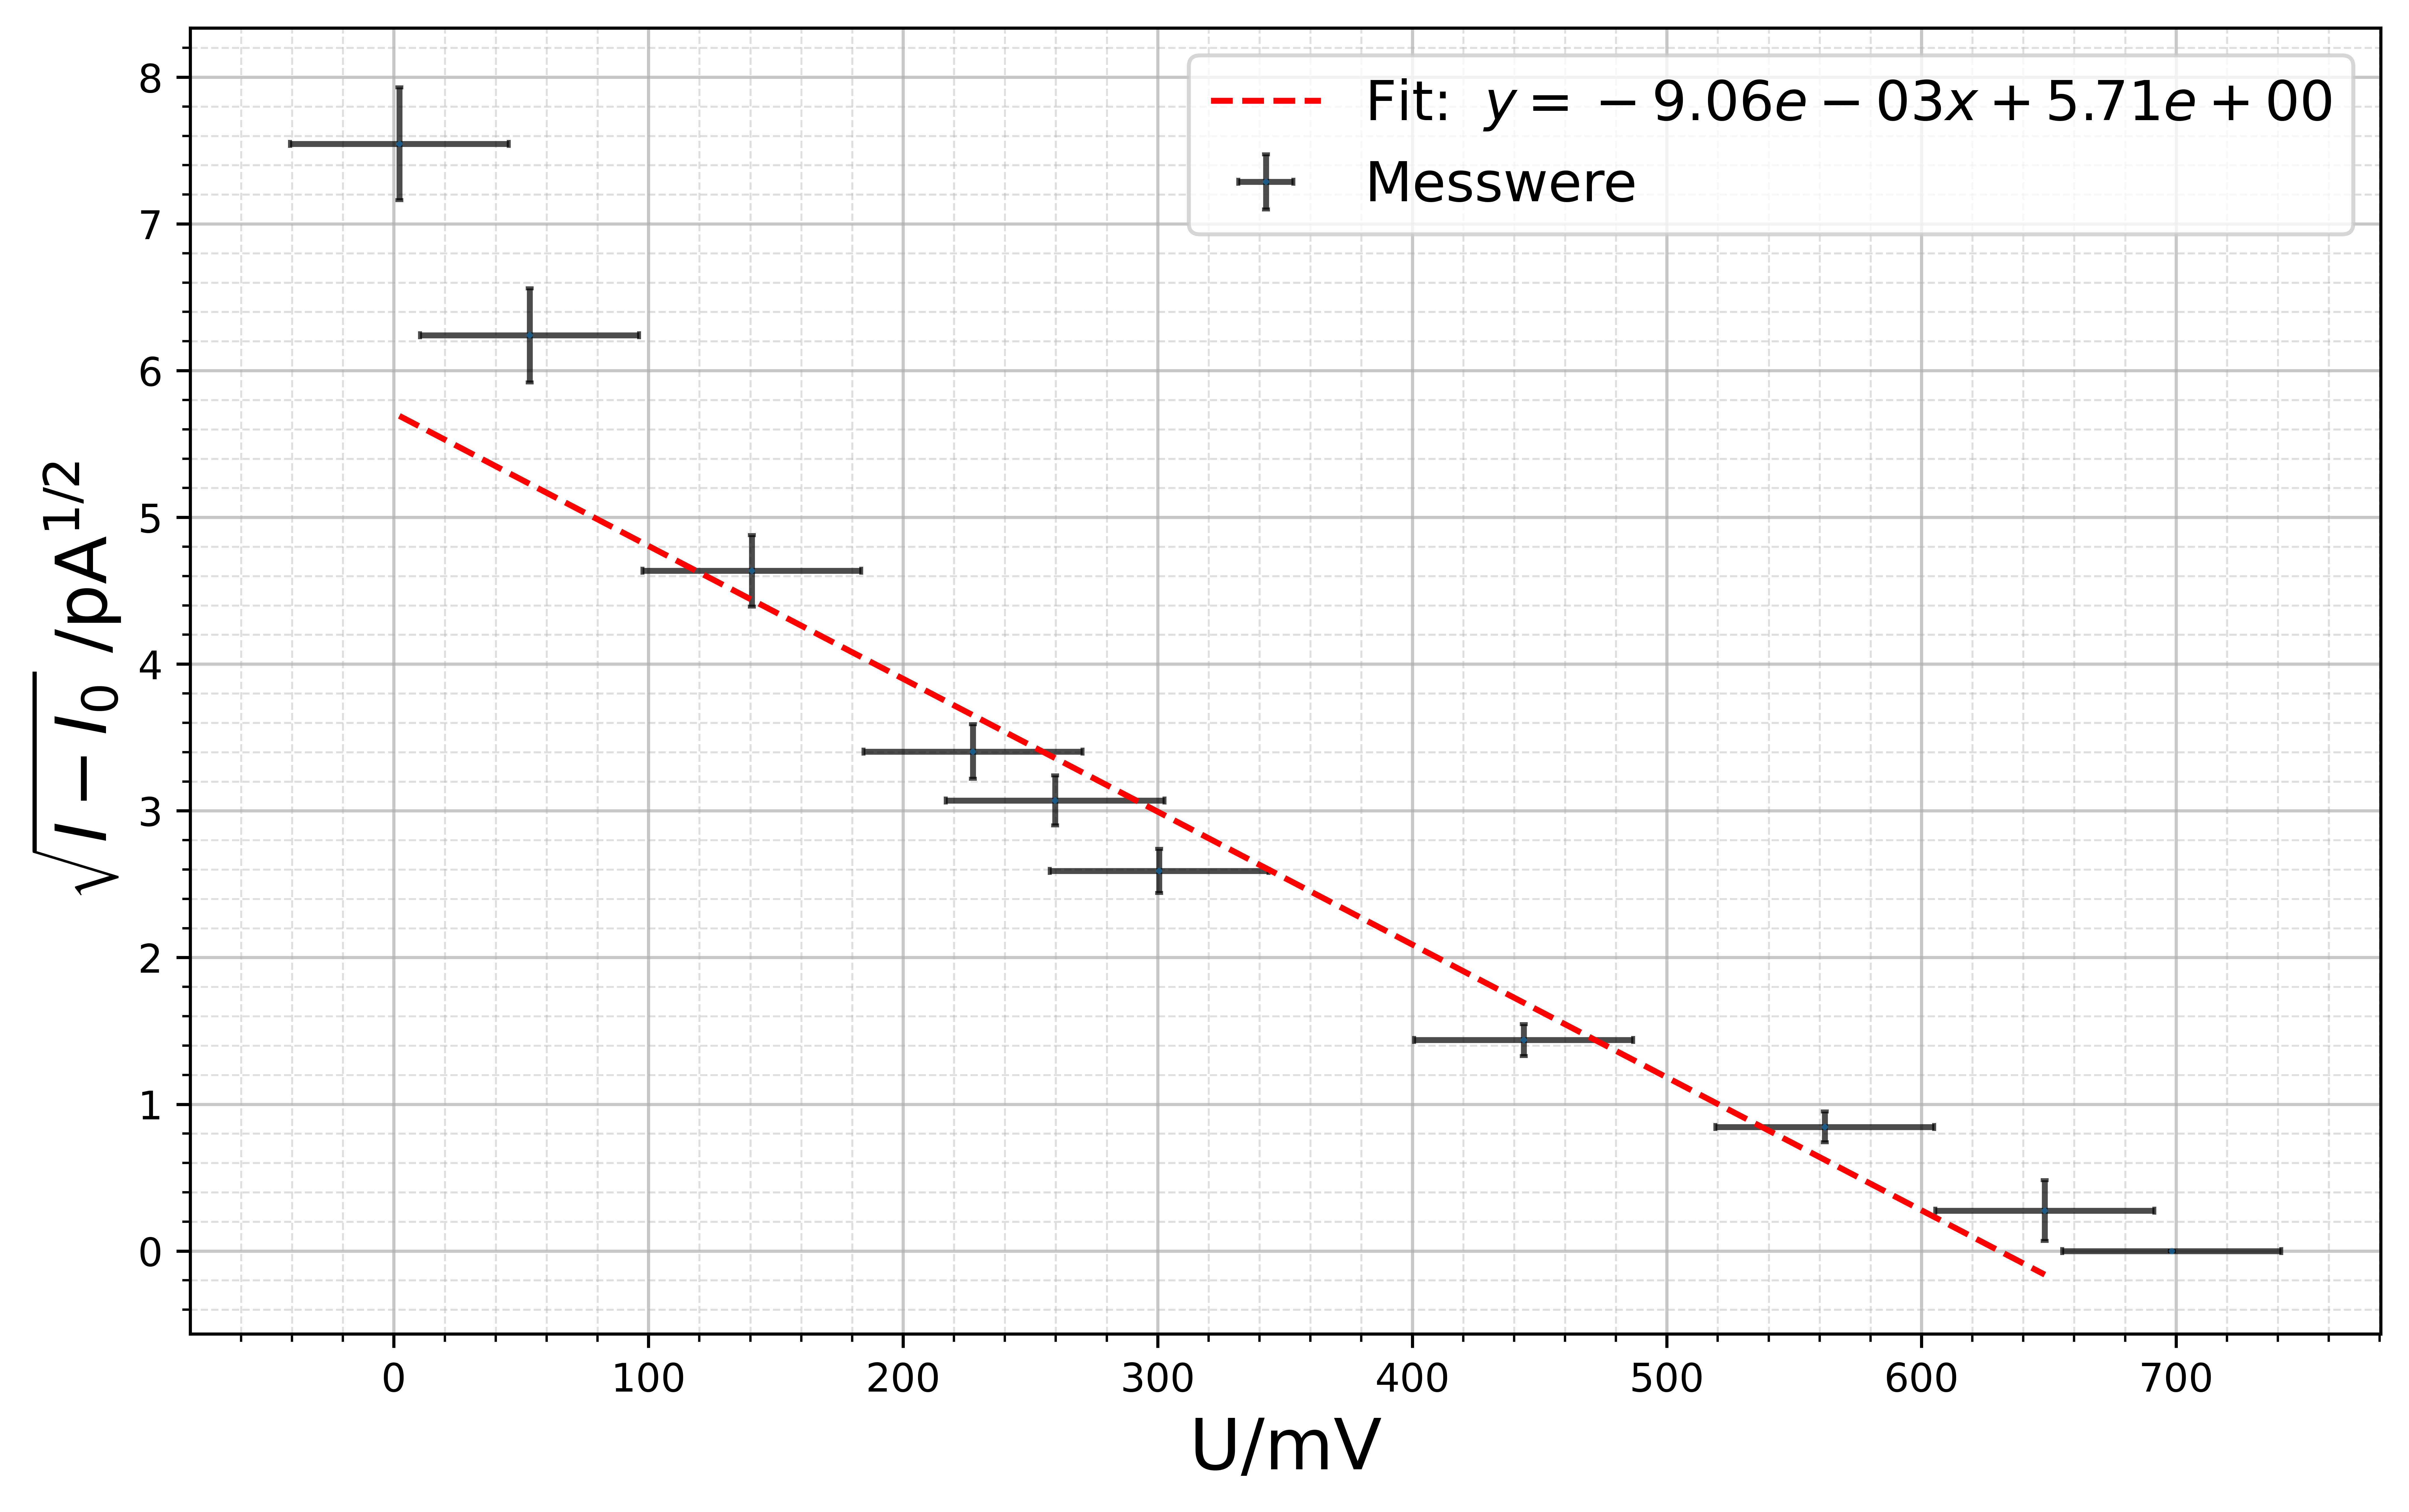
\includegraphics[width=0.95\linewidth]{figs/546_1.png}
    \captionof{figure}{%
      Messung 1 bei $\lambda=\SI{546}{\nm}$. 
      Die Werte und Unsicherheiten sind in \cref{tab:546_first}.%
    }
    \label{fig:546_first}
  \end{minipage}\hfill
  \begin{minipage}[t]{\linewidth}
    \centering
    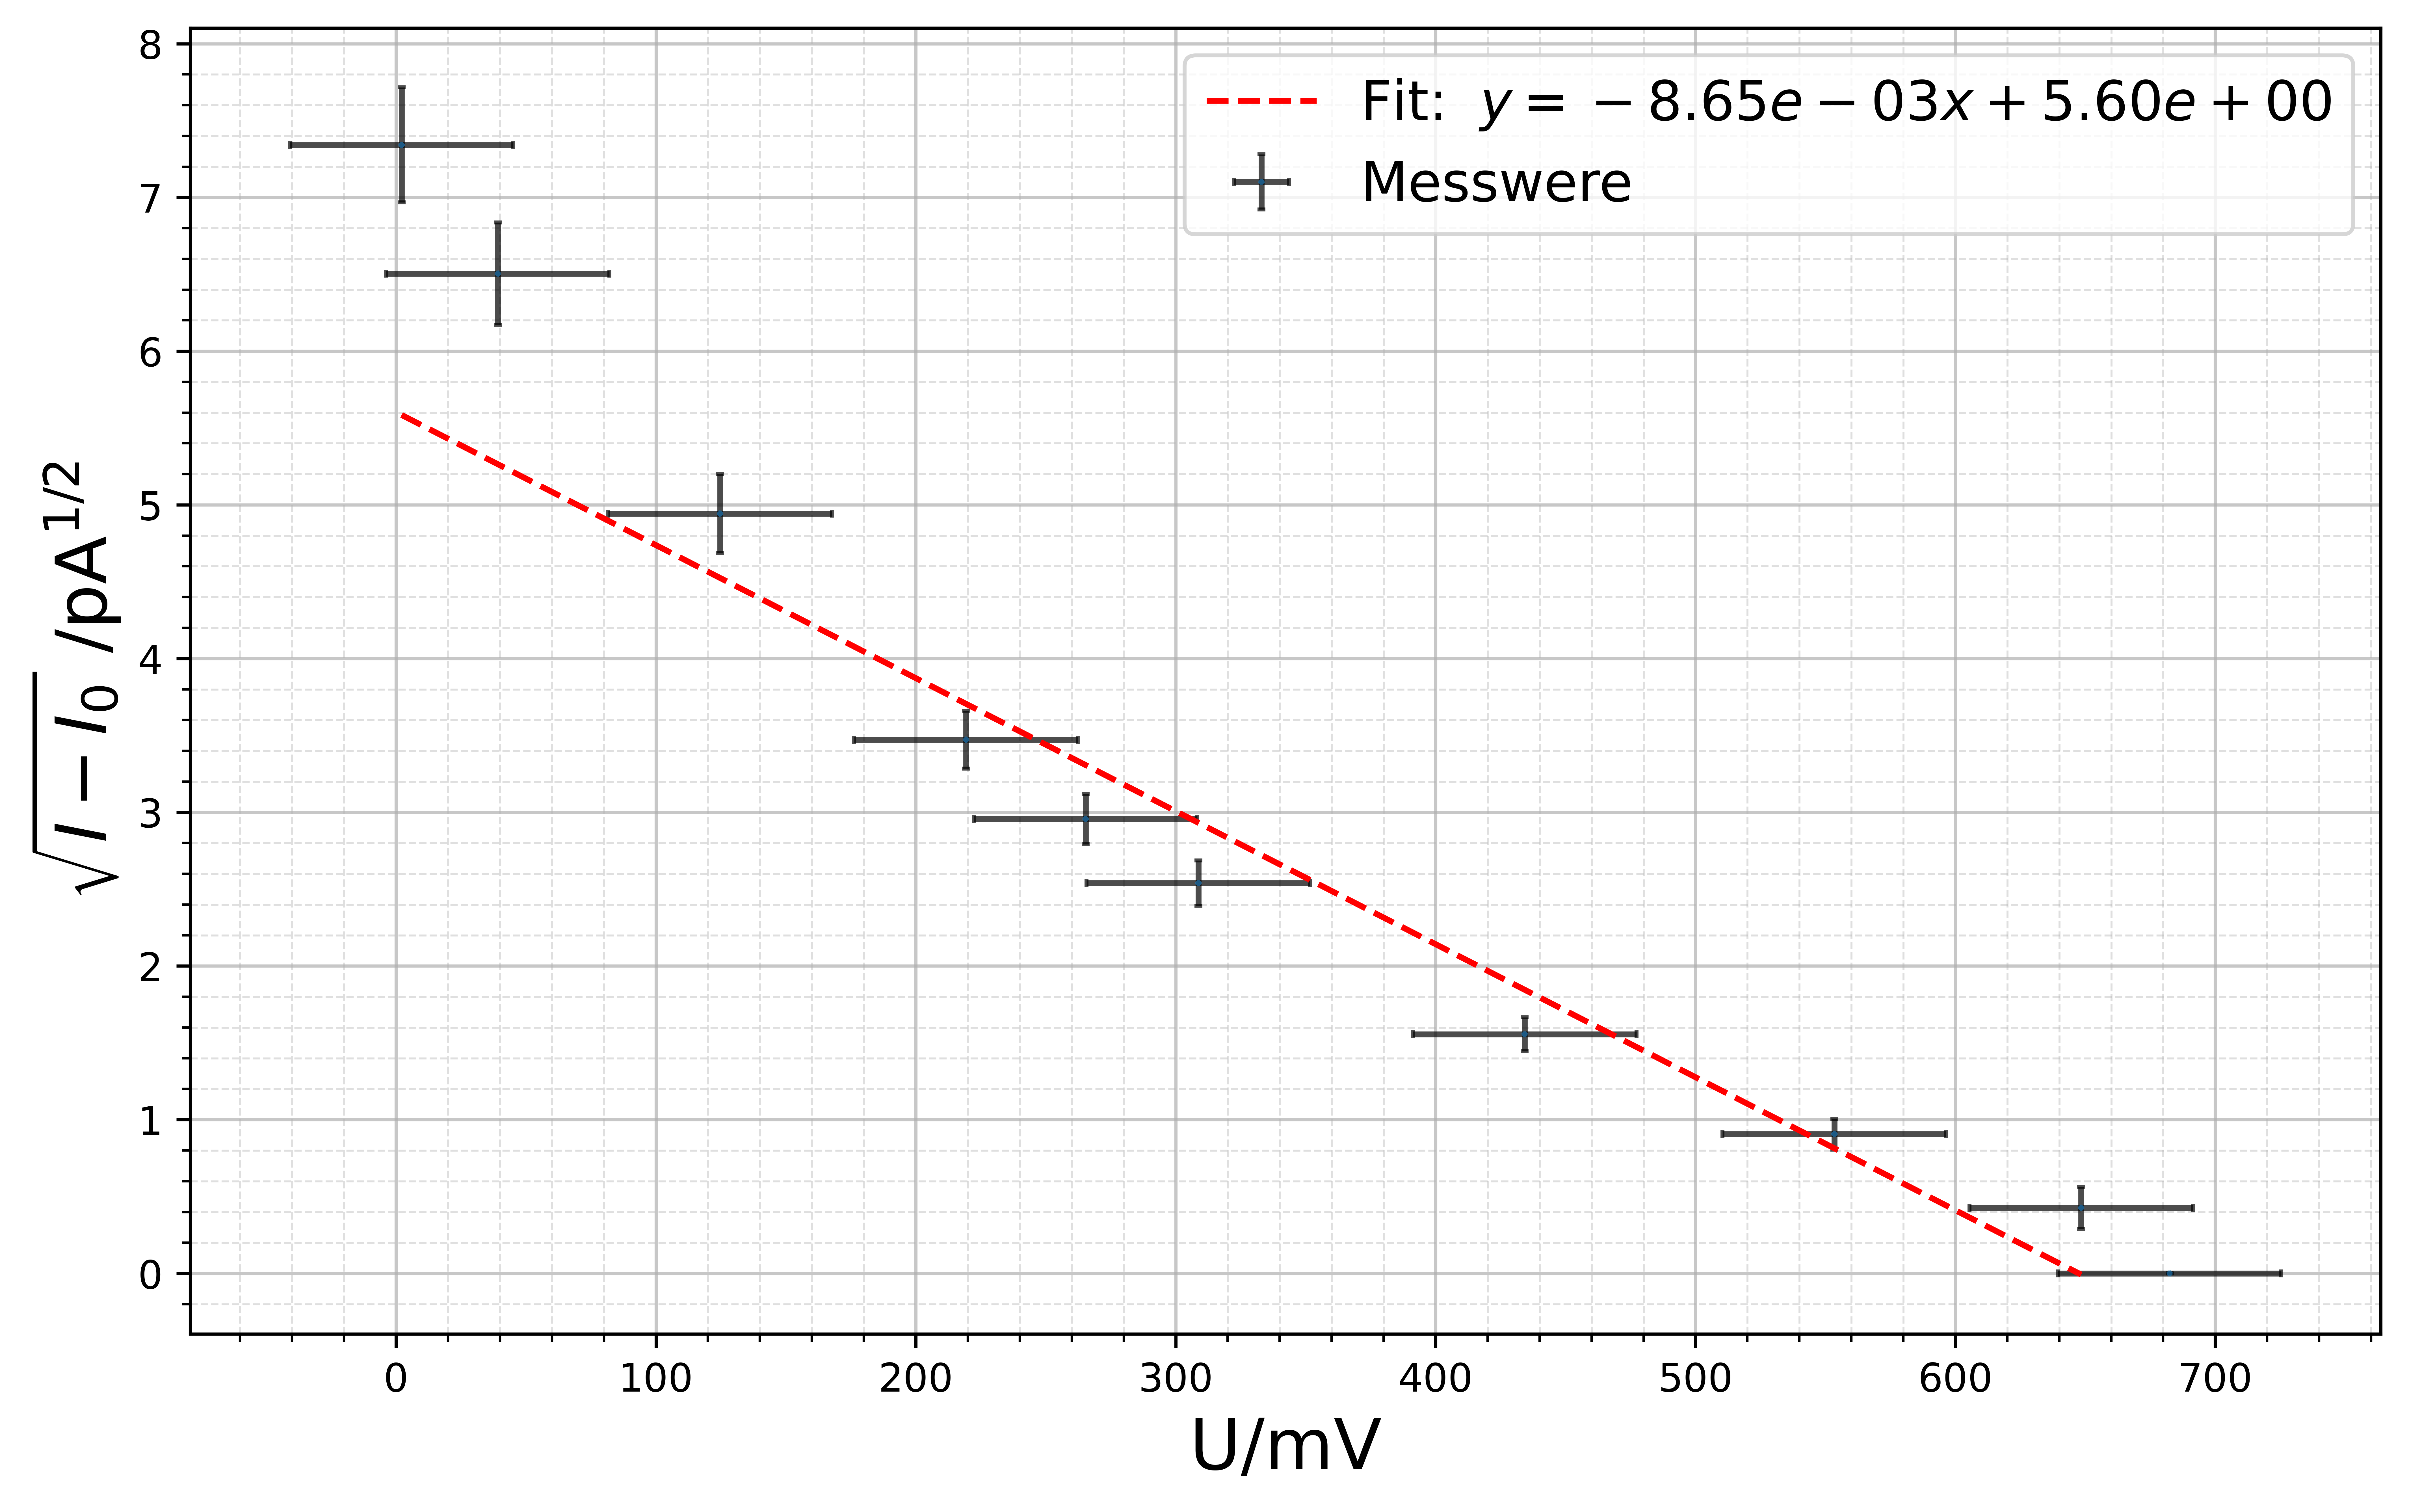
\includegraphics[width=0.95\linewidth]{figs/546_2.png}
    \captionof{figure}{%
      Messung 2 bei $\lambda=\SI{546}{\nm}$. 
      Die Werte und Unsicherheiten sind in \cref{tab:546_second}.%
    }
    \label{fig:546_second}
  \end{minipage}
\end{figure}

\begin{figure}[H]
  \centering
  \begin{minipage}[t]{\linewidth}
    \centering
    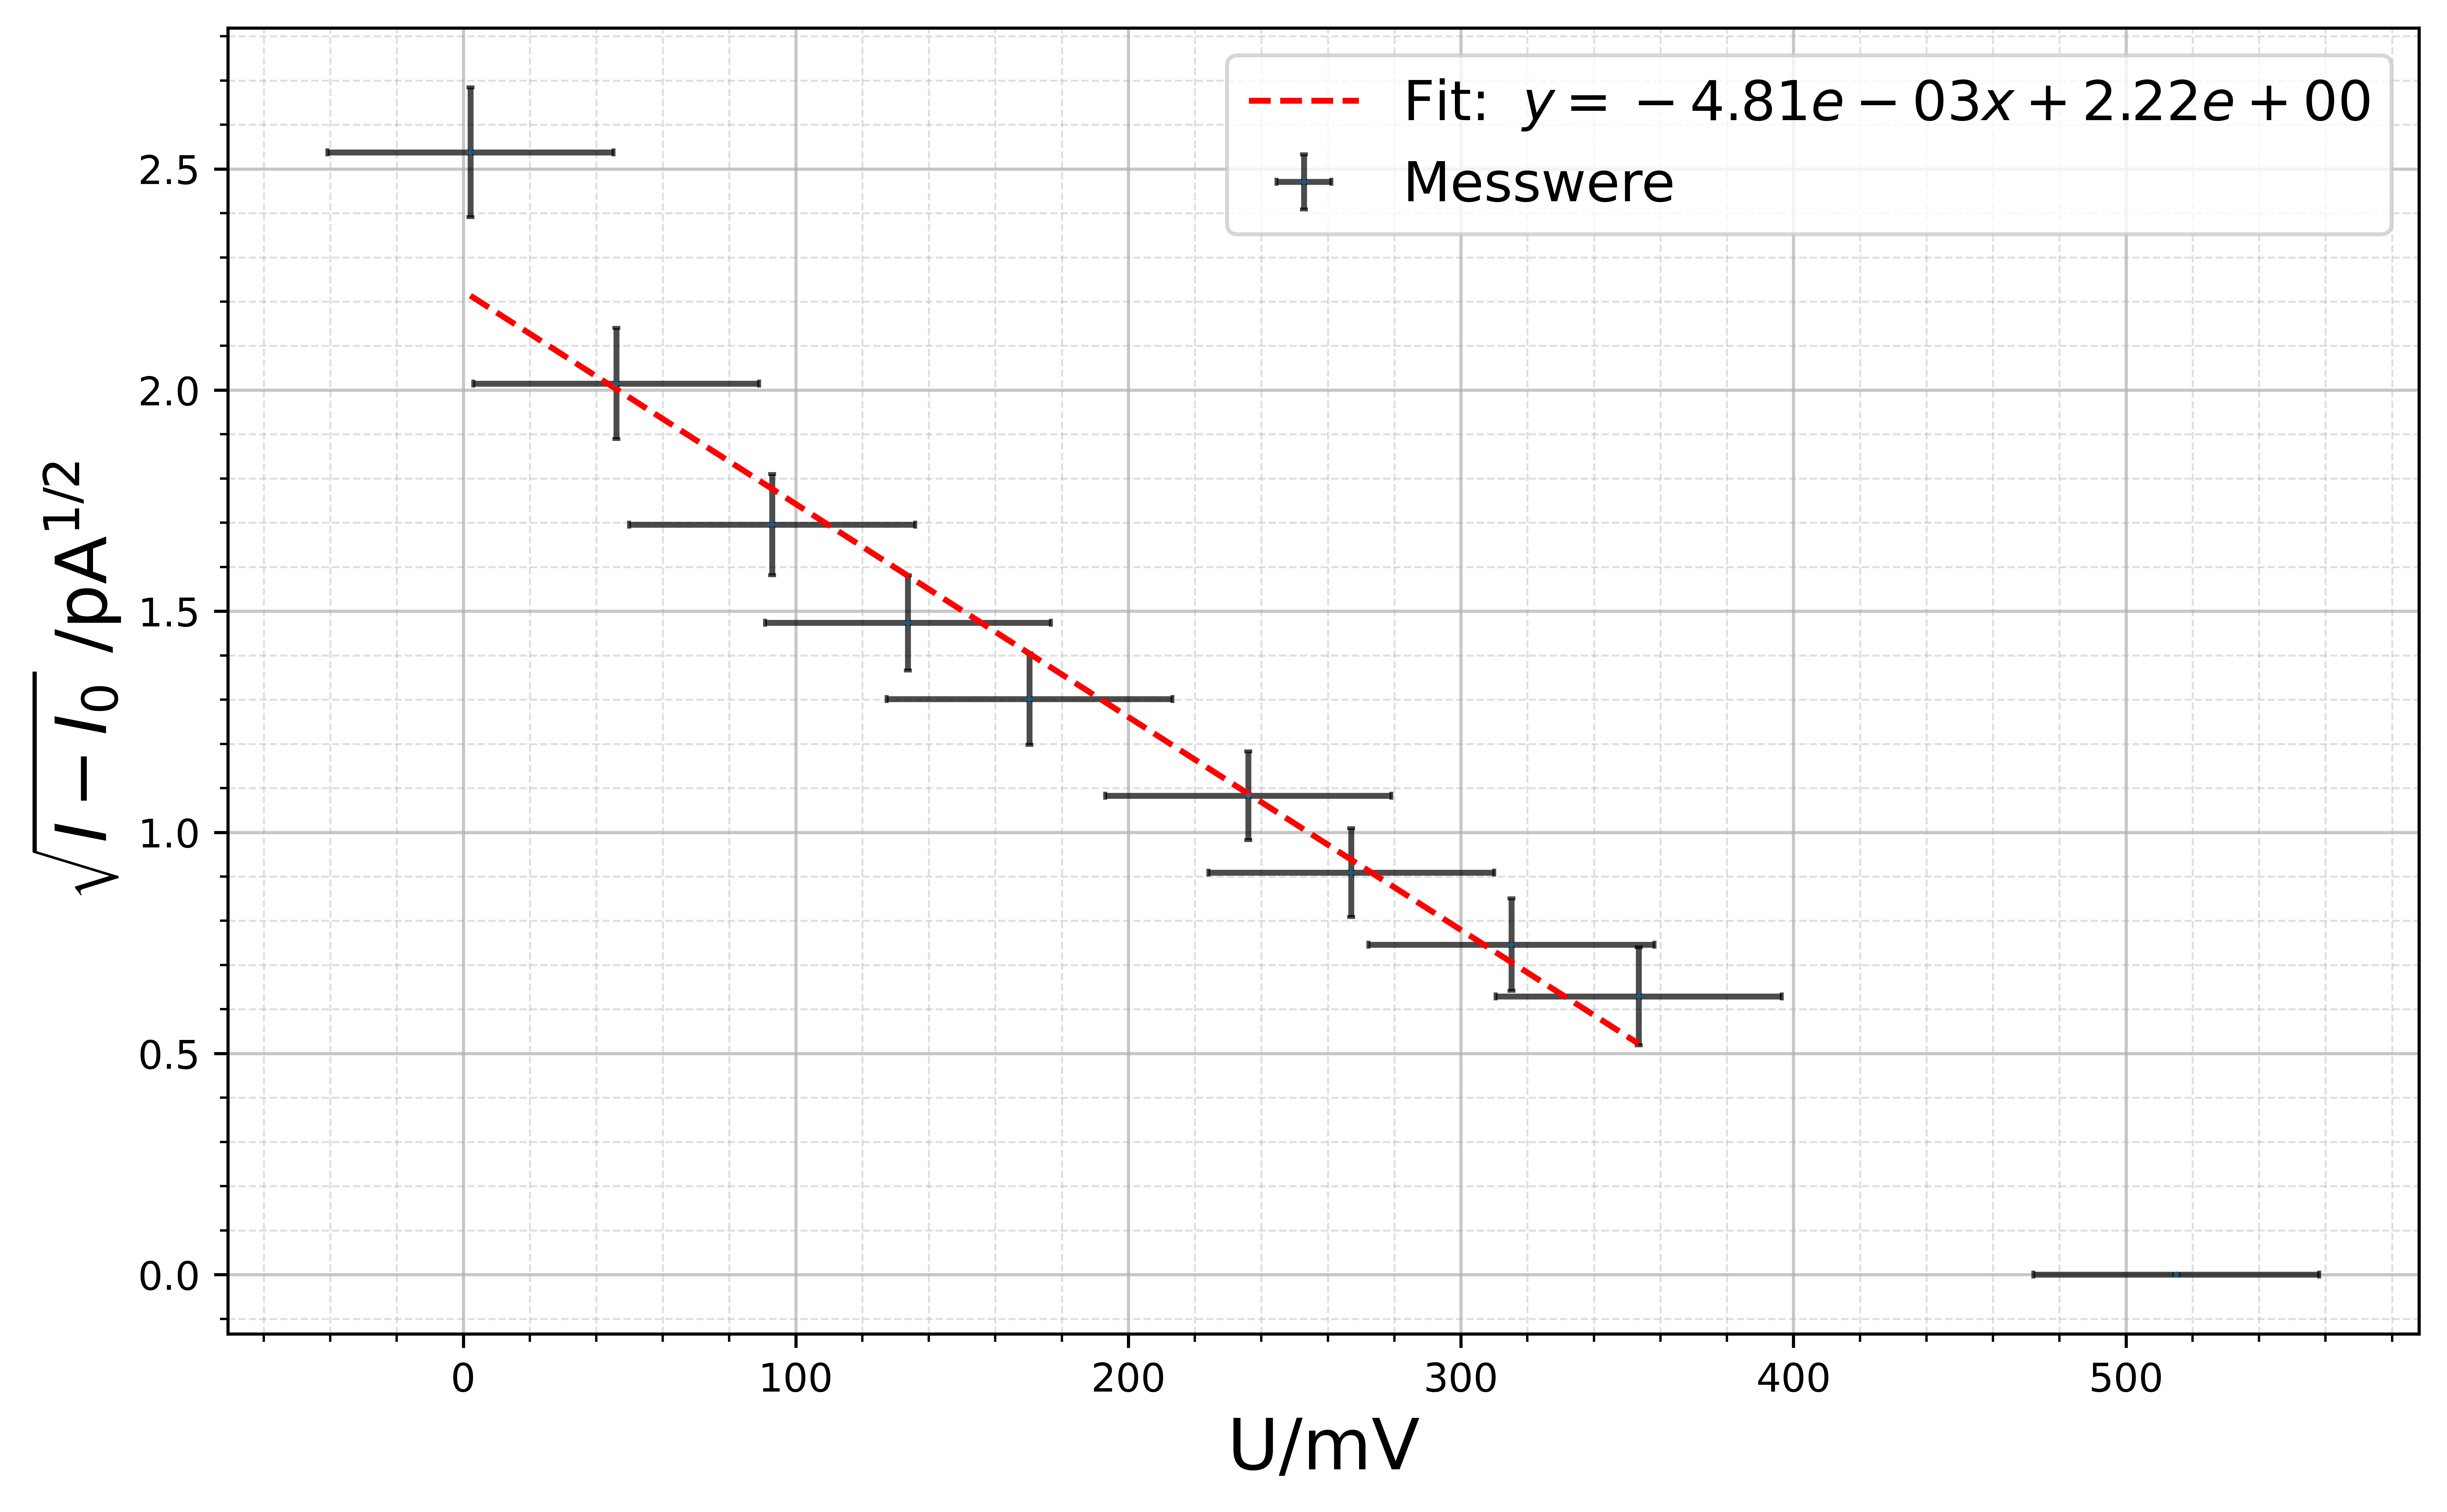
\includegraphics[width=0.95\linewidth]{figs/578_1.png}
    \captionof{figure}{%
      Messung 1 bei $\lambda=\SI{578}{\nm}$. 
      Die Werte und Unsicherheiten sind in \cref{tab:578_first}.%
    }
    \label{fig:578_first}
  \end{minipage}\hfill
  \begin{minipage}[t]{\linewidth}
    \centering
    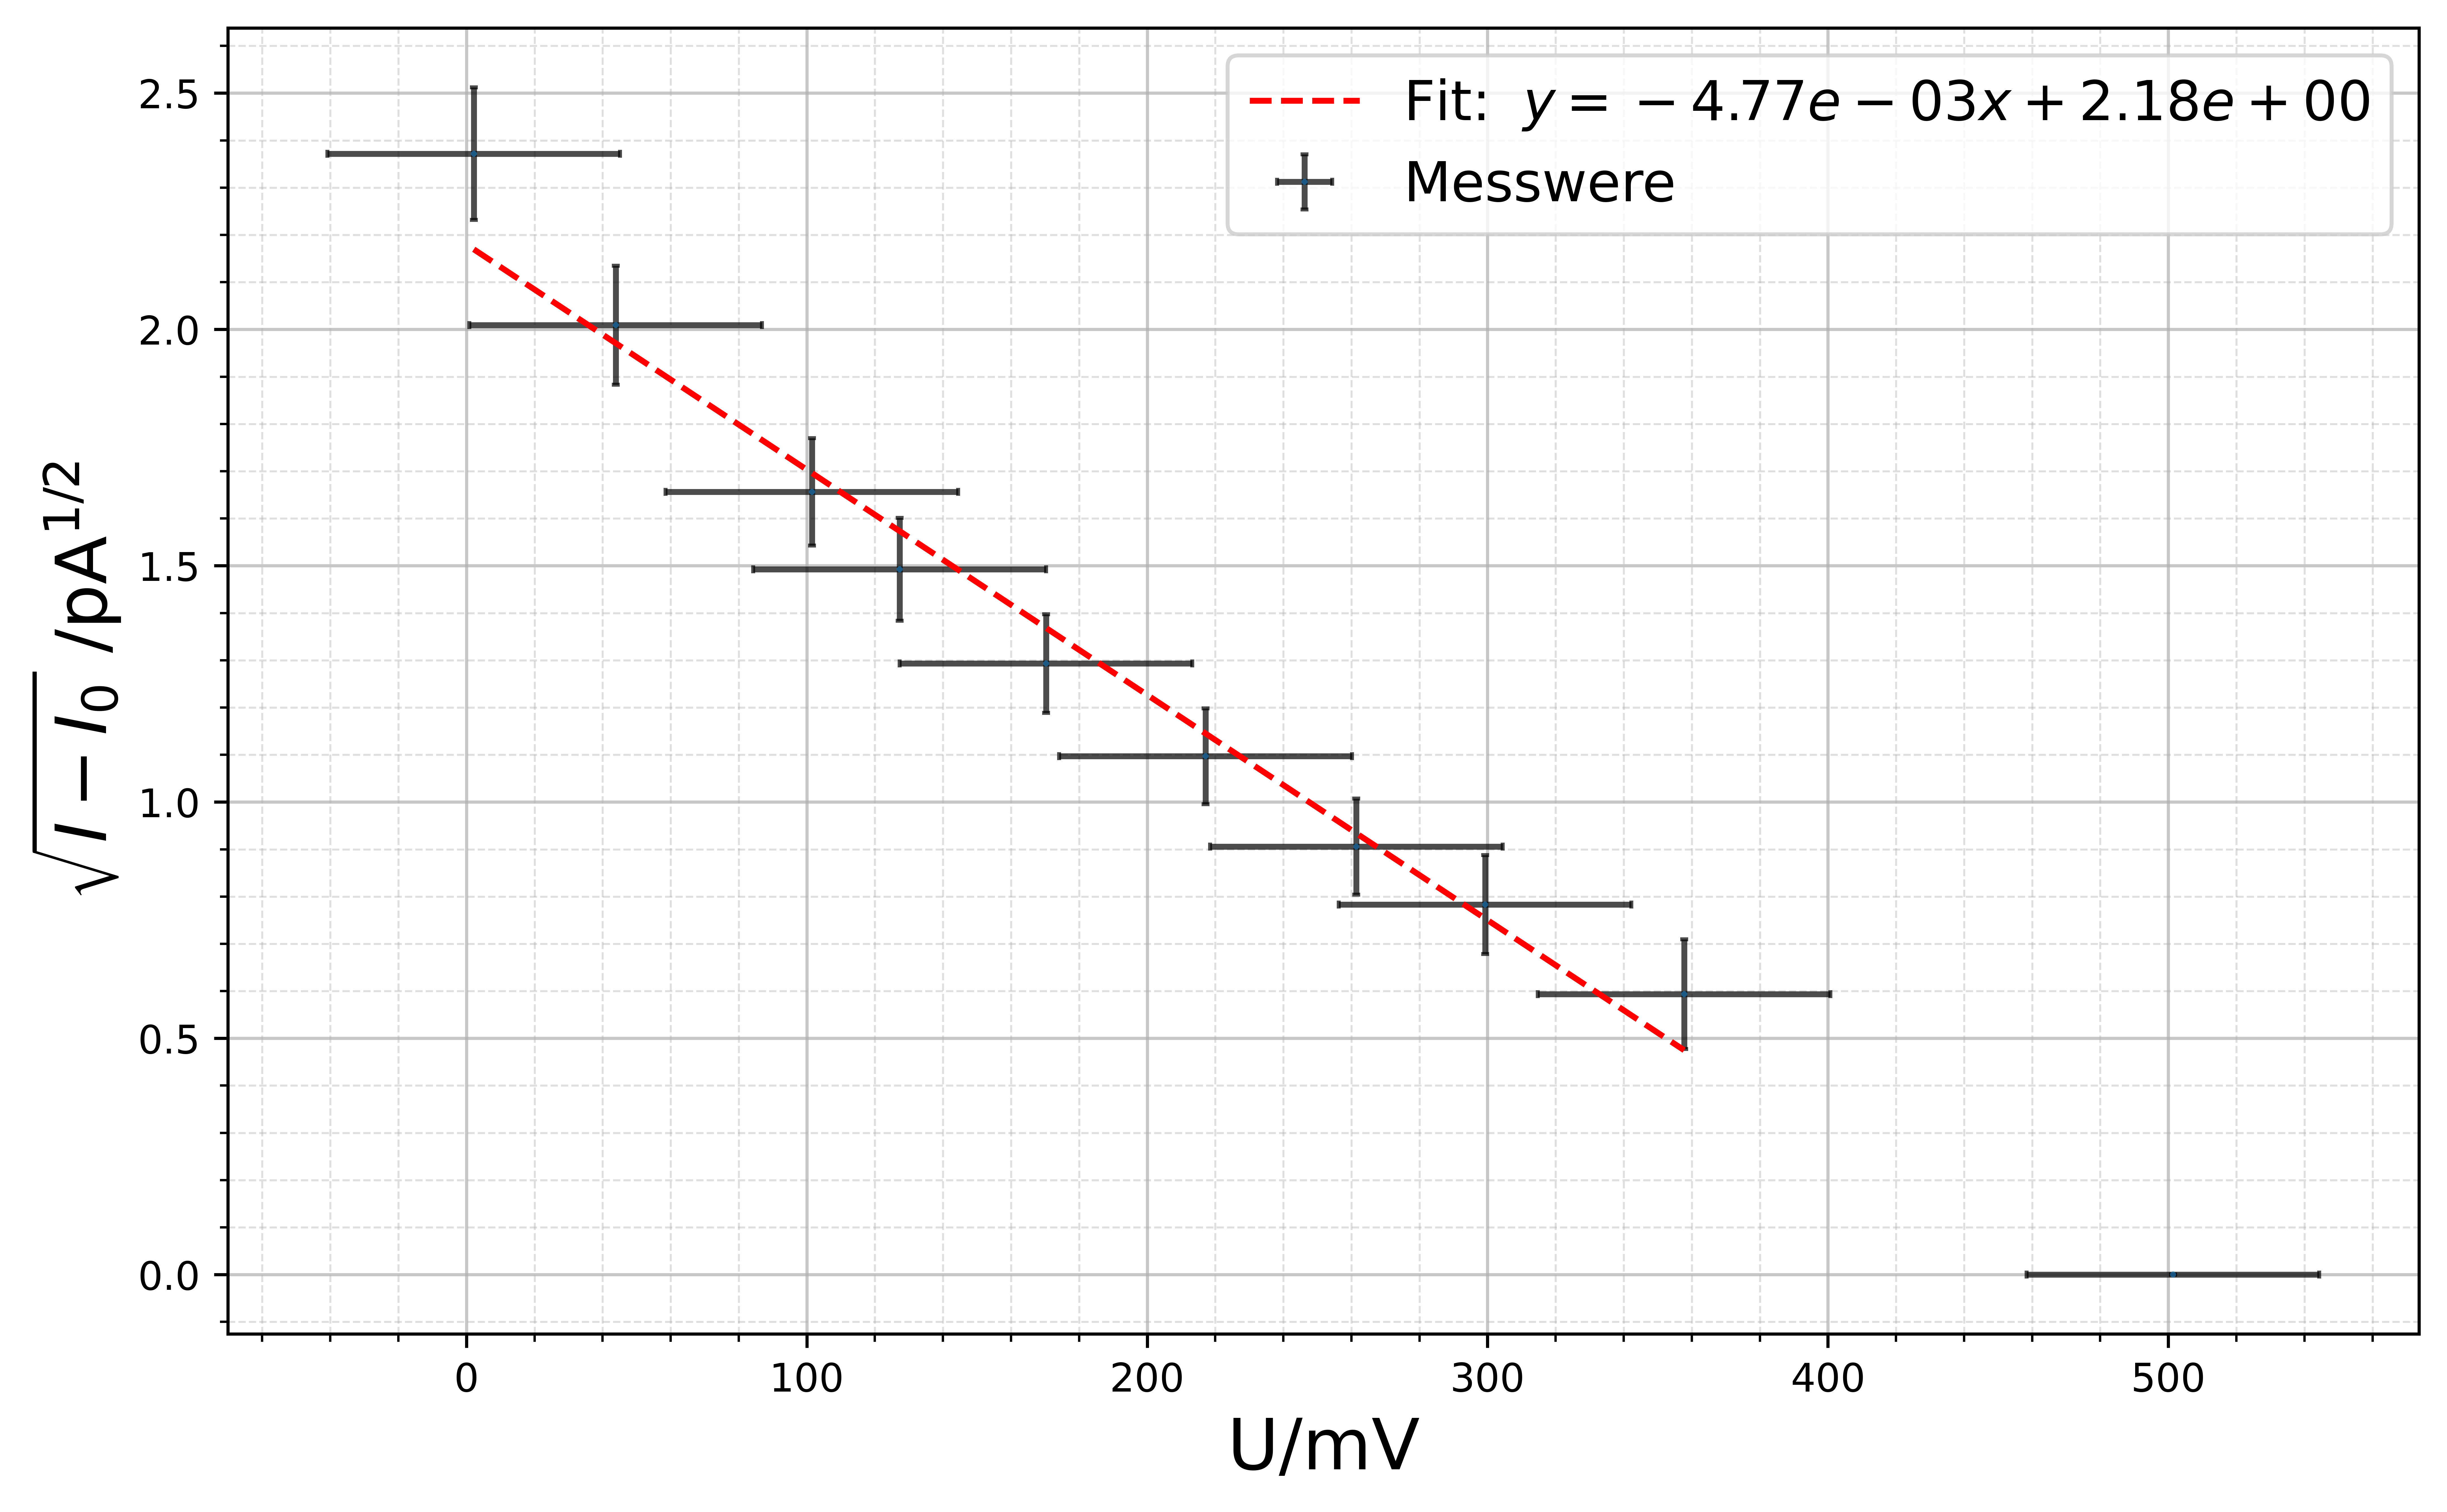
\includegraphics[width=0.95\linewidth]{figs/578_2.png}
    \captionof{figure}{%
      Messung 2 bei $\lambda=\SI{578}{\nm}$. 
      Die Werte und Unsicherheiten sind in \cref{tab:578_second}.%
    }
    \label{fig:578_second}
  \end{minipage}
\end{figure}

\subsection*{Balmer Serie}

\section{Tabellen}
\subsection*{Photoeffekt}
%=======================================================================================================================================================================================================
\begin{table}[H]
\centering
\resizebox{\columnwidth}{!}{
\begin{tabular}{|c|c|c|c|c|c|c|c|}
\hline
\multicolumn{4}{|c|}{$\lambda = \SI{365}{\nm}$}
  & \multicolumn{4}{c|}{$\lambda = \SI{405}{\nm}$} \\ \hline
\multicolumn{2}{|c|}{Messung 1} & \multicolumn{2}{c|}{Messung 2}
  & \multicolumn{2}{c|}{Messung 1} & \multicolumn{2}{c|}{Messung 2} \\ \hline
$U_G {[\si{mV}]}$   & $U_{ph} {[\si{mV}]}$  & $U_G {[\si{mV}]}$  & $U_{ph} {[\si{mV}]}$ & $U_G {[\si{mV}]}$    & $U_{ph} {[\si{mV}]}$ & $U_G {[\si{mV}]}$  & $U_{ph} {[\si{mV}]}$ \\ \hline
0,5             & 2380,0            & 0,5           & 2382,0           & 0,5             & 900,0            & 0,5           & 914,0            \\ \hline
30,5            & 2070,0            & 35,6          & 2065,0           & 41,5            & 722,0            & 36,0            & 740,0            \\ \hline
84,2            & 1630,0            & 84,6          & 1624,0           & 49,4            & 680,0            & 53,9          & 665,0            \\ \hline
121,0             & 1325,0            & 120,5         & 1334,0           & 105,4           & 450,0            & 102,0           & 464,0            \\ \hline
152,9           & 1071,0            & 156,3         & 1061,0           & 149,6           & 293,8          & 152,9         & 286,9,0          \\ \hline
160,7           & 1025,0            & 170,3         & 951,0            & 167,7           & 245,0            & 165,6         & 250,5          \\ \hline
182,4           & 883,0             & 180,8         & 892,0            & 174,5           & 226,9          & 178,2         & 215,6          \\ \hline
190,7           & 823,0             & 194,8         & 795,0            & 201,7           & 161,2          & 200,3         & 164,8          \\ \hline
217,9           & 655,0             & 219,4         & 653,0            & 213,7           & 139,5          & 217,5         & 230,0            \\ \hline
270,0             & 396,0             & 271,1         & 392,0            & 247,4           & 86,1           & 254,1         & 78,8           \\ \hline
287,0             & 333,3           & 287,4         & 325,0            & 267,7           & 63,5           & 273,2         & 58,2           \\ \hline
355,7           & 152,7           & 359,2         & 148,8          & 289,6           & 45,8           & 293,0           & 24,8           \\ \hline
396,3           & 79,9            & 397,2         & 95,6           & 301,9           & 38,8           & 304,7         & 36,5           \\ \hline
452,0             & 32,9            & 455,0           & 29,2           & 352,9           & 14,8           & 345,3         & 17,6           \\ \hline
472,0             & 14,1            & 477,0          & 11,7           & 378,1           & 5,1            & 384,8         & 3,2            \\ \hline
517,0             & 1,1             & 516,0           & 1,4            & 410,0             & 1,1            & 405,0           & 1,1            \\ \hline
\end{tabular}%
}
\caption{Messwerte der Photospannung $U_{ph}$ bei Gegenspannung $U_G$ für $\lambda$ = $\SI{365}{\nm}$ und $\lambda$ = $\SI{405}{\nm}$, wobei $\Delta U_{ph} = 0.1 \cdot U_{ph} + 10\,\si{\milli\volt}, \quad
 \Delta U_{G} = 10 \si{\milli\volt}$}
\label{tab:365and405}
\end{table}
%=======================================================================================================================================================================================================

\begin{table}[H]
\centering
\resizebox{0.5\columnwidth}{!}{%
  \begin{tabular}{|c|c|c|c|}
    \hline
    \multicolumn{4}{|c|}{$\lambda = \SI{463}{\nm}$} \\ \hline
    \multicolumn{2}{|c|}{Messung 1} & \multicolumn{2}{c|}{Messung 2} \\ \hline
    $U_G {[\si{mV}]}$ & $U_{ph} {[\si{mV}]}$ & $U_G {[\si{mV}]}$ & $U_{ph} {[\si{mV}]}$ \\ \hline
    0,5   & 1107,0   & 0,5   & 1130,0   \\ \hline
    31,1  & 901,0    & 34,3  & 866,0    \\ \hline
    87,5  & 537,0    & 91,9  & 522,0    \\ \hline
    133,2 & 313,1    & 135,0 & 307,4    \\ \hline
    152,1 & 236,9    & 152,1 & 242,8    \\ \hline
    192,5 & 126,6    & 190,6 & 130,0    \\ \hline
    227,5 & 68,5     & 227,0 & 68,8     \\ \hline
    291,0 & 18,8     & 287,4 & 21,1     \\ \hline
    334,9 & 1,9      & 329,2 & 2,8      \\ \hline
    345,9 & 0,6      & 349,4 & 0,0      \\ \hline
  \end{tabular}%
}
\caption{Messwerte der Photospannung $U_{ph}$ bei Gegenspannung $U_G$ für $\lambda = \SI{463}{\nm}$, mit $\Delta U_{ph} = 0.1 \cdot U_{ph} + \SI{10}{\milli\volt}$ und $\Delta U_{G} = \SI{10}{\milli\volt}$.}
\label{tab:463nm}
\end{table}
%=======================================================================================================================================================================================================
\begin{table}[H]
\centering
\resizebox{\columnwidth}{!}{%
  \begin{tabular}{|c|c|c|c|c|c|c|c|}
    \hline
    \multicolumn{4}{|c|}{$\lambda = \SI{546}{\nm}$}
      & \multicolumn{4}{c|}{$\lambda = \SI{578}{\nm}$} \\ \hline
    \multicolumn{2}{|c|}{Messung 1} & \multicolumn{2}{c|}{Messung 2}
      & \multicolumn{2}{c|}{Messung 1} & \multicolumn{2}{c|}{Messung 2} \\ \hline
    $U_G {[\si{mV}]}$ & $U_{ph} {[\si{mV}]}$ & $U_G {[\si{mV}]}$ & $U_{ph} {[\si{mV}]}$
      & $U_G {[\si{mV}]}$ & $U_{ph} {[\si{mV}]}$ & $U_G {[\si{mV}]}$ & $U_{ph} {[\si{mV}]}$ \\ \hline
    0,5   & 5700,0   & 0,5   & 5390,0
      & 0,5   & 644,0    & 0,5   & 565,0    \\ \hline
    32,7  & 2155,0   & 29,0  & 2444,0
      & 10,7  & 406,0    & 10,2  & 406,0    \\ \hline
    12,4  & 3900,0   & 9,1   & 4230,0
      & 21,6  & 287,5    & 23,6  & 276,8    \\ \hline
    52,9  & 1165,0   & 51,0  & 1206,0
      & 31,1  & 217,2    & 29,6  & 225,1    \\ \hline
    69,9  & 677,0    & 61,7  & 874,0
      & 39,6  & 169,3    & 39,6  & 169,6    \\ \hline
    60,4  & 949,0    & 71,8  & 645,0
      & 54,9  & 117,2    & 50,5  & 122,7    \\ \hline
    103,2 & 212,9    & 101,0 & 242,1
      & 62,1  & 82,6     & 60,8  & 84,4     \\ \hline
    130,7 & 77,7     & 128,7 & 82,2
      & 73,3  & 55,7     & 69,6  & 63,7     \\ \hline
    150,8 & 13,8     & 150,8 & 18,3
      & 82,2  & 39,6     & 83,2  & 37,6     \\ \hline
    162,4 & 6,2      & 158,7 & 0,1
      & 119,8 & 0,0      & 116,6 & 2,4      \\ \hline
  \end{tabular}%
}
\caption{Messwerte der Photospannung $U_{ph}$ bei Gegenspannung $U_G$ für $\lambda = \SI{546}{\nm}$ und $\lambda = \SI{578}{\nm}$, wobei $\Delta U_{ph} = 0.1 \cdot U_{ph} + \SI{10}{\milli\volt}$ und $\Delta U_{G} = \SI{10}{\milli\volt}$.}
\label{tab:546and578}
\end{table}
%=======================================================================================================================================================================================================
\begin{table}[H]
\centering
\resizebox{0.5\columnwidth}{!} \\ \hline
    $U_G {[\si{mV}]}$ & $U_{ph} {[\si{mV}]}$ & $U_G {[\si{mV}]}$ & $U_{ph} {[\si{mV}]}$ \\ \hline
    0,4    & 9200,0 & 0,5   & 4040,0 \\ \hline
    100,2  & 5760,0 & 106,6 & 2417,0 \\ \hline
    200,8  & 2939,0 & 203,3 & 1296,0 \\ \hline
    259,3  & 1806,0 & 235,6 &  974,0 \\ \hline
    299,3  & 1172,0 & 255,8 &  806,0 \\ \hline
    330,4  &  823,0 & 279,8 &  630,0 \\ \hline
    364,5  &  549,0 & 303,6 &  491,0 \\ \hline
    402,0  &  337,6 & 350,8 &  282,4 \\ \hline
    453,0  &  111,6 & 404,0 &  147,8 \\ \hline
    504,0  &   12,2 & 450,0 &   58,8 \\ \hline
    1020,0 &    1,5 & 510,0 &   10,0 \\ \hline
  \end{tabular}%
}
\caption{Messwerte der Photospannung $U_{ph}$ bei Gegenspannung $U_G$ für $\lambda = \SI{365}{\nm}$ (Maximalwerte und 50\%-Punkt), wobei $\Delta U_{ph} = 0.1 \cdot U_{ph} + \SI{10}{\milli\volt}$ und $\Delta U_{G} = \SI{10}{\milli\volt}$.}
\label{tab:365_max_50}
\end{table}
%=======================================================================================================================================================================================================
\begin{table}[H]
\centering
\resizebox{0.75\columnwidth}{!}{%
\begin{tabular}{|c|c|c|c|c|c|}
\hline
$U$ [\si{\milli\volt}] & $\Delta U$ [\si{\milli\volt}] 
  & $I$ [\si{\pico\ampere}] & $\Delta I$ [\si{\pico\ampere}] 
  & $\sqrt{I - I_0}$ [\si{\sqrt{\pico\ampere}}] 
  & $\Delta\sqrt{I - I_0}$ [\si{\sqrt{\pico\ampere}}] \\ \hline
   2.15 &  43.00 & 2380.00 & 248.00 &  48.77 & 2.54 \\ \hline
 131.15 &  43.00 & 2070.00 & 217.00 &  45.49 & 2.39 \\ \hline
 362.06 &  43.00 & 1630.00 & 173.00 &  40.36 & 2.14 \\ \hline
 520.30 &  43.00 & 1325.00 & 142.50 & 36.39 & 1.96 \\ \hline
 657.47 &  43.00 & 1071.00 & 117.10 & 32.71 & 1.79 \\ \hline
 691.01 &  43.00 & 1025.00 & 112.50 & 32.00 & 1.76 \\ \hline
 784.32 &  43.00 &  883.00 &  98.30 & 29.70 & 1.66 \\ \hline
 820.01 &  43.00 &  823.00 &  92.30 & 28.67 & 1.61 \\ \hline
 936.97 &  43.00 &  655.00 &  75.50 & 25.57 & 1.48 \\ \hline
1161.00 &  43.00 &  396.00 &  49.60 & 19.87 & 1.25 \\ \hline
1234.10 &  43.00 &  333.30 &  43.33 & 18.23 & 1.19 \\ \hline
1529.51 &  43.00 &  152.70 &  25.27 & 12.31 & 1.03 \\ \hline
1704.09 &  43.00 &   79.90 &  17.99 &  8.88 & 1.01 \\ \hline
1943.60 &  43.00 &   32.90 &  13.29 &  5.64 & 1.18 \\ \hline
2029.60 &  43.00 &   14.10 &  11.41 &  3.61 & 1.58 \\ \hline
2223.10 &  43.00 &    1.10 &  10.11 &  0.00 & 0.00 \\ \hline
\end{tabular}%
}
\caption{Gemessenen Werte für die erste Messung bei $\lambda=\SI{365}{\nano\metre}$.  
Die Sättigungsspannung liegt bei $U_G= \SI{517.00}{\milli\volt}$, daraus folgt  
$I_0 = \SI{1.10 \pm 10.11}{\pico\ampere}$.}
\label{tab:365_first}
\end{table}

\begin{table}[H]
\centering
\resizebox{0.75\columnwidth}{!}{%
\begin{tabular}{|c|c|}
\hline
\textbf{Parameter} & \textbf{Wert} \\ \hline
Steigung $m$ [\si{\sqrt{\pico\ampere}/\milli\volt}]
  & $\num{-2.22e-2} \pm \num{5.58e-4}$ \\ \hline
Achsenabschnitt $b$ [\si{\sqrt{\pico\ampere}}]
  & $\num{4.70e1} \pm \num{7.48e-1}$ \\ \hline
$\mathrm{\chi}^2$
  & $\num{8.28}$ \\ \hline
Freiheitsgrade (dof)
  & 13 \\ \hline
$\mathrm{\chi}^2 / \mathrm{dof}$
  & $\num{0.637}$ \\ \hline
Abbrems­spannung $U_0$ [\si{\milli\volt}]
  & $\num{2117.12 \pm 62.98}$ \\ \hline
\end{tabular}%
}
\caption{Ergebnisse des gewichteten linearen $\mathrm{\chi}^2$-Fits zur Bestimmung der Abbrems­spannung für die erste Messung bei $\lambda=\SI{365}{\nano\metre}$. Die hier gezeigten Werte stammen aus Tabelle \ref{tab:365_first}.}
\label{tab:365_first_chi2}
\end{table}

%=======================================================================================================================================================================================================

\begin{table}[H]
\centering
\resizebox{0.75\columnwidth}{!}{%
\begin{tabular}{|c|c|c|c|c|c|}
\hline
$U$ [\si{\milli\volt}] & $\Delta U$ [\si{\milli\volt}] 
  & $I$ [\si{\pico\ampere}] & $\Delta I$ [\si{\pico\ampere}] 
  & $\sqrt{I - I_0}$ [\si{\sqrt{\pico\ampere}}] 
  & $\Delta\sqrt{I - I_0}$ [\si{\sqrt{\pico\ampere}}] \\ \hline
   2.15 &  43.00 & 2382.00 & 248.20 &  48.79 &  2.54 \\ \hline
 153.08 &  43.00 & 2065.00 & 216.50 &  45.43 &  2.38 \\ \hline
 363.78 &  43.00 & 1624.00 & 172.40 &  40.28 &  2.14 \\ \hline
 518.15 &  43.00 & 1334.00 & 143.40 &  36.50 &  1.96 \\ \hline
 672.09 &  43.00 & 1061.00 & 116.10 &  32.55 &  1.78 \\ \hline
 732.29 &  43.00 &  951.00 & 105.10 &  30.82 &  1.71 \\ \hline
 777.44 &  43.00 &  892.00 &  99.20 &  29.84 &  1.66 \\ \hline
 837.64 &  43.00 &  795.00 &  89.50 &  28.17 &  1.59 \\ \hline
 943.42 &  43.00 &  653.00 &  75.30 &  25.53 &  1.47 \\ \hline
1165.73 &  43.00 &  392.00 &  49.20 &  19.76 &  1.24 \\ \hline
1235.82 &  43.00 &  325.00 &  42.50 &  17.99 &  1.18 \\ \hline
1544.56 &  43.00 &  148.80 &  24.88 &  12.14 &  1.02 \\ \hline
1707.96 &  43.00 &   95.60 &  19.56 &   9.71 &  1.01 \\ \hline
1956.50 &  43.00 &   29.20 &  12.92 &   5.27 &  1.23 \\ \hline
2051.10 &  43.00 &   11.70 &  11.17 &   3.21 &  1.74 \\ \hline
2218.80 &  43.00 &    1.40 &  10.14 &   0.00 &  0.00 \\ \hline
\end{tabular}%
}
\caption{Gemessenen Werte für die zweite Messung bei $\lambda=\SI{365}{\nano\metre}$.  
Die Sättigungsspannung liegt bei $U_G=\SI{516.00}{\milli\volt}$, daraus folgt  
$I_0 = \SI[separate-uncertainty=true]{1.40 \pm 10.14}{\pico\ampere}$.}
\label{tab:365_second}
\end{table}

\begin{table}[H]
\centering
\resizebox{0.75\columnwidth}{!}{%
\begin{tabular}{|c|c|}
\hline
\textbf{Parameter} & \textbf{Wert} \\ \hline
Steigung $m$ [\si{\sqrt{\pico\ampere}/\milli\volt}] 
  & $\num{-2.20e-2} \pm \num{5.73e-4}$ \\ \hline
Achsenabschnitt $b$ [\si{\sqrt{\pico\ampere}}] 
  & $\num{4.69e1} \pm \num{7.63e-1}$ \\ \hline
$\mathrm{\chi}^2$ 
  & $\num{8.45}$ \\ \hline
Freiheitsgrade (dof) 
  & 13 \\ \hline
$\mathrm{\chi}^2 / \mathrm{dof}$ 
  & $\num{0.650}$ \\ \hline
Abbrems­spannung $U_0$ [\si{\milli\volt}] 
  & $\num{2131.82 \pm 65.47}$ \\ \hline
\end{tabular}%
}
\caption{Ergebnisse des gewichteten linearen $\mathrm{\chi}^2$-Fits zur Bestimmung der Abbrems­spannung für die zweite Messung bei $\lambda=\SI{365}{\nano\metre}$. Die hier gezeigten Werte stammen aus Tabelle \ref{tab:365_second}.}
\label{tab:365_second_chi2}
\end{table}


%=======================================================================================================================================================================================================
\begin{table}[H]
\centering
\resizebox{0.75\columnwidth}{!}{%
\begin{tabular}{|c|c|c|c|c|c|}
\hline
$U$ [\si{\milli\volt}] & $\Delta U$ [\si{\milli\volt}] 
  & $I$ [\si{\pico\ampere}] & $\Delta I$ [\si{\pico\ampere}] 
  & $\sqrt{I - I_0}$ [\si{\sqrt{\pico\ampere}}] 
  & $\Delta\sqrt{I - I_0}$ [\si{\sqrt{\pico\ampere}}] \\ \hline
   2.15 &  43.00 & 4040.00 & 414.00 &  63.48 & 3.26 \\ \hline
 458.38 &  43.00 & 2417.00 & 251.70 &  49.06 & 2.57 \\ \hline
 874.19 &  43.00 & 1296.00 & 139.60 &  35.86 & 1.95 \\ \hline
1013.08 &  43.00 &  974.00 & 107.40 &  31.05 & 1.73 \\ \hline
1099.94 &  43.00 &  806.00 &  90.60 &  28.21 & 1.61 \\ \hline
1203.14 &  43.00 &  630.00 &  73.00 &  24.90 & 1.47 \\ \hline
1305.48 &  43.00 &  491.00 &  59.10 &  21.93 & 1.35 \\ \hline
1508.44 &  43.00 &  282.40 &  38.24 &  16.50 & 1.16 \\ \hline
1737.20 &  43.00 &  147.80 &  24.78 &  11.74 & 1.06 \\ \hline
1935.00 &  43.00 &   58.80 &  15.88 &   6.99 & 1.14 \\ \hline
2193.00 &  43.00 &   10.00 &  11.00 &   0.00 & 0.00 \\ \hline
\end{tabular}%
}
\caption{Gemessenen Werte für die Messung bei 50 \% Intensität und $\lambda=\SI{365}{\nano\metre}$.  
Die Sättigungsspannung liegt bei $U_G=\SI{510.00}{\milli\volt}$, daraus folgt  
$I_0 = \SI[separate-uncertainty=true]{10.00 \pm 11.00}{\pico\ampere}$.}
\label{tab:365_50pct}
\end{table}

\begin{table}[H]
\centering
\resizebox{0.75\columnwidth}{!}{%
\begin{tabular}{|c|c|}
\hline
\textbf{Parameter} & \textbf{Wert} \\ \hline
Steigung $m$ [\si{\sqrt{\pico\ampere}/\milli\volt}] 
  & $\num{-2.79e-2} \pm \num{9.92e-4}$ \\ \hline
Achsenabschnitt $b$ [\si{\sqrt{\pico\ampere}}] 
  & $\num{5.96e1} \pm \num{1.45e0}$ \\ \hline
$\mathrm{\chi}^2$ 
  & $\num{6.55}$ \\ \hline
Freiheitsgrade (dof) 
  & 8 \\ \hline
$\mathrm{\chi}^2 / \mathrm{dof}$ 
  & $\num{0.819}$ \\ \hline
Abbrems­spannung $U_0$ [\si{\milli\volt}] 
  & $\num{2136.20 \pm 92.03}$ \\ \hline
\end{tabular}%
}
\caption{Ergebnisse des gewichteten linearen $\mathrm{\chi}^2$-Fits zur Bestimmung der Abbrems­spannung für die Messung bei $\lambda=\SI{365}{\nano\metre}$ mit 50\% Intensität. Die hier gezeigten Werte stammen aus Tabelle \ref{tab:365_50pct}.}
\label{tab:365_50_chi2}
\end{table}

%=======================================================================================================================================================================================================
\begin{table}[H]
\centering
\resizebox{0.75\columnwidth}{!}{%
\begin{tabular}{|c|c|c|c|c|c|}
\hline
$U$ [\si{\milli\volt}] & $\Delta U$ [\si{\milli\volt}] 
  & $I$ [\si{\pico\ampere}] & $\Delta I$ [\si{\pico\ampere}] 
  & $\sqrt{I - I_0}$ [\si{\sqrt{\pico\ampere}}] 
  & $\Delta\sqrt{I - I_0}$ [\si{\sqrt{\pico\ampere}}] \\ \hline
   1.72 &  43.00 & 9200.00 &  930.00 &  95.91 & 4.85 \\ \hline
 430.86 &  43.00 & 5760.00 &  586.00 &  75.88 & 3.86 \\ \hline
 863.44 &  43.00 & 2939.00 &  303.90 &  54.20 & 2.80 \\ \hline
1114.99 &  43.00 & 1806.00 &  190.60 &  42.48 & 2.24 \\ \hline
1286.99 &  43.00 & 1172.00 &  127.20 &  34.21 & 1.86 \\ \hline
1420.72 &  43.00 &  823.00 &   92.30 &  28.66 & 1.61 \\ \hline
1567.35 &  43.00 &  549.00 &   64.90 &  23.40 & 1.39 \\ \hline
1728.60 &  43.00 &  337.60 &   43.76 &  18.33 & 1.19 \\ \hline
1947.90 &  43.00 &  111.60 &   21.16 &  10.49 & 1.01 \\ \hline
2167.20 &  43.00 &   12.20 &   11.22 &   3.27 & 1.72 \\ \hline
4386.00 &  43.00 &    1.50 &   10.15 &   0.00 & 0.00 \\ \hline
\end{tabular}%
}
\caption{Gemessenen Werte für die Messung bei maximaler Intensität und $\lambda=\SI{365}{\nano\metre}$.  
Die Sättigungsspannung liegt bei $U_G=\SI{1020.00}{\milli\volt}$, daraus folgt  
$I_0 = \SI[separate-uncertainty=true]{1.50 \pm 10.15}{\pico\ampere}$.}
\label{tab:365_max}
\end{table}

\begin{table}[H]
\centering
\resizebox{0.75\columnwidth}{!}{%
\begin{tabular}{|c|c|}
\hline
\textbf{Parameter} & \textbf{Wert} \\ \hline
Steigung $m$ [\si{\sqrt{\pico\ampere}/\milli\volt}] 
  & $\num{-4.00e-2} \pm \num{1.57e-3}$ \\ \hline
Achsenabschnitt $b$ [\si{\sqrt{\pico\ampere}}] 
  & $\num{8.76e1} \pm \num{2.64e0}$ \\ \hline
$\mathrm{\chi}^2$ 
  & $\num{11.74}$ \\ \hline
Freiheitsgrade (dof) 
  & 8 \\ \hline
$\mathrm{\chi}^2 / \mathrm{dof}$ 
  & $\num{1.467}$ \\ \hline
Abbrems­spannung $U_0$ [\si{\milli\volt}] 
  & $\num{2190.00 \pm 108.37}$ \\ \hline
\end{tabular}%
}
\caption{Ergebnisse des gewichteten linearen $\mathrm{\chi}^2$-Fits zur Bestimmung der Abbrems­spannung für die Messung bei $\lambda=\SI{365}{\nano\metre}$ mit maximaler Intensität. Die hier gezeigten Werte stammen aus Tabelle \ref{tab:365_max}.}
\label{tab:365_max_chi2}
\end{table}

%=======================================================================================================================================================================================================
\begin{table}[H]
\centering
\resizebox{0.75\columnwidth}{!}{%
\begin{tabular}{|c|c|c|c|c|c|}
\hline
$U$ [\si{\milli\volt}] & $\Delta U$ [\si{\milli\volt}] 
  & $I$ [\si{\pico\ampere}] & $\Delta I$ [\si{\pico\ampere}] 
  & $\sqrt{I - I_0}$ [\si{\sqrt{\pico\ampere}}] 
  & $\Delta\sqrt{I - I_0}$ [\si{\sqrt{\pico\ampere}}] \\ \hline
   2.15 &  43.00 &  900.00 & 100.00 &  29.98 & 1.67 \\ \hline
 178.45 &  43.00 &  722.00 &  82.20 &  26.85 & 1.53 \\ \hline
 212.42 &  43.00 &  680.00 &  78.00 &  26.06 & 1.50 \\ \hline
 453.22 &  43.00 &  450.00 &  55.00 &  21.19 & 1.30 \\ \hline
 643.28 &  43.00 &  293.80 &  39.38 &  17.11 & 1.15 \\ \hline
 721.11 &  43.00 &  245.00 &  34.50 &  15.62 & 1.10 \\ \hline
 750.35 &  43.00 &  226.90 &  32.69 &  15.03 & 1.09 \\ \hline
 867.31 &  43.00 &  161.20 &  26.12 &  12.65 & 1.03 \\ \hline
 918.91 &  43.00 &  139.50 &  23.95 &  11.76 & 1.02 \\ \hline
1063.82 &  43.00 &   86.10 &  18.61 &   9.22 & 1.01 \\ \hline
1151.11 &  43.00 &   63.50 &  16.35 &   7.90 & 1.03 \\ \hline
1245.28 &  43.00 &   45.80 &  14.58 &   6.69 & 1.09 \\ \hline
1298.17 &  43.00 &   38.80 &  13.88 &   6.14 & 1.13 \\ \hline
1517.47 &  43.00 &   14.80 &  11.48 &   3.70 & 1.55 \\ \hline
1625.83 &  43.00 &    5.10 &  10.51 &   2.00 & 2.63 \\ \hline
1763.00 &  43.00 &    1.10 &  10.11 &   0.00 & 0.00 \\ \hline
\end{tabular}%
}
\caption{Gemessenen Werte für die erste Messung bei $\lambda=\SI{405}{\nano\metre}$.  
Die Sättigungsspannung liegt bei $U_G=\SI{410.00}{\milli\volt}$, daraus folgt  
$I_0 = \SI[separate-uncertainty=true]{1.10 \pm 10.11}{\pico\ampere}$.}
\label{tab:405_first}
\end{table}

\begin{table}[H]
\centering
\resizebox{0.75\columnwidth}{!}{%
\begin{tabular}{|c|c|}
\hline
\textbf{Parameter} & \textbf{Wert} \\ \hline
Steigung $m$ [\si{\sqrt{\pico\ampere}/\milli\volt}] 
  & $\num{-1.81e-2} \pm \num{5.50e-4}$ \\ \hline
Achsenabschnitt $b$ [\si{\sqrt{\pico\ampere}}] 
  & $\num{2.90e1} \pm \num{5.21e-1}$ \\ \hline
$\mathrm{\chi}^2$ 
  & $\num{5.80}$ \\ \hline
Freiheitsgrade (dof) 
  & 13 \\ \hline
$\mathrm{\chi}^2 / \mathrm{dof}$ 
  & $\num{0.446}$ \\ \hline
Abbrems­spannung $U_0$ [\si{\milli\volt}] 
  & $\num{1602.21 \pm 56.56}$ \\ \hline
\end{tabular}%
}
\caption{Ergebnisse des gewichteten linearen $\mathrm{\chi}^2$-Fits zur Bestimmung der Abbrems­spannung für die erste Messung bei $\lambda=\SI{405}{\nano\metre}$. Die hier gezeigten Werte stammen aus Tabelle \ref{tab:405_first}.}
\label{tab:405_first_chi2}
\end{table}

%=======================================================================================================================================================================================================
\begin{table}[H]
\centering
\resizebox{0.75\columnwidth}{!}{%
  \begin{tabular}{|c|c|c|c|c|c|}
    \hline
    $U$ [\si{\milli\volt}] & $\Delta U$ [\si{\milli\volt}]
      & $I$ [\si{\pico\ampere}] & $\Delta I$ [\si{\pico\ampere}]
      & $\sqrt{I - I_0}$ [\si{\sqrt{\pico\ampere}}]
      & $\Delta\sqrt{I - I_0}$ [\si{\sqrt{\pico\ampere}}] \\ \hline
       2.15 &  43.00 &  914.00 & 101.40 &  30.21 & 1.68 \\ \hline
 154.80 &  43.00 &  740.00 &  84.00 &  27.18 & 1.55 \\ \hline
 231.77 &  43.00 &  665.00 &  76.50 &  25.77 & 1.48 \\ \hline
 438.60 &  43.00 &  464.00 &  56.40 &  21.52 & 1.31 \\ \hline
 657.47 &  43.00 &  286.90 &  38.69 &  16.91 & 1.14 \\ \hline
 712.08 &  43.00 &  250.50 &  35.05 &  15.79 & 1.11 \\ \hline
 766.26 &  43.00 &  215.60 &  31.56 &  14.65 & 1.08 \\ \hline
 861.29 &  43.00 &  164.80 &  26.48 &  12.79 & 1.03 \\ \hline
 935.25 &  43.00 &  230.00 &  33.00 &  15.13 & 1.09 \\ \hline
1092.63 &  43.00 &   78.80 &  17.88 &   8.81 & 1.01 \\ \hline
1174.76 &  43.00 &   58.20 &  15.82 &   7.56 & 1.05 \\ \hline
1259.90 &  43.00 &   24.80 &  12.48 &   4.87 & 1.28 \\ \hline
1310.21 &  43.00 &   36.50 &  13.65 &   5.95 & 1.15 \\ \hline
1484.79 &  43.00 &   17.60 &  11.76 &   4.06 & 1.45 \\ \hline
1654.64 &  43.00 &    3.20 &  10.32 &   1.45 & 3.56 \\ \hline
1741.50 &  43.00 &    1.10 &  10.11 &   0.00 & 0.00 \\ \hline
  \end{tabular}%
}
\caption{Gemessenen Werte für die zweite Messung bei 
  $\lambda=\SI{405}{\nano\metre}$.  
  Die Sättigungsspannung liegt bei $U_G=\SI{405.00}{\milli\volt}$, daraus folgt  
  $I_0 = \SI[separate-uncertainty=true]{1.10 \pm 10.11}{\pico\ampere}$.}
\label{tab:405_second}
\end{table}

\begin{table}[H]
\centering
\resizebox{0.75\columnwidth}{!}{%
\begin{tabular}{|c|c|}
\hline
\textbf{Parameter} & \textbf{Wert} \\ \hline
Steigung $m$ [\si{\sqrt{\pico\ampere}/\milli\volt}] 
  & $\num{-1.83e-2} \pm \num{8.30e-4}$ \\ \hline
Achsenabschnitt $b$ [\si{\sqrt{\pico\ampere}}] 
  & $\num{2.95e1} \pm \num{7.84e-1}$ \\ \hline
$\mathrm{\chi}^2$ 
  & $\num{12.92}$ \\ \hline
Freiheitsgrade (dof) 
  & 13 \\ \hline
$\mathrm{\chi}^2 / \mathrm{dof}$ 
  & $\num{0.994}$ \\ \hline
Abbrems­spannung $U_0$ [\si{\milli\volt}] 
  & $\num{1612.02 \pm 84.74}$ \\ \hline
\end{tabular}%
}
\caption{Ergebnisse des gewichteten linearen $\mathrm{\chi}^2$-Fits zur Bestimmung der Abbrems­spannung für die zweite Messung bei $\lambda=\SI{405}{\nano\metre}$. Die hier gezeigten Werte stammen aus Tabelle \ref{tab:405_second}.}
\label{tab:405_second_chi2}
\end{table}

%=======================================================================================================================================================================================================
\begin{table}[H]
\centering
\resizebox{0.75\columnwidth}{!}{%
\begin{tabular}{|c|c|c|c|c|c|}
\hline
$U$ [\si{\milli\volt}] & $\Delta U$ [\si{\milli\volt}] 
  & $I$ [\si{\pico\ampere}] & $\Delta I$ [\si{\pico\ampere}] 
  & $\sqrt{I - I_0}$ [\si{\sqrt{\pico\ampere}}] 
  & $\Delta\sqrt{I - I_0}$ [\si{\sqrt{\pico\ampere}}] \\ \hline
   2.15 &  43.00 & 1107.00 & 120.70 &  33.26 & 1.81 \\ \hline
 133.73 &  43.00 &  901.00 & 100.10 &  30.01 & 1.67 \\ \hline
 376.25 &  43.00 &  537.00 &  63.70 &  23.16 & 1.38 \\ \hline
 572.76 &  43.00 &  313.10 &  41.31 &  17.68 & 1.17 \\ \hline
 654.03 &  43.00 &  236.90 &  33.69 &  15.37 & 1.10 \\ \hline
 827.75 &  43.00 &  126.60 &  22.66 &  11.22 & 1.01 \\ \hline
 978.25 &  43.00 &   68.50 &  16.85 &   8.24 & 1.02 \\ \hline
1251.30 &  43.00 &   18.80 &  11.88 &   4.27 & 1.39 \\ \hline
1440.07 &  43.00 &    1.90 &  10.19 &   1.14 & 4.47 \\ \hline
1487.37 &  43.00 &    0.60 &  10.06 &   0.00 & 0.00 \\ \hline
\end{tabular}%
}
\caption{Gemessenen Werte für die erste Messung bei $\lambda=\SI{463}{\nano\metre}$.  
Die Sättigungsspannung liegt bei $U_G=\SI{1487.37}{\milli\volt}$, daraus folgt  
$I_0 = \SI[separate-uncertainty=true]{0.60 \pm 10.06}{\pico\ampere}$.}
\label{tab:463_first}
\end{table}


\begin{table}[H]
\centering
\resizebox{0.75\columnwidth}{!}{%
\begin{tabular}{|c|c|}
\hline
\textbf{Parameter} & \textbf{Wert} \\ \hline
Steigung $m$ [\si{\sqrt{\pico\ampere}/\milli\volt}] 
  & $\num{-2.38e-2} \pm \num{1.22e-3}$ \\ \hline
Achsenabschnitt $b$ [\si{\sqrt{\pico\ampere}}] 
  & $\num{3.18e1} \pm \num{9.47e-1}$ \\ \hline
$\mathrm{\chi}^2$ 
  & $\num{6.31}$ \\ \hline
Freiheitsgrade (dof) 
  & 7 \\ \hline
$\mathrm{\chi}^2 / \mathrm{dof}$ 
  & $\num{0.901}$ \\ \hline
Abbrems­spannung $U_0$ [\si{\milli\volt}] 
  & $\num{1336.13 \pm 79.21}$ \\ \hline
\end{tabular}%
}
\caption{Ergebnisse des gewichteten linearen $\mathrm{\chi}^2$-Fits zur Bestimmung der Abbrems­spannung für die erste Messung bei $\lambda=\SI{463}{\nano\metre}$. Die hier gezeigten Werte stammen aus Tabelle \ref{tab:463_first}.}
\label{tab:463_first_chi2}
\end{table}

%=======================================================================================================================================================================================================
\begin{table}[H]
\centering
\resizebox{0.75\columnwidth}{!}{%
\begin{tabular}{|c|c|c|c|c|c|}
\hline
$U$ [\si{\milli\volt}] & $\Delta U$ [\si{\milli\volt}] 
  & $I$ [\si{\pico\ampere}] & $\Delta I$ [\si{\pico\ampere}] 
  & $\sqrt{I - I_0}$ [\si{\sqrt{\pico\ampere}}] 
  & $\Delta\sqrt{I - I_0}$ [\si{\sqrt{\pico\ampere}}] \\ \hline
   2.15 &  43.00 & 1130.00 & 123.00 &  33.62 & 1.83 \\ \hline
 147.49 &  43.00 &  866.00 &  96.60 &  29.43 & 1.64 \\ \hline
 395.17 &  43.00 &  522.00 &  62.20 &  22.85 & 1.36 \\ \hline
 580.50 &  43.00 &  307.40 &  40.74 &  17.53 & 1.16 \\ \hline
 654.03 &  43.00 &  242.80 &  34.28 &  15.58 & 1.10 \\ \hline
 819.58 &  43.00 &  130.00 &  23.00 &  11.40 & 1.01 \\ \hline
 976.10 &  43.00 &   68.80 &  16.88 &   8.29 & 1.02 \\ \hline
1235.82 &  43.00 &   21.10 &  12.11 &   4.59 & 1.32 \\ \hline
1415.56 &  43.00 &    2.80 &  10.28 &   1.67 & 3.08 \\ \hline
1502.42 &  43.00 &    0.01 &  10.00 &   0.00 & 0.00 \\ \hline
\end{tabular}%
}
\caption{Gemessenen Werte für die zweite Messung bei $\lambda=\SI{463}{\nano\metre}$.  
Die Sättigungsspannung liegt bei $U_G=\SI{1502.42}{\milli\volt}$, daraus folgt  
$I_0 = \SI[separate-uncertainty=true]{0.01 \pm 10.00}{\pico\ampere}$.}
\label{tab:463_second}
\end{table}

\begin{table}[H]
\centering
\resizebox{0.75\columnwidth}{!}{%
\begin{tabular}{|c|c|}
\hline
\textbf{Parameter} & \textbf{Wert} \\ \hline
Steigung $m$ [\si{\sqrt{\pico\ampere}/\milli\volt}] 
  & $\num{-2.36e-2} \pm \num{1.26e-3}$ \\ \hline
Achsenabschnitt $b$ [\si{\sqrt{\pico\ampere}}] 
  & $\num{3.18e1} \pm \num{9.94e-1}$ \\ \hline
$\mathrm{\chi}^2$ 
  & $\num{6.97}$ \\ \hline
Freiheitsgrade (dof) 
  & 7 \\ \hline
$\mathrm{\chi}^2 / \mathrm{dof}$ 
  & $\num{0.995}$ \\ \hline
Abbrems­spannung $U_0$ [\si{\milli\volt}] 
  & $\num{1347.46 \pm 83.36}$ \\ \hline
\end{tabular}%
}
\caption{Ergebnisse des gewichteten linearen $\mathrm{\chi}^2$-Fits zur Bestimmung der Abbrems­spannung für die zweite Messung bei $\lambda=\SI{463}{\nano\metre}$. Die hier gezeigten Werte stammen aus Tabelle \ref{tab:463_second}.}
\label{tab:463_second_chi2}
\end{table}

%=======================================================================================================================================================================================================
\begin{table}[H]
\centering
\resizebox{0.75\columnwidth}{!}{%
\begin{tabular}{|c|c|c|c|c|c|}
\hline
$U$ [\si{\milli\volt}] & $\Delta U$ [\si{\milli\volt}] 
  & $I$ [\si{\pico\ampere}] & $\Delta I$ [\si{\pico\ampere}] 
  & $\sqrt{I - I_0}$ [\si{\sqrt{\pico\ampere}}] 
  & $\Delta\sqrt{I - I_0}$ [\si{\sqrt{\pico\ampere}}] \\ \hline
   2.15 &  43.00 &   57.00 &   5.80 &   7.55 & 0.38 \\ \hline
 140.61 &  43.00 &   21.55 &   2.25 &   4.64 & 0.24 \\ \hline
  53.32 &  43.00 &   39.00 &   4.00 &   6.24 & 0.32 \\ \hline
 227.47 &  43.00 &   11.65 &   1.26 &   3.40 & 0.19 \\ \hline
 300.57 &  43.00 &    6.77 &   0.78 &   2.59 & 0.15 \\ \hline
 259.72 &  43.00 &    9.49 &   1.05 &   3.07 & 0.17 \\ \hline
 443.76 &  43.00 &    2.13 &   0.31 &   1.44 & 0.11 \\ \hline
 562.01 &  43.00 &    0.78 &   0.18 &   0.85 & 0.11 \\ \hline
 648.44 &  43.00 &    0.14 &   0.11 &   0.28 & 0.21 \\ \hline
 698.32 &  43.00 &    0.06 &   0.11 &   0.00 & 0.00 \\ \hline
\end{tabular}%
}
\caption{Gemessenen Werte für die erste Messung bei $\lambda=\SI{546}{\nano\metre}$.  
Die Sättigungsspannung liegt bei $U_G=\SI{698.32}{\milli\volt}$, daraus folgt  
$I_0 = \SI[separate-uncertainty=true]{0.06 \pm 0.11}{\pico\ampere}$.}
\label{tab:546_first}
\end{table}

\begin{table}[H]
\centering
\resizebox{0.75\columnwidth}{!}{%
\begin{tabular}{|c|c|}
\hline
\textbf{Parameter} & \textbf{Wert} \\ \hline
Steigung $m$ [\si{\sqrt{\pico\ampere}/\milli\volt}] 
  & $\num{-9.06e-3} \pm \num{9.59e-4}$ \\ \hline
Achsenabschnitt $b$ [\si{\sqrt{\pico\ampere}}] 
  & $\num{5.71e0} \pm \num{4.14e-1}$ \\ \hline
$\mathrm{\chi}^2$ 
  & $\num{60.11}$ \\ \hline
Freiheitsgrade (dof) 
  & 7 \\ \hline
$\mathrm{\chi}^2 / \mathrm{dof}$ 
  & $\num{8.587}$ \\ \hline
Abbrems­spannung $U_0$ [\si{\milli\volt}] 
  & $\num{630.24 \pm 80.86}$ \\ \hline
\end{tabular}%
}
\caption{Ergebnisse des gewichteten linearen $\mathrm{\chi}^2$-Fits zur Bestimmung der Abbrems­spannung für die erste Messung bei $\lambda=\SI{546}{\nano\metre}$. Die hier gezeigten Werte stammen aus Tabelle \ref{tab:546_first}.}
\label{tab:546_first_chi2}
\end{table}


%=======================================================================================================================================================================================================
\begin{table}[H]
\centering
\resizebox{0.75\columnwidth}{!}{%
\begin{tabular}{|c|c|c|c|c|c|}
\hline
$U$ [\si{\milli\volt}] & $\Delta U$ [\si{\milli\volt}] 
  & $I$ [\si{\pico\ampere}] & $\Delta I$ [\si{\pico\ampere}] 
  & $\sqrt{I - I_0}$ [\si{\sqrt{\pico\ampere}}] 
  & $\Delta\sqrt{I - I_0}$ [\si{\sqrt{\pico\ampere}}] \\ \hline
   2.15 &  43.00 &   53.90 &   5.49 &   7.34 & 0.37 \\ \hline
 124.70 &  43.00 &   24.44 &   2.54 &   4.94 & 0.26 \\ \hline
  39.13 &  43.00 &   42.30 &   4.33 &   6.50 & 0.33 \\ \hline
 219.30 &  43.00 &   12.06 &   1.31 &   3.47 & 0.19 \\ \hline
 265.31 &  43.00 &    8.74 &   0.97 &   2.96 & 0.16 \\ \hline
 308.74 &  43.00 &    6.45 &   0.74 &   2.54 & 0.15 \\ \hline
 434.30 &  43.00 &    2.42 &   0.34 &   1.56 & 0.11 \\ \hline
 553.41 &  43.00 &    0.82 &   0.18 &   0.91 & 0.10 \\ \hline
 648.44 &  43.00 &    0.18 &   0.12 &   0.43 & 0.14 \\ \hline
 682.41 &  43.00 &    0.00 &   0.10 &   0.00 & 0.00 \\ \hline
\end{tabular}%
}
\caption{Gemessenen Werte für die zweite Messung bei $\lambda=\SI{546}{\nano\metre}$.  
Die Sättigungsspannung liegt bei $U_G=\SI{682.41}{\milli\volt}$, daraus folgt  
$I_0 = \SI[separate-uncertainty=true]{0.00 \pm 0.10}{\pico\ampere}$.}
\label{tab:546_second}
\end{table}

\begin{table}[H]
\centering
\resizebox{0.75\columnwidth}{!}{%
\begin{tabular}{|c|c|}
\hline
\textbf{Parameter} & \textbf{Wert} \\ \hline
Steigung $m$ [\si{\sqrt{\pico\ampere}/\milli\volt}] 
  & $\num{-8.65e-3} \pm \num{9.51e-4}$ \\ \hline
Achsenabschnitt $b$ [\si{\sqrt{\pico\ampere}}] 
  & $\num{5.60e0} \pm \num{4.28e-1}$ \\ \hline
$\mathrm{\chi}^2$ 
  & $\num{69.41}$ \\ \hline
Freiheitsgrade (dof) 
  & 7 \\ \hline
$\mathrm{\chi}^2 / \mathrm{dof}$ 
  & $\num{9.915}$ \\ \hline
Abbrems­spannung $U_0$ [\si{\milli\volt}] 
  & $\num{647.40 \pm 86.69}$ \\ \hline
\end{tabular}%
}
\caption{Ergebnisse des gewichteten linearen $\mathrm{\chi}^2$-Fits zur Bestimmung der Abbrems­spannung für die zweite Messung bei $\lambda=\SI{546}{\nano\metre}$. Die hier gezeigten Werte stammen aus Tabelle \ref{tab:546_second}.}
\label{tab:546_second_chi2}
\end{table}


%=======================================================================================================================================================================================================
\begin{table}[H]
\centering
\resizebox{0.75\columnwidth}{!}{%
\begin{tabular}{|c|c|c|c|c|c|}
\hline
$U$ [\si{\milli\volt}] & $\Delta U$ [\si{\milli\volt}] 
  & $I$ [\si{\pico\ampere}] & $\Delta I$ [\si{\pico\ampere}] 
  & $\sqrt{I - I_0}$ [\si{\sqrt{\pico\ampere}}] 
  & $\Delta\sqrt{I - I_0}$ [\si{\sqrt{\pico\ampere}}] \\ \hline
   2.15 &  43.00 &   6.44 &   0.74 &   2.54 & 0.15 \\ \hline
  46.01 &  43.00 &   4.06 &   0.51 &   2.01 & 0.13 \\ \hline
  92.88 &  43.00 &   2.88 &   0.39 &   1.70 & 0.11 \\ \hline
 133.73 &  43.00 &   2.17 &   0.32 &   1.47 & 0.11 \\ \hline
 170.28 &  43.00 &   1.69 &   0.27 &   1.30 & 0.10 \\ \hline
 236.07 &  43.00 &   1.17 &   0.22 &   1.08 & 0.10 \\ \hline
 267.03 &  43.00 &   0.83 &   0.18 &   0.91 & 0.10 \\ \hline
 315.19 &  43.00 &   0.56 &   0.16 &   0.75 & 0.10 \\ \hline
 353.46 &  43.00 &   0.40 &   0.14 &   0.63 & 0.11 \\ \hline
 515.14 &  43.00 &   0.00 &   0.10 &   0.00 & 0.00 \\ \hline
\end{tabular}%
}
\caption{Gemessenen Werte für die erste Messung bei $\lambda=\SI{578}{\nano\metre}$.  
Die Sättigungsspannung liegt bei $U_G=\SI{515.14}{\milli\volt}$, daraus folgt  
$I_0 = \SI[separate-uncertainty=true]{0.00 \pm 0.10}{\pico\ampere}$.}
\label{tab:578_first}
\end{table}


\begin{table}[H]
\centering
\resizebox{0.75\columnwidth}{!}{%
\begin{tabular}{|c|c|}
\hline
\textbf{Parameter} & \textbf{Wert} \\ \hline
Steigung $m$ [\si{\sqrt{\pico\ampere}/\milli\volt}] 
  & $\num{-4.81e-3} \pm \num{3.82e-4}$ \\ \hline
Achsenabschnitt $b$ [\si{\sqrt{\pico\ampere}}] 
  & $\num{2.22e0} \pm \num{8.54e-2}$ \\ \hline
$\mathrm{\chi}^2$ 
  & $\num{8.54}$ \\ \hline
Freiheitsgrade (dof) 
  & 7 \\ \hline
$\mathrm{\chi}^2 / \mathrm{dof}$ 
  & $\num{1.219}$ \\ \hline
Abbrems­spannung $U_0$ [\si{\milli\volt}] 
  & $\num{461.54 \pm 40.73}$ \\ \hline
\end{tabular}%
}
\caption{Ergebnisse des gewichteten linearen $\mathrm{\chi}^2$-Fits zur Bestimmung der Abbremsspannung für die erste Messung bei $\lambda=\SI{578}{\nano\metre}$. Die hier gezeigten Werte stammen aus Tabelle \ref{tab:578_first}.}
\label{tab:578_first_chi2}
\end{table}


%=======================================================================================================================================================================================================
\begin{table}[H]
\centering
\resizebox{0.75\columnwidth}{!}{%
\begin{tabular}{|c|c|c|c|c|c|}
\hline
$U$ [\si{\milli\volt}] & $\Delta U$ [\si{\milli\volt}] 
  & $I$ [\si{\pico\ampere}] & $\Delta I$ [\si{\pico\ampere}] 
  & $\sqrt{I - I_0}$ [\si{\sqrt{\pico\ampere}}] 
  & $\Delta\sqrt{I - I_0}$ [\si{\sqrt{\pico\ampere}}] \\ \hline
   2.15 &  43.00 &   5.65 &   0.67 &   2.37 & 0.14 \\ \hline
  43.86 &  43.00 &   4.06 &   0.51 &   2.01 & 0.13 \\ \hline
 101.48 &  43.00 &   2.77 &   0.38 &   1.66 & 0.11 \\ \hline
 127.28 &  43.00 &   2.25 &   0.33 &   1.49 & 0.11 \\ \hline
 170.28 &  43.00 &   1.70 &   0.27 &   1.29 & 0.10 \\ \hline
 217.15 &  43.00 &   1.23 &   0.22 &   1.10 & 0.10 \\ \hline
 261.44 &  43.00 &   0.84 &   0.18 &   0.91 & 0.10 \\ \hline
 299.28 &  43.00 &   0.64 &   0.16 &   0.78 & 0.10 \\ \hline
 357.76 &  43.00 &   0.38 &   0.14 &   0.59 & 0.12 \\ \hline
 501.38 &  43.00 &   0.02 &   0.10 &   0.00 & 0.00 \\ \hline
\end{tabular}%
}
\caption{Gemessenen Werte für die zweite Messung bei $\lambda=\SI{578}{\nano\metre}$.  
Die Sättigungsspannung liegt bei $U_G=\SI{501.38}{\milli\volt}$, daraus folgt  
$I_0 = \SI[separate-uncertainty=true]{0.02 \pm 0.10}{\pico\ampere}$.}
\label{tab:578_second}
\end{table}


\begin{table}[H]
\centering
\resizebox{0.6\columnwidth}{!}{%
\begin{tabular}{|c|c|}
\hline
\textbf{Parameter} & \textbf{Wert} \\ \hline
Steigung $m$ [\si{\sqrt{\pico\ampere}/\milli\volt}] 
  & $\num{-4.77e-3} \pm \num{2.95e-4}$ \\ \hline
Achsenabschnitt $b$ [\si{\sqrt{\pico\ampere}}] 
  & $\num{2.18e0} \pm \num{6.37e-2}$ \\ \hline
$\mathrm{\chi}^2$ 
  & $\num{4.80}$ \\ \hline
Freiheitsgrade (dof) 
  & 7 \\ \hline
$\mathrm{\chi}^2 / \mathrm{dof}$ 
  & $\num{0.685}$ \\ \hline
Abbrems­spannung $U_0$ [\si{\milli\volt}] 
  & $\num{457.02 \pm 31.26}$ \\ \hline
\end{tabular}%
}
\caption{Ergebnisse des gewichteten linearen $\mathrm{\chi}^2$-Fits zur Bestimmung der Abbrems­spannung. Die hier gezeigten Werte stammen aus Tabelle \ref{tab:578_second}.}
\label{tab:578_second_chi2}
\end{table}






















%=======================================================================================================================================================================================================
\subsection*{Balmer-Serie}
\begin{table}[H]
\centering
\resizebox{\columnwidth}{!}{%
  \begin{tabular}{|c|c|c|c|c|c|c|}
    \hline
    \multicolumn{5}{|c|}{Spektrallinie Hg} \\ \hline
   % \multicolumn{8}{|c|}{1.\ Ordnung} \\ \hline
    $\omega_B$ [\si{\degree}] & $\Delta\omega_B$ [\si{\degree}] 
  & $\omega_G$ [\si{\degree}] & $\Delta\omega_G$ [\si{\degree}] 
  & Farbe  \\ \hline
    145,0 & 0,5 &     48,0  & 0,5 & violett   \\ \hline
    145,0 & 0,5 &     49,0  & 0,5 & violett      \\ \hline
    145,0 & 0,5 &         49,5  & 0,5 & violett      \\ \hline
    145,0 & 0,5 &      50,5  & 0,5 & violett/blau  \\ \hline
    145,0 & 0,5 &      51,0  & 0,5 & violett/blau   \\ \hline
    145,0 & 0,5 &      51,0  & 0,5 & blau          \\ \hline
    145,0 & 0,5 &     55,5  & 0,5 & türkis       \\ \hline
    145,0 & 0,5 &    61,0  & 0,5 & grün         \\ \hline
    145,0 & 0,5 &      64,0  & 0,5 & gelb          \\ \hline
    145,0 & 0,5 &     64,5  & 0,5 & gelb           \\ \hline
    145,0 & 0,5 &    69,0  & 0,5 & rot           \\ \hline
    135,0 & 0,5 &     68,0  & 0,5 & grün           \\ \hline
    135,0 & 0,5 &    71,0  & 0,5 & gelb          \\ \hline
    135,0 & 0,5 &    71,5  & 0,5 & gelb           \\ \hline
    155,0 & 0,5 &      61,0  & 0,5 & rot            \\ \hline
    155,0 & 0,5 &      61,5  & 0,5 & rot            \\ \hline
    155,0 & 0,5 &     62,5  & 0,5 & rot            \\ \hline
  \end{tabular}%
}
\caption{Spektrallinien der Hg-Dampflampe 1.\ Ordnung, gemessen an den Winkelpositionen und beobachteter Farbe. Hierbei ist $d$ die Dicke der Spektrallinien (in Strichpunkten), 
$\omega_B$ der Winkel der optischen Bank und $\omega_G$ der Winkel des Gitters. } 
\label{tab:Hg_lines}
\end{table}
%=======================================================================================================================================================================================================
\begin{table}[H]
\centering
\resizebox{\columnwidth}{!}{%
  \begin{tabular}{|c|c|c|c|c|c|c|}
    \hline
    \multicolumn{7}{|c|}{Spektrallinie H/Deuterium} \\ \hline
    %\multicolumn{8}{|c|}{1.\ Ordnung} \\ \hline
    $\omega_B$ [\si{\degree}] & $\Delta\omega_B$ [\si{\degree}]
   & $\omega_G$ [\si{\degree}] & $\Delta\omega_G$ [\si{\degree}]
  & Farbe  & $d$ [Skt] & $\Delta d$ [Skt] \\ \hline
    145,0 & 0,5  & 51,0 & 0,5 & violett & 0,5 & 0,1 \\ \hline
    145,0 & 0,5  & 55,5 & 0,5 & türkis  & 1 & 0,1 \\ \hline
    155,0 & 0,5  & 61,5 & 0,5 & rot     & 1,5 & 1\\ \hline
  \end{tabular}%
}
\caption{Spektrallinien der H/Deuterium-Lampe in erster Ordnung. Hierbei ist $d$ die Dicke der Spektrallinien (in Strichpunkten), $\omega_B$ der Winkel der Blende und $\omega_G$ der Beugungswinkel.}
\label{tab:H_D_lines}
\end{table}

\begin{table}[H]
  \centering
  \caption{Fitparameter für die Gauß-Peaks der Balmer-Serie.}
  \label{tab:Peaks}
  \begin{tabular}{|c|c|c|c|c|}
    \hline
    \multicolumn{5}{|c|}{Fitparameter für die Balmer-Serie} \\ \hline
    Parameter    & $H_\alpha$               & $H_\beta$                & $H_\gamma$               & Vermutetes $H_\delta$     \\ \hline
    $I_1$        & $9{,}691 \pm 0{,}050$     & $44{,}905 \pm 0{,}081$    & $2{,}937 \pm 0{,}063$     & $3{,}099 \pm 0{,}035$      \\ \hline
    $\mu_1$      & $-0{,}047 \pm 0{,}001$    & $-0{,}108 \pm 0{,}000$    & $-0{,}096 \pm 0{,}001$    & $-0{,}074 \pm 0{,}001$     \\ \hline
    $\sigma_1$   & $0{,}052 \pm 0{,}000$     & $0{,}038 \pm 0{,}000$     & $0{,}050 \pm 0{,}001$     & $0{,}049 \pm 0{,}001$      \\ \hline
    $I_2$        & $0{,}905 \pm 0{,}059$     & $2{,}050 \pm 0{,}068$     & $20{,}686 \pm 0{,}066$    & $1{,}000 \pm 0{,}108$      \\ \hline
    $\mu_2$      & $-0{,}214 \pm 0{,}003$    & $-0{,}155 \pm 0{,}003$    & $0{,}272 \pm 0{,}000$     & $-1{,}768 \pm 0{,}085$     \\ \hline
    $\sigma_2$   & $0{,}036 \pm 0{,}003$     & $0{,}139 \pm 0{,}003$     & $0{,}046 \pm 0{,}000$     & $3{,}050 \pm 0{,}300$      \\ \hline
    Offset       & $2{,}868 \pm 0{,}006$     & $0{,}666 \pm 0{,}006$     & $3{,}192 \pm 0{,}007$     & $1{,}999 \pm 0{,}110$      \\ \hline
  \end{tabular}
\end{table}
\end{document}
% rest of your document...
